
\chapter{Appendix for Chapter 2}

\section{Supplementary tables}

\begin{table}[!htp]
\caption[Simulation settings using whole genome sequence (WGS) data of chromosomes 11 to 15 in the UK Biobank]{\textbf{Simulation settings using whole genome sequence (WGS) data of chromosomes 11 to 15 in the UK Biobank.} \small{Each setting varies in the number of causal variants (CV), the frequency-based enrichment parameter ($\gamma$), and the effect-size–MAF relationship ($\alpha$, see Methods for the description of the parameters). All scenarios shown use $h^2 = 7.25\%$.}}
\begin{center}
\begin{tabular}{|| c | c | c | c ||} 
 \hline
ID & Number of causal variants & $\gamma$ & $\alpha$ \\ [0.5ex] 
 \hline\hline
a & 500 & 0 & -1 \\
\hline
b & 500 & 50 & -1 \\
\hline
c & 1000 & 0 & -1 \\
\hline
d & 1000 & 50 & -1 \\
\hline
e & 500 & 0 & -0.5 \\
\hline
f & 500 & 50 & -0.5 \\
\hline
g & 1000 & 0 & -0.5 \\
\hline
h & 1000 & 50 & -0.5 \\
\hline
i & 500 & 0 & -0.25 \\
\hline
j & 500 & 50 & -0.25 \\
\hline
k & 1000 & 0 & -0.25 \\
\hline
l & 1000 & 50 & -0.25 \\
\hline\hline
\end{tabular}
\end{center}
\label{table:S1}
\end{table}


\newpage

\begin{table}[!htp]
\caption[The $13$ UK Biobank traits used within the study]{\textbf{The $13$ UK Biobank traits used within the study}. \small Phenotypic names and their
codes used in the study. The sample size, $N$, gives the number of individuals with training data measures.}
\begin{center}
\begin{tabular}{|| c | c | c ||} 
 \hline
Phenotype & Code & Sample size, $N$ \\ [0.5ex] 
 \hline\hline
Blood: cholesterol & CHOL & 395,025  \\
 \hline 
Blood: eosinophill count & EOSI & 401,452  \\
 \hline 
Blood: glycated haemoglobin & HbA1c & 394,912  \\
 \hline
Blood: High density lipoprotein & HDL & 360,286  \\
 \hline
Blood: mean corpuscular haemoglobin & MCH & 402,201  \\
 \hline
Blood mean corpuscular volume & MCV & 402,202  \\
 \hline
Red blood cell count & RBC & 402,204  \\
 \hline
Body mass index & BMI & 413,595  \\
 \hline
Diastolic blood pressure & DBP & 377,358   \\
 \hline
Forced vital capacity & FVC & 376,724  \\
 \hline 
Heel bone mineral density & BMD & 231,693  \\
 \hline
Standing height  & HT & 414,055   \\
 \hline
Systolic blood pressure & SBP & 377,347  \\
\hline\hline
\end{tabular}
%}
\end{center}
\label{table:tableS2}
\end{table}

\newpage


\begin{table}[!htp]
\caption[Genome-wide significant associations for $13$ UK Biobank traits from the software gVAMP and LDAK-KVIK at 8,430,446 genetic variants from mixed linear model association leave-one-chromosome-out (MLMA-LOCO) testing]{\textbf{Genome-wide significant associations for $13$ UK Biobank traits from the software gVAMP and LDAK-KVIK at 8,430,446 genetic variants from mixed linear model association leave-one-chromosome-out (MLMA-LOCO) testing.} \small{"LDAK 2M LOCO" refers to MLMA-LOCO testing at 8,430,446 SNPs, using the LDAK-KVIK software in step 1, with 2,174,071 SNP markers. "gVAMP 2M LOCO 1" refers to MLMA-LOCO testing at 8,430,446 SNPs, using the framework presented here, where in step 1 2,174,071 markers are used and the second step is identical to that of LDAK-KVIK. "gVAMP 2M LOCO 2" is the same as "gVAMP 2M LOCO 1" but with the second step identical to REGENIE. The values are the number of genome-wide significant linkage disequilibrium independent associations selected based upon a standard $p$-value threshold of less than $5 \cdot 10^{-8}$ and $R^2$ between SNPs in a 1 Mb genomic segment of less than $1\%$.}}
\begin{center}
\resizebox{0.6\columnwidth}{!}{%
\begin{tabular}{|| c || c || c | c | c || c ||} 
 \hline
Trait & LDAK & gVAMP & gVAMP \\ [0.25ex]
 & 2M LOCO & 2M LOCO & 2M LOCO \\ [0.25ex]
  & & 1 & 2 \\ [0.25ex]
 \hline\hline
CHOL & 482 & 625 & 603  \\
 \hline 
EOSI &  549 & 666 & 630  \\
 \hline 
HbA1c &  321 & 400 & 385  \\
 \hline
HDL & 639 & 855 & 812  \\
 \hline
MCH & 690 & 858 & 810  \\
 \hline
MCV & 903 & 1128 & 1062  \\
 \hline
RBC & 856 & 1140 & 1079  \\
 \hline
BMI & 726 & 1202 & 1175\\
 \hline
DBP & 303 & 357 & 419  \\
 \hline
FVC & 577 & 759 & 721 \\
 \hline 
BMD & 549 & 681 & 668 \\
 \hline
HT & 2703 & 4747 & 4452 \\
 \hline
SBP & 323 & 410 & 388 \\
\hline\hline
\end{tabular}
}
\end{center}
\label{table:tableS3}
\end{table}

\newpage

\section{Supplementary figures}

\begin{figure}[!htp]
    \centering
    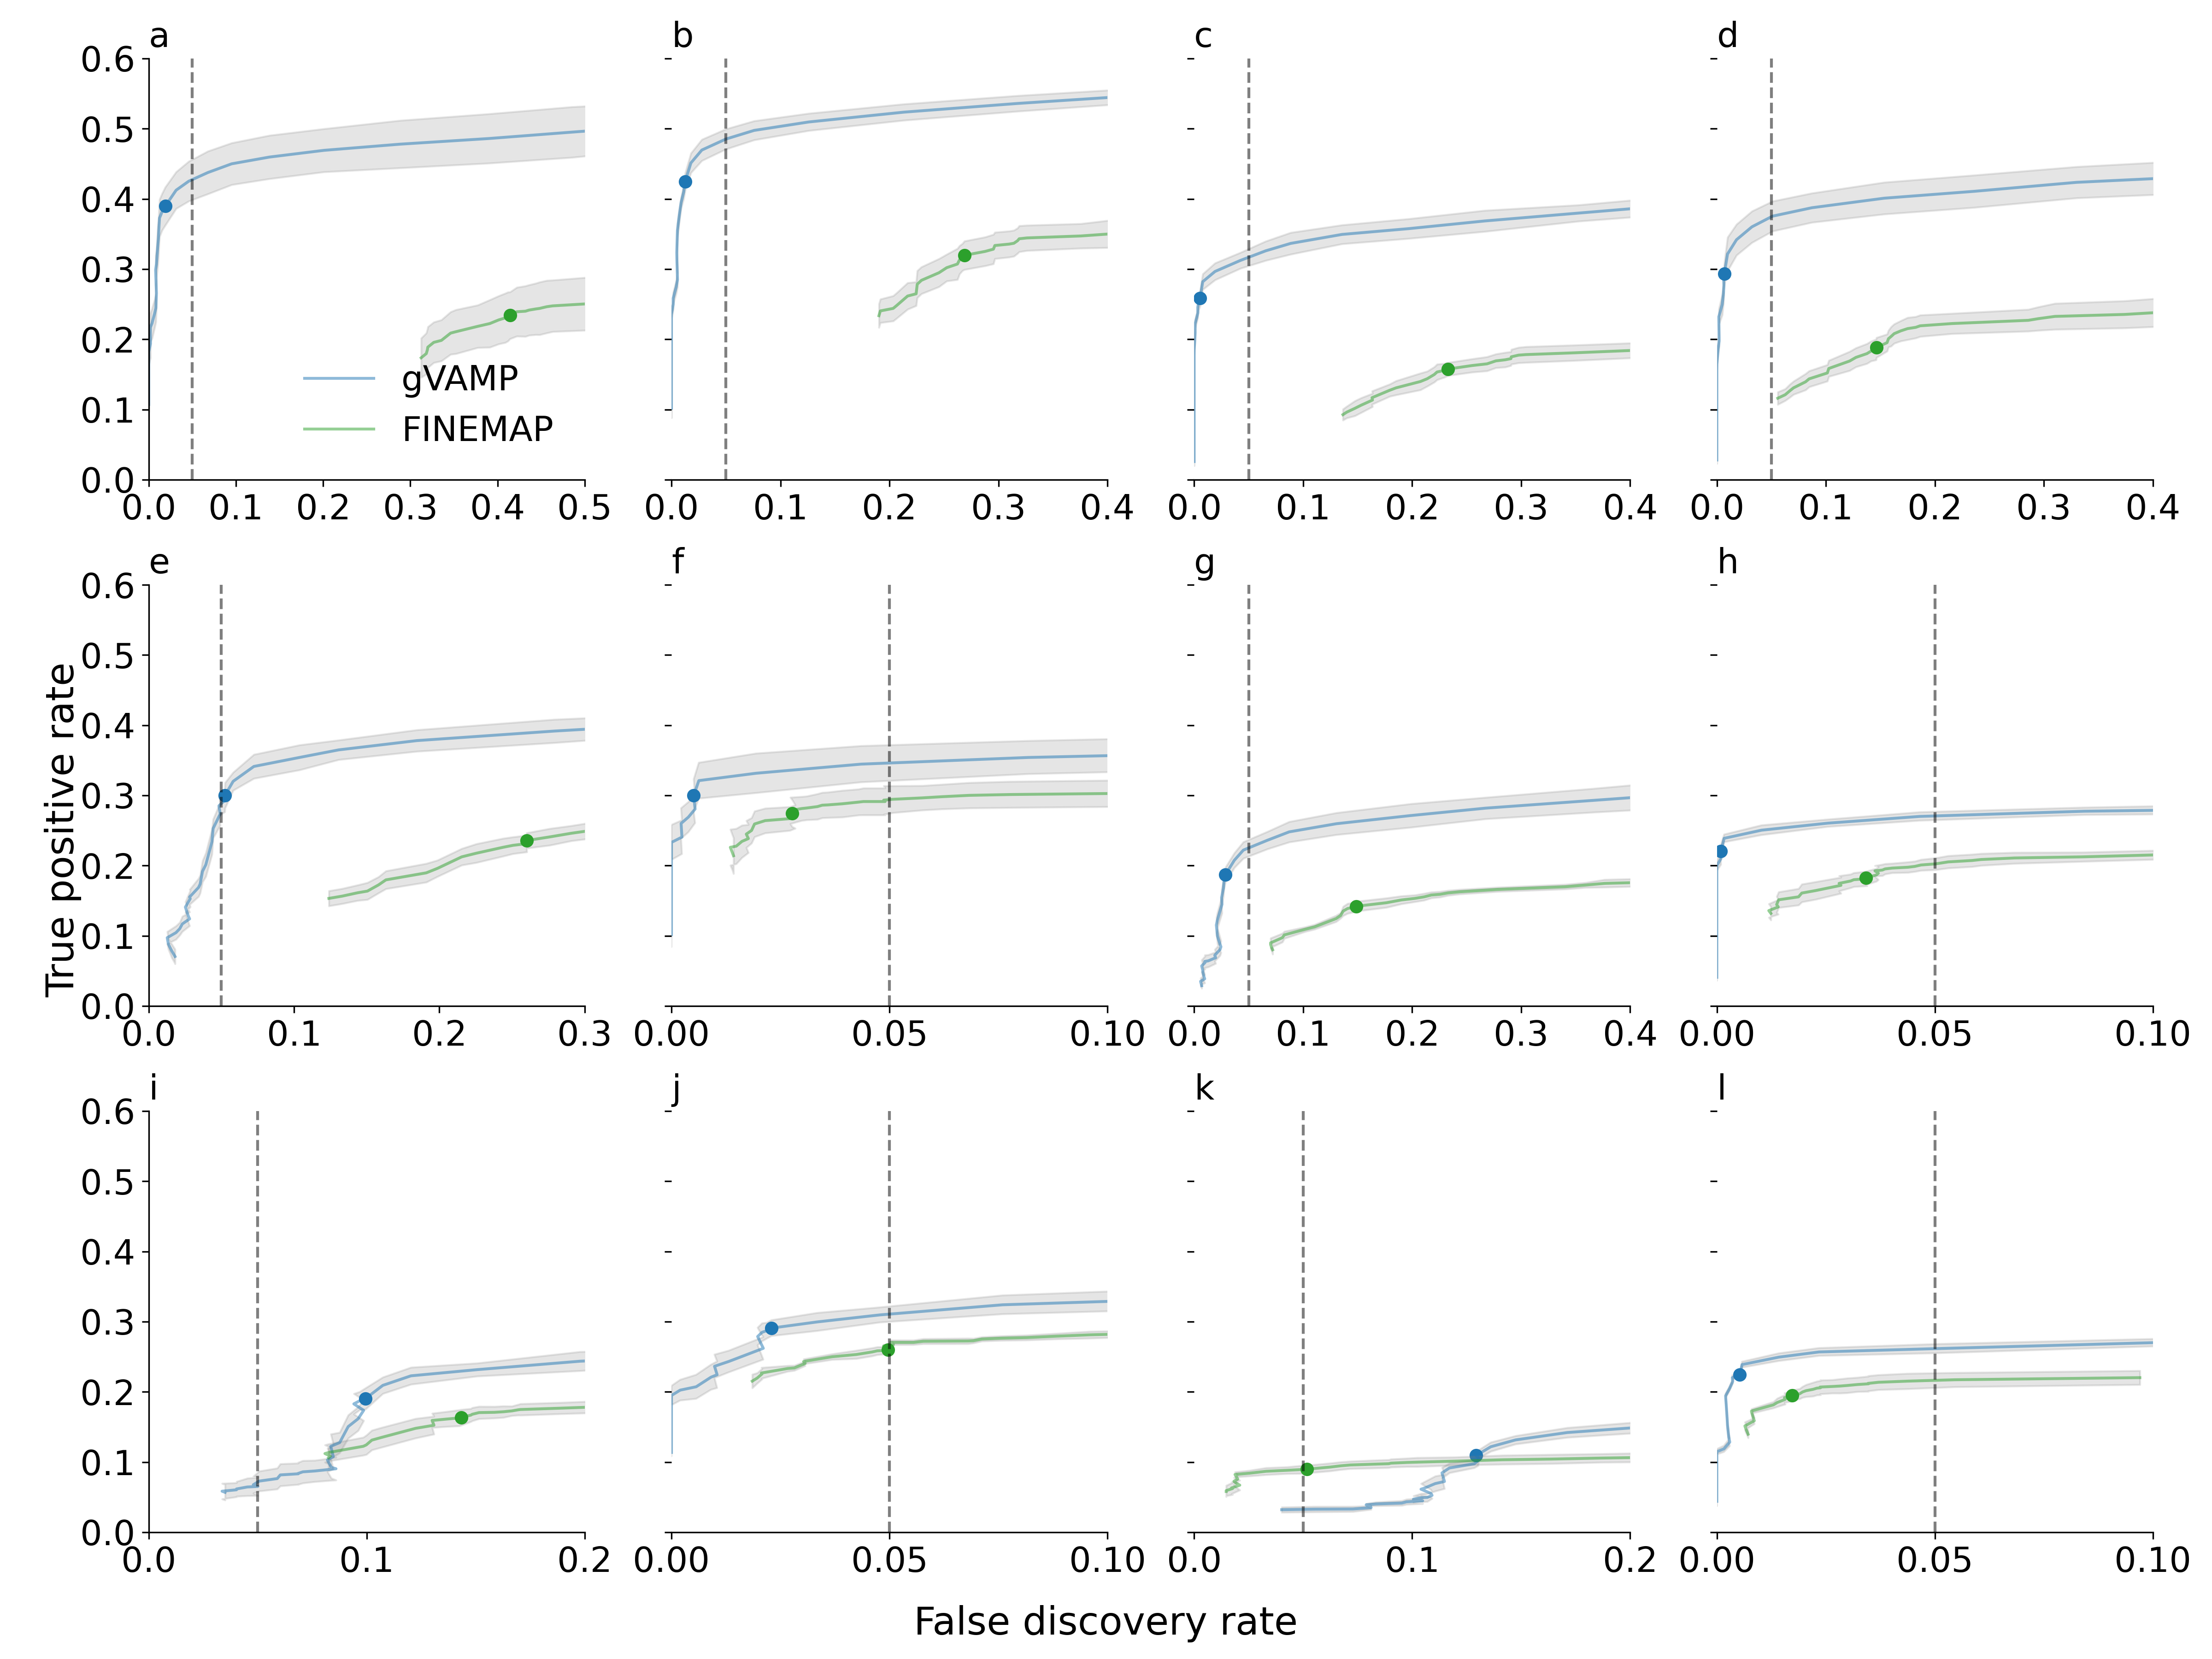
\includegraphics[width=\linewidth]{graphics/gVAMP_figures/v4/FigS1.png}
    \caption[Comparison of the true positive rate (TPR, $y$-axis) versus the false discovery rate (FDR, $x$-axis) between gVAMP and marginal GWAS association testing plus fine-mapping implemented in the FINEMAP algorithm across 12 simulation scenarios using whole genome sequence (WGS) data of chromosomes 11 to 15 in the UK Biobank]{\textbf{Comparison of the true positive rate (TPR, $y$-axis) versus the false discovery rate (FDR, $x$-axis) between gVAMP and marginal GWAS association testing plus fine-mapping implemented in the FINEMAP algorithm across 12 simulation scenarios using whole genome sequence (WGS) data of chromosomes 11 to 15 in the UK Biobank.} \small For the detailed description of different simulation settings, see Methods and Supplementary Table \ref{table:S1}. We use a Bonferroni corrected p-value significance threshold for marginal GWAS testing and then having identified associated regions we examine the ability of FINEMAP (green) to conduct variable selection across posterior inclusion probability (PIP) thresholds. For gVAMP (blue), variable selection is conducted from PIP values obtained from a single model run genome-wide. Error bands give the standard deviation across 5 simulation replicates. The blue and green dots give the TPR and FDR at PIP $\geq 0.95$, which should correspond to an FDR of $\leq 0.05$ if the model correctly conducts variable selection based on PIP values.}
    \label{fig:finalFigS1}
\end{figure}

\newpage

\begin{figure}[!htp]
    \centering
    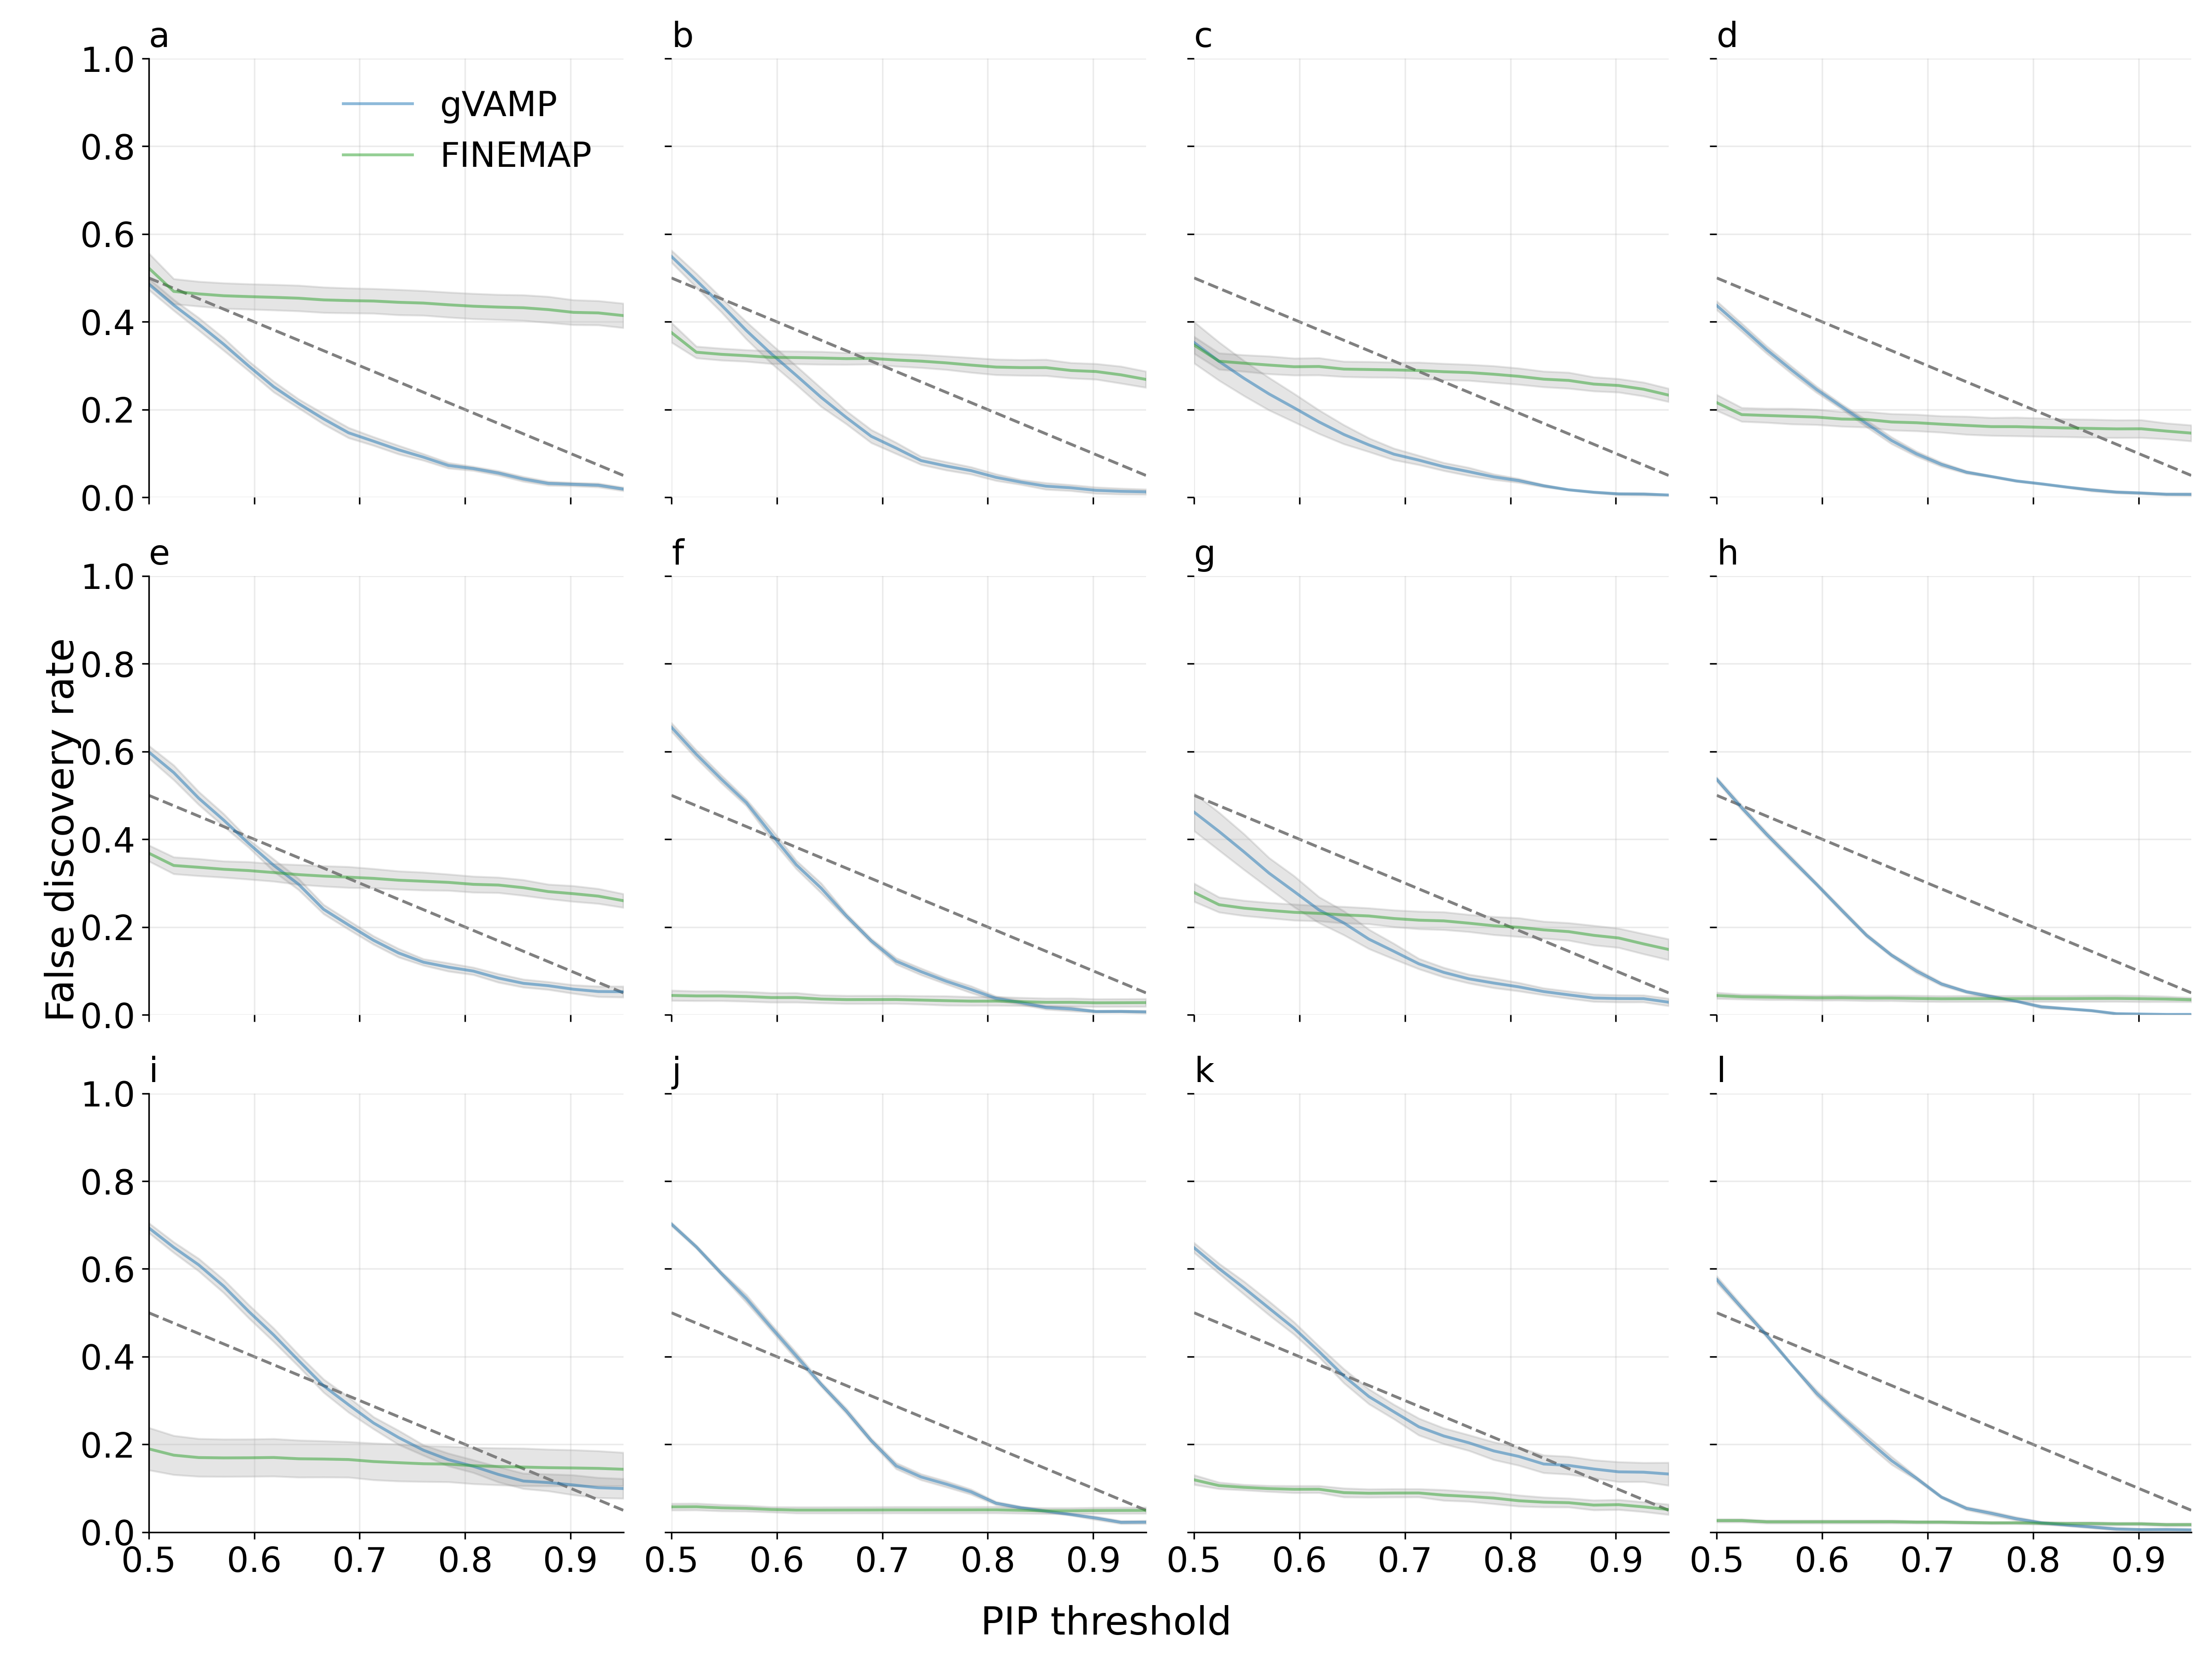
\includegraphics[width=\linewidth]{graphics/gVAMP_figures/v4/FigS2.png}
    \caption[Comparison of the posterior inclusion probability threshold (PIP threshold, $x$-axis) versus the false discovery rate (FDR, $y$-axis) between gVAMP and marginal GWAS association testing plus fine-mapping implemented in the FINEMAP algorithm across 12 simulation scenarios using whole genome sequence data of chromosomes 11 to 15 in the UK Biobank]{\textbf{Comparison of the posterior inclusion probability threshold (PIP threshold, $x$-axis) versus the false discovery rate (FDR, $y$-axis) between gVAMP and marginal GWAS association testing plus fine-mapping implemented in the FINEMAP algorithm across 12 simulation scenarios using whole genome sequence (WGS) data of chromosomes 11 to 15 in the UK Biobank.} \small For the detailed description of different simulation settings, see Methods and Supplementary Table \ref{table:S1}. We use a Bonferroni corrected p-value significance threshold for marginal GWAS testing and then having identified associated regions we examine the ability of FINEMAP (green) to conduct variable selection across PIP thresholds. For gVAMP (blue), variable selection is conducted from PIP values obtained from a single model run genome-wide. Error bands give the standard deviation across 5 simulation replicates. Dashed lines gives the maximum FDR expected at different PIP thresholds for a model that correctly conducts variable selection based on PIP values.}
    \label{fig:finalFigS2}
\end{figure}

\newpage

\begin{figure}[!htp]
    \centering
    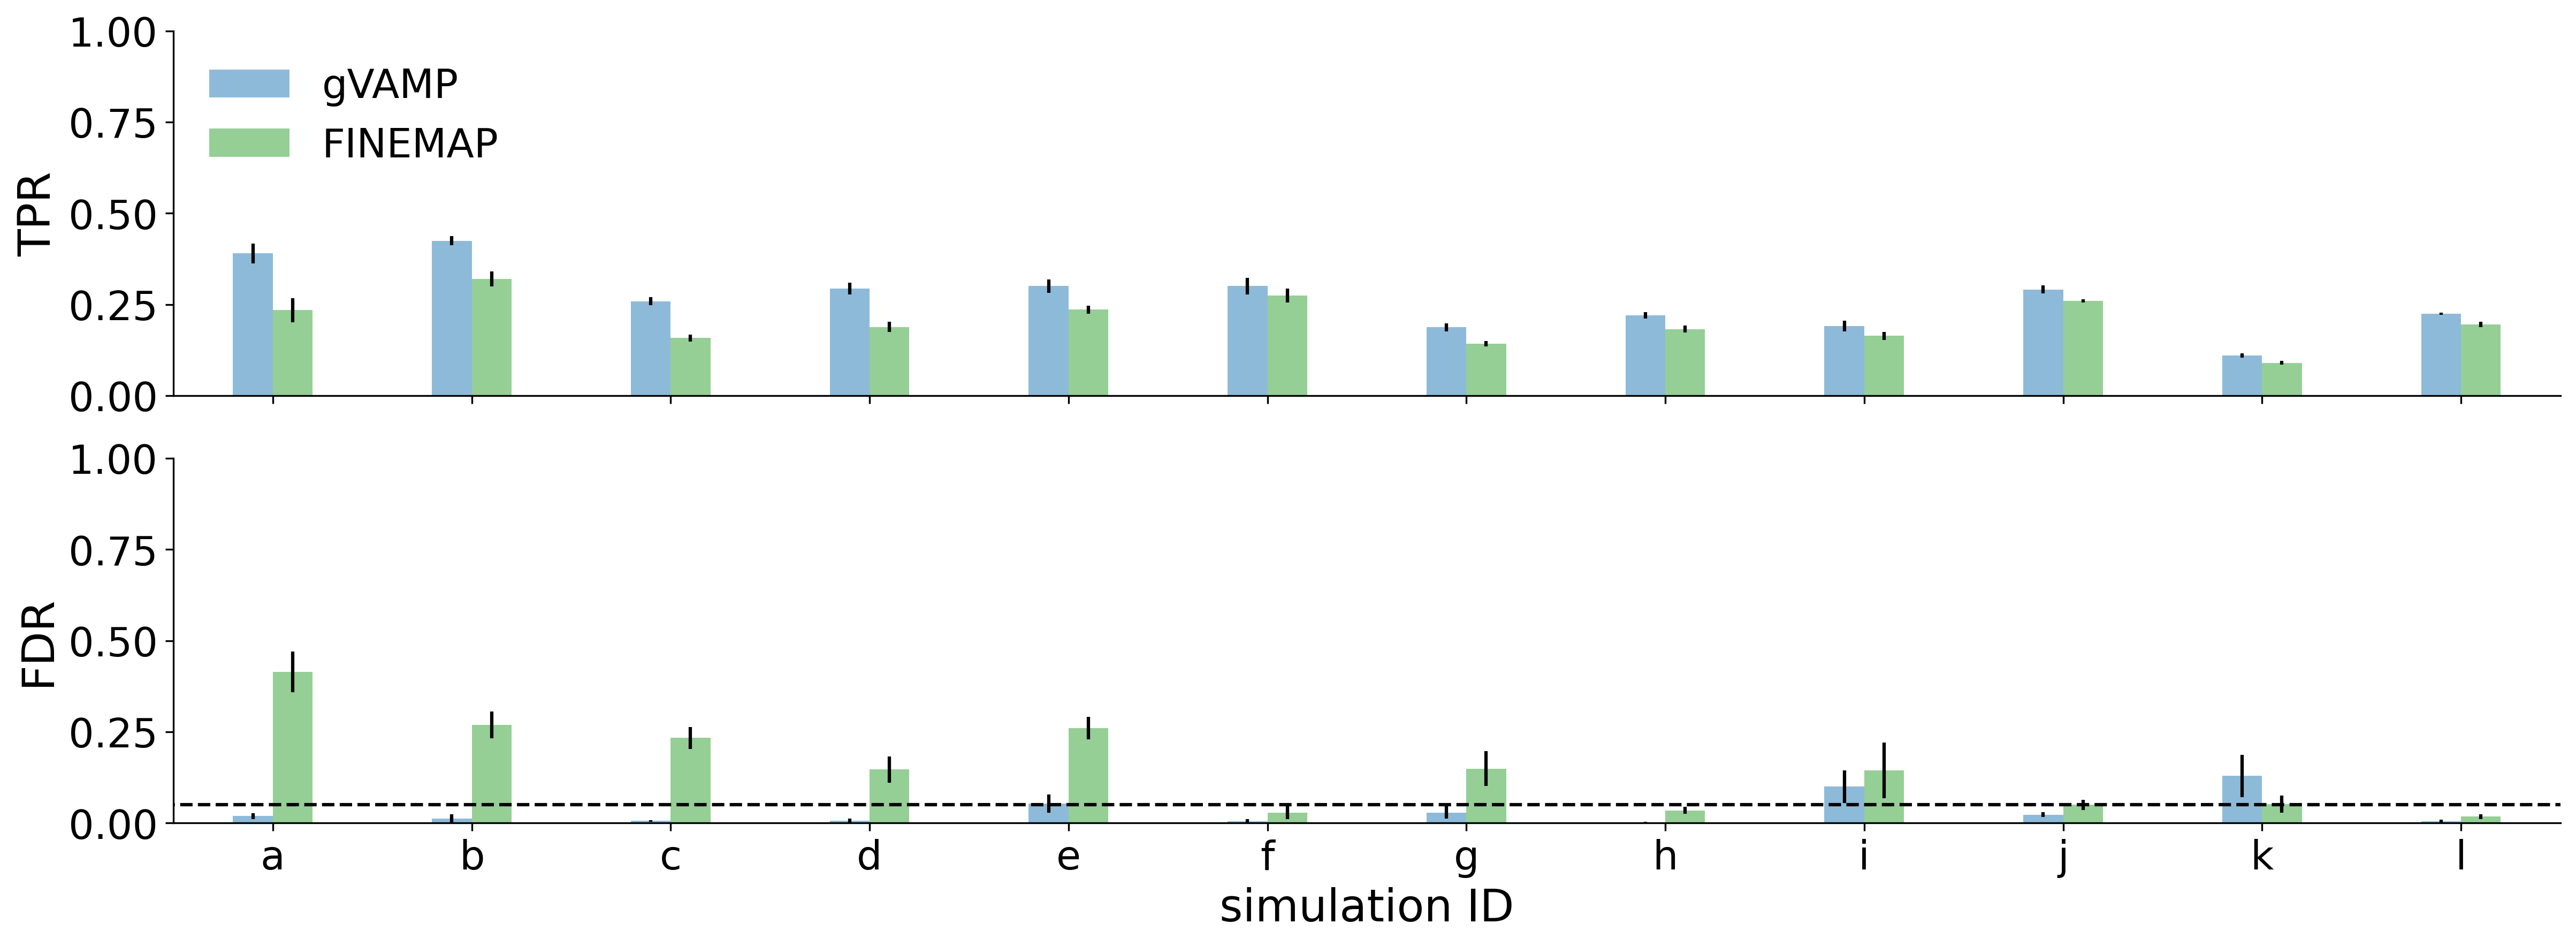
\includegraphics[width=\linewidth]{graphics/gVAMP_figures/v4/FigS3.png}
    \caption[Performance in terms of the true positive rate (TPR) and the false discovery rate (FDR) of marginal GWAS testing plus fine-mapping with FINEMAP, and gVAMP at posterior inclusion probability $\ge 0.95$ in a whole genome sequence data simulation study of chromosomes 11 to 15 in the UK Biobank]{\textbf{Performance in terms of the true positive rate (TPR) and the false discovery rate (FDR) of marginal GWAS testing plus fine-mapping with FINEMAP, and gVAMP at posterior inclusion probability $\ge 0.95$ in a whole genome sequence (WGS) data simulation study of chromosomes 11 to 15 in the UK Biobank.} \small We use a Bonferroni corrected p-value significance threshold for marginal GWAS and PIP $>0.95$ for FINEMAP (green) applied for regions identified as significant in the marginal analysis. FINEMAP controls the FDR in only 5 out of 12 WGS data simulation settings (see Methods and Supplementary Table \ref{table:S1}). In contrast, using a PIP $>0.95$ threshold for the gVAMP testing (blue) controls FDR in 10 out of 12 settings, whilst yielding consistently higher TPR across all settings. Error bars give the standard deviation across 5 simulation replicates.}
    \label{fig:finalFigS3}
\end{figure}

\newpage

\begin{figure}[!htp]
    \centering
    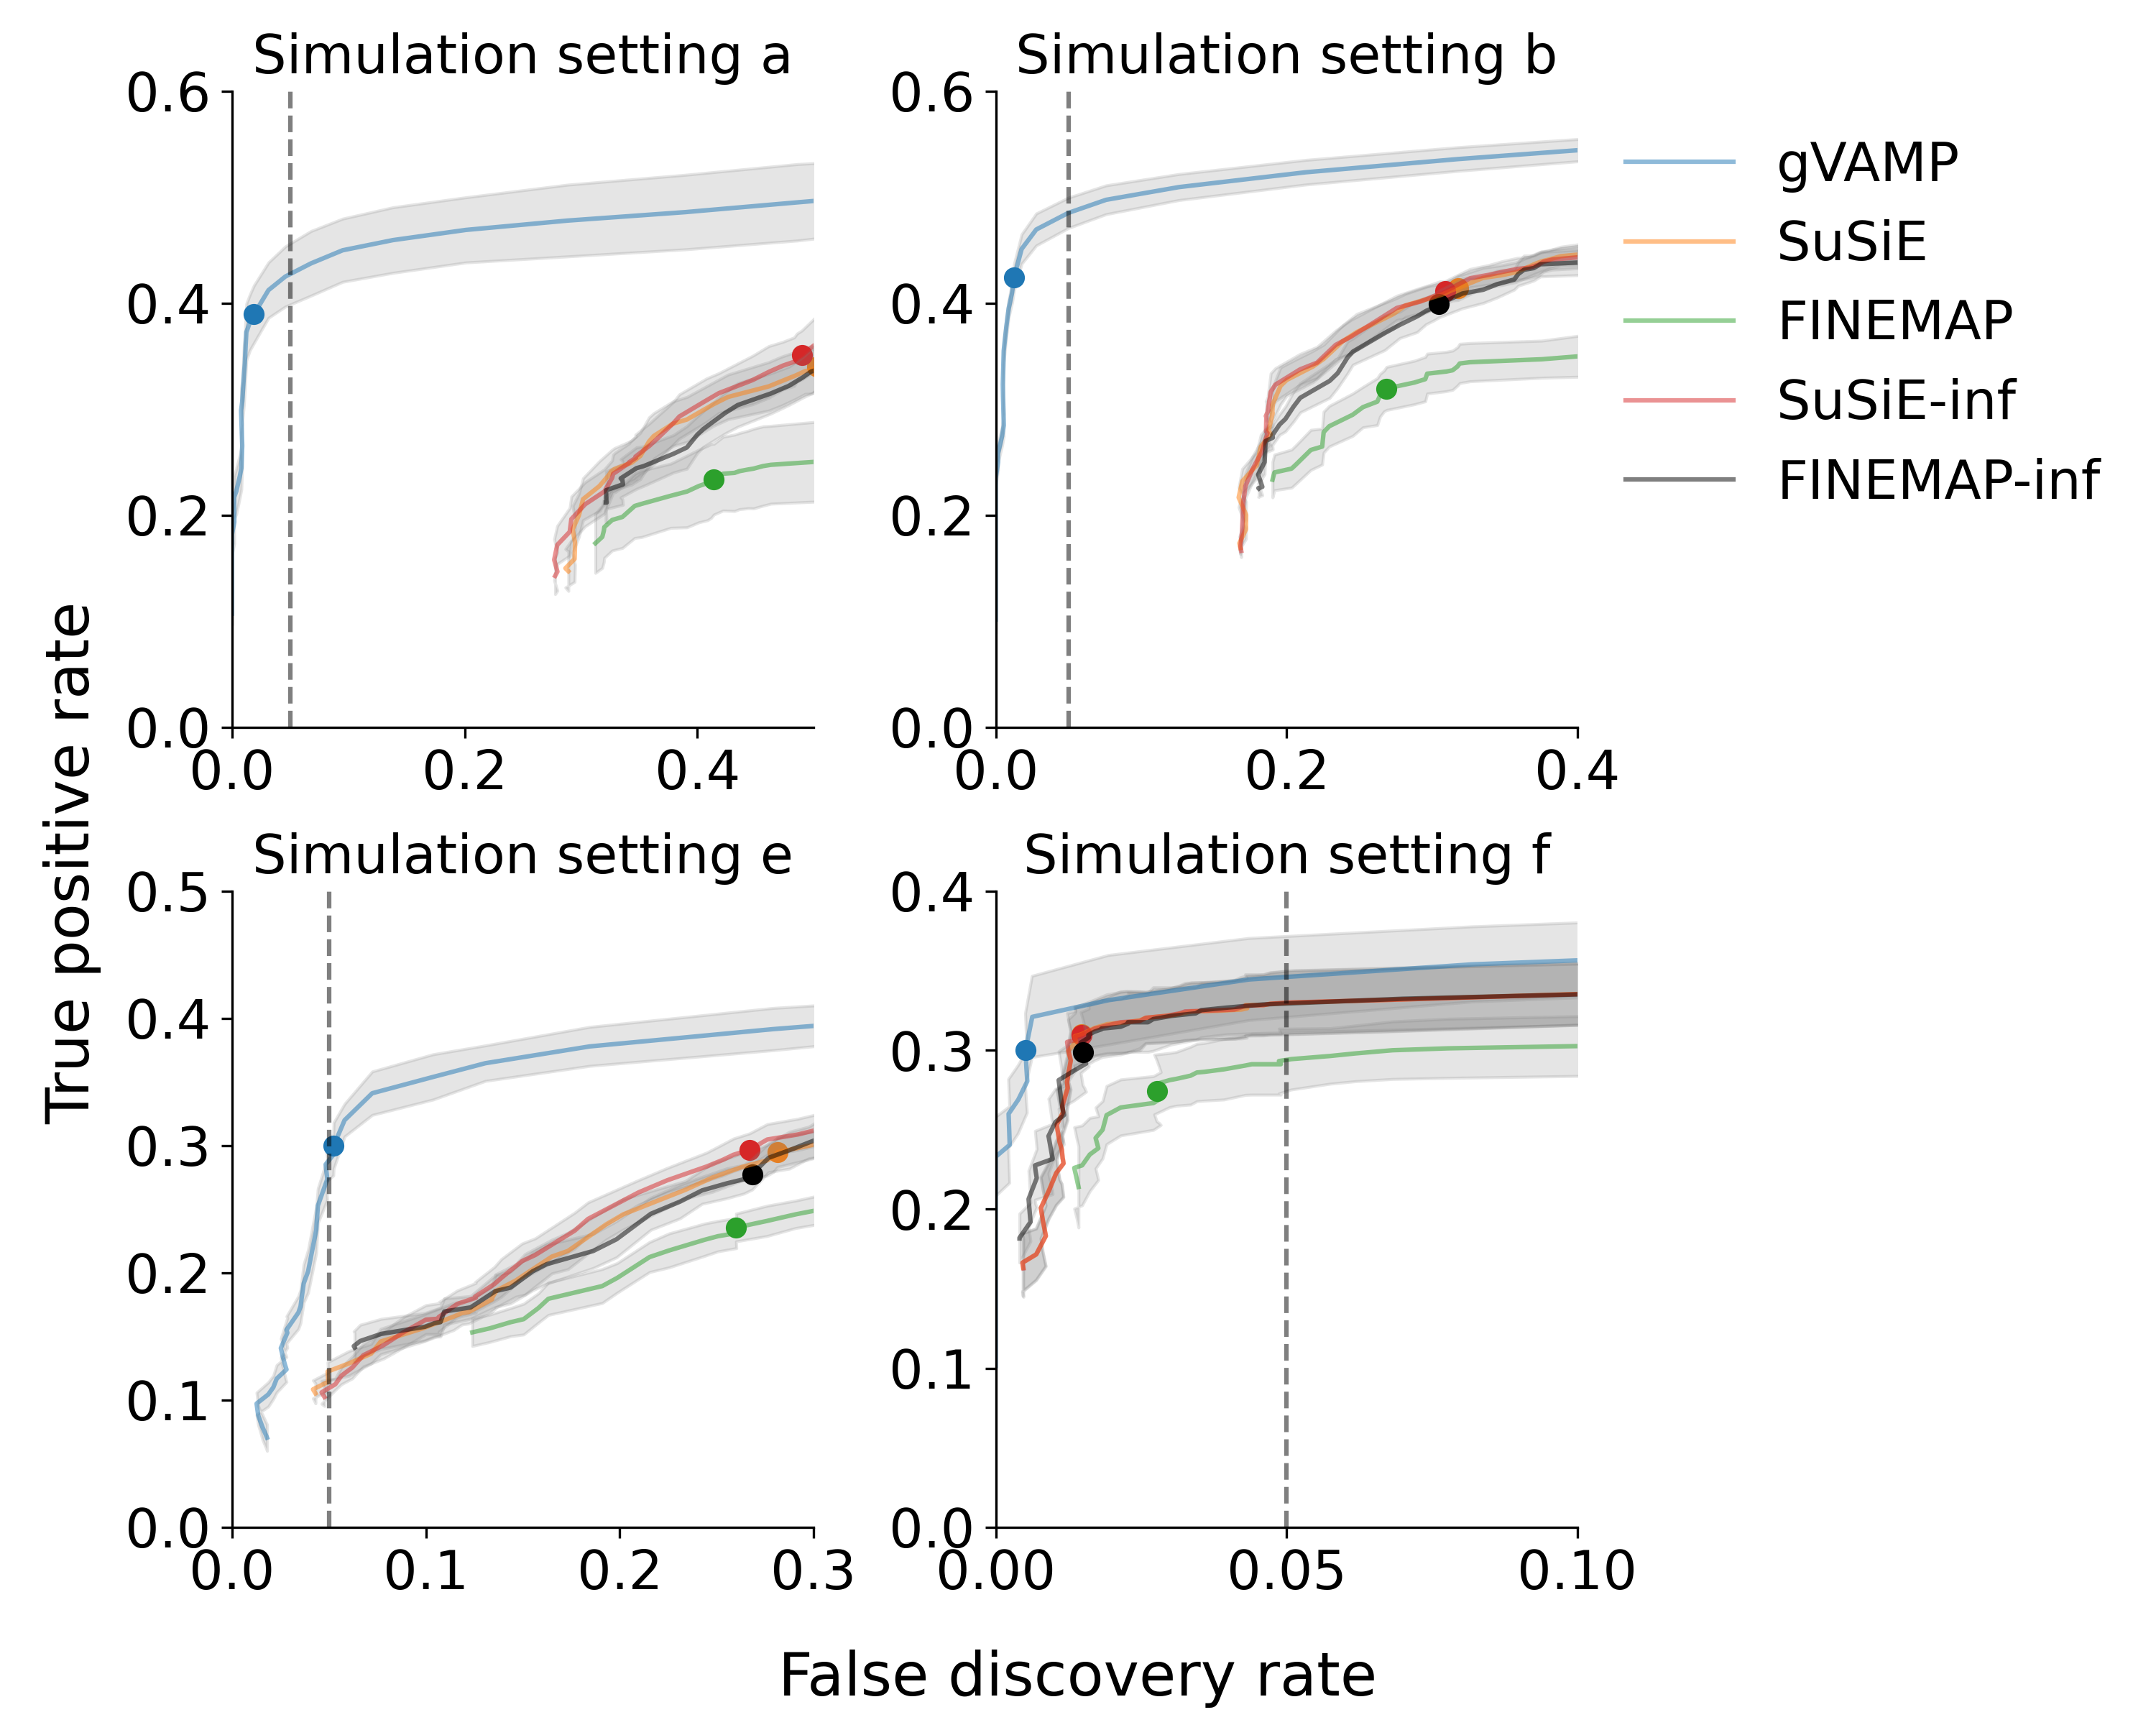
\includegraphics[width=\linewidth]{graphics/gVAMP_figures/v4/FigS4.png}
    \caption[Benchmarking of gVAMP to a wide range of fine-mapping methods applied to marginal GWAS summary data in a whole genome sequence data simulation study of chromosomes 11 to 15 in the UK Biobank]{\textbf{Benchmarking of gVAMP to a wide range of fine-mapping methods applied to marginal GWAS summary data in a whole genome sequence (WGS) data simulation study of chromosomes 11 to 15 in the UK Biobank.} \small For the detailed description of different simulation settings, see Methods and Supplementary Table \ref{table:S1}. We use a Bonferroni corrected p-value significance threshold for marginal GWAS testing and then having identified associated regions we apply FINEMAP (green) and SuSiE (orange) to conduct variable selection across PIP thresholds. We also compare to SuSiE-inf (red) and FINEMAP-inf (black) run genome-wide. We compare the true positive rate (TPR) and false discovery rate (FDR) of the methods, with coloured dots indicating the TPR and FDR at $\geq 0.95$ PIP, lines giving the TPR and FDR across PIP thresholds and error bands giving the standard deviation across 5 simulation replicates. SuSiE-inf and FINEMAP-inf improve the TPR, but generally not the FDR. gVAMP gives consistently higher TPR at FDR $\leq 5\%$.}
    \label{fig:finalFigS7}
\end{figure}

\newpage

\begin{figure}[!htp]
    \centering
    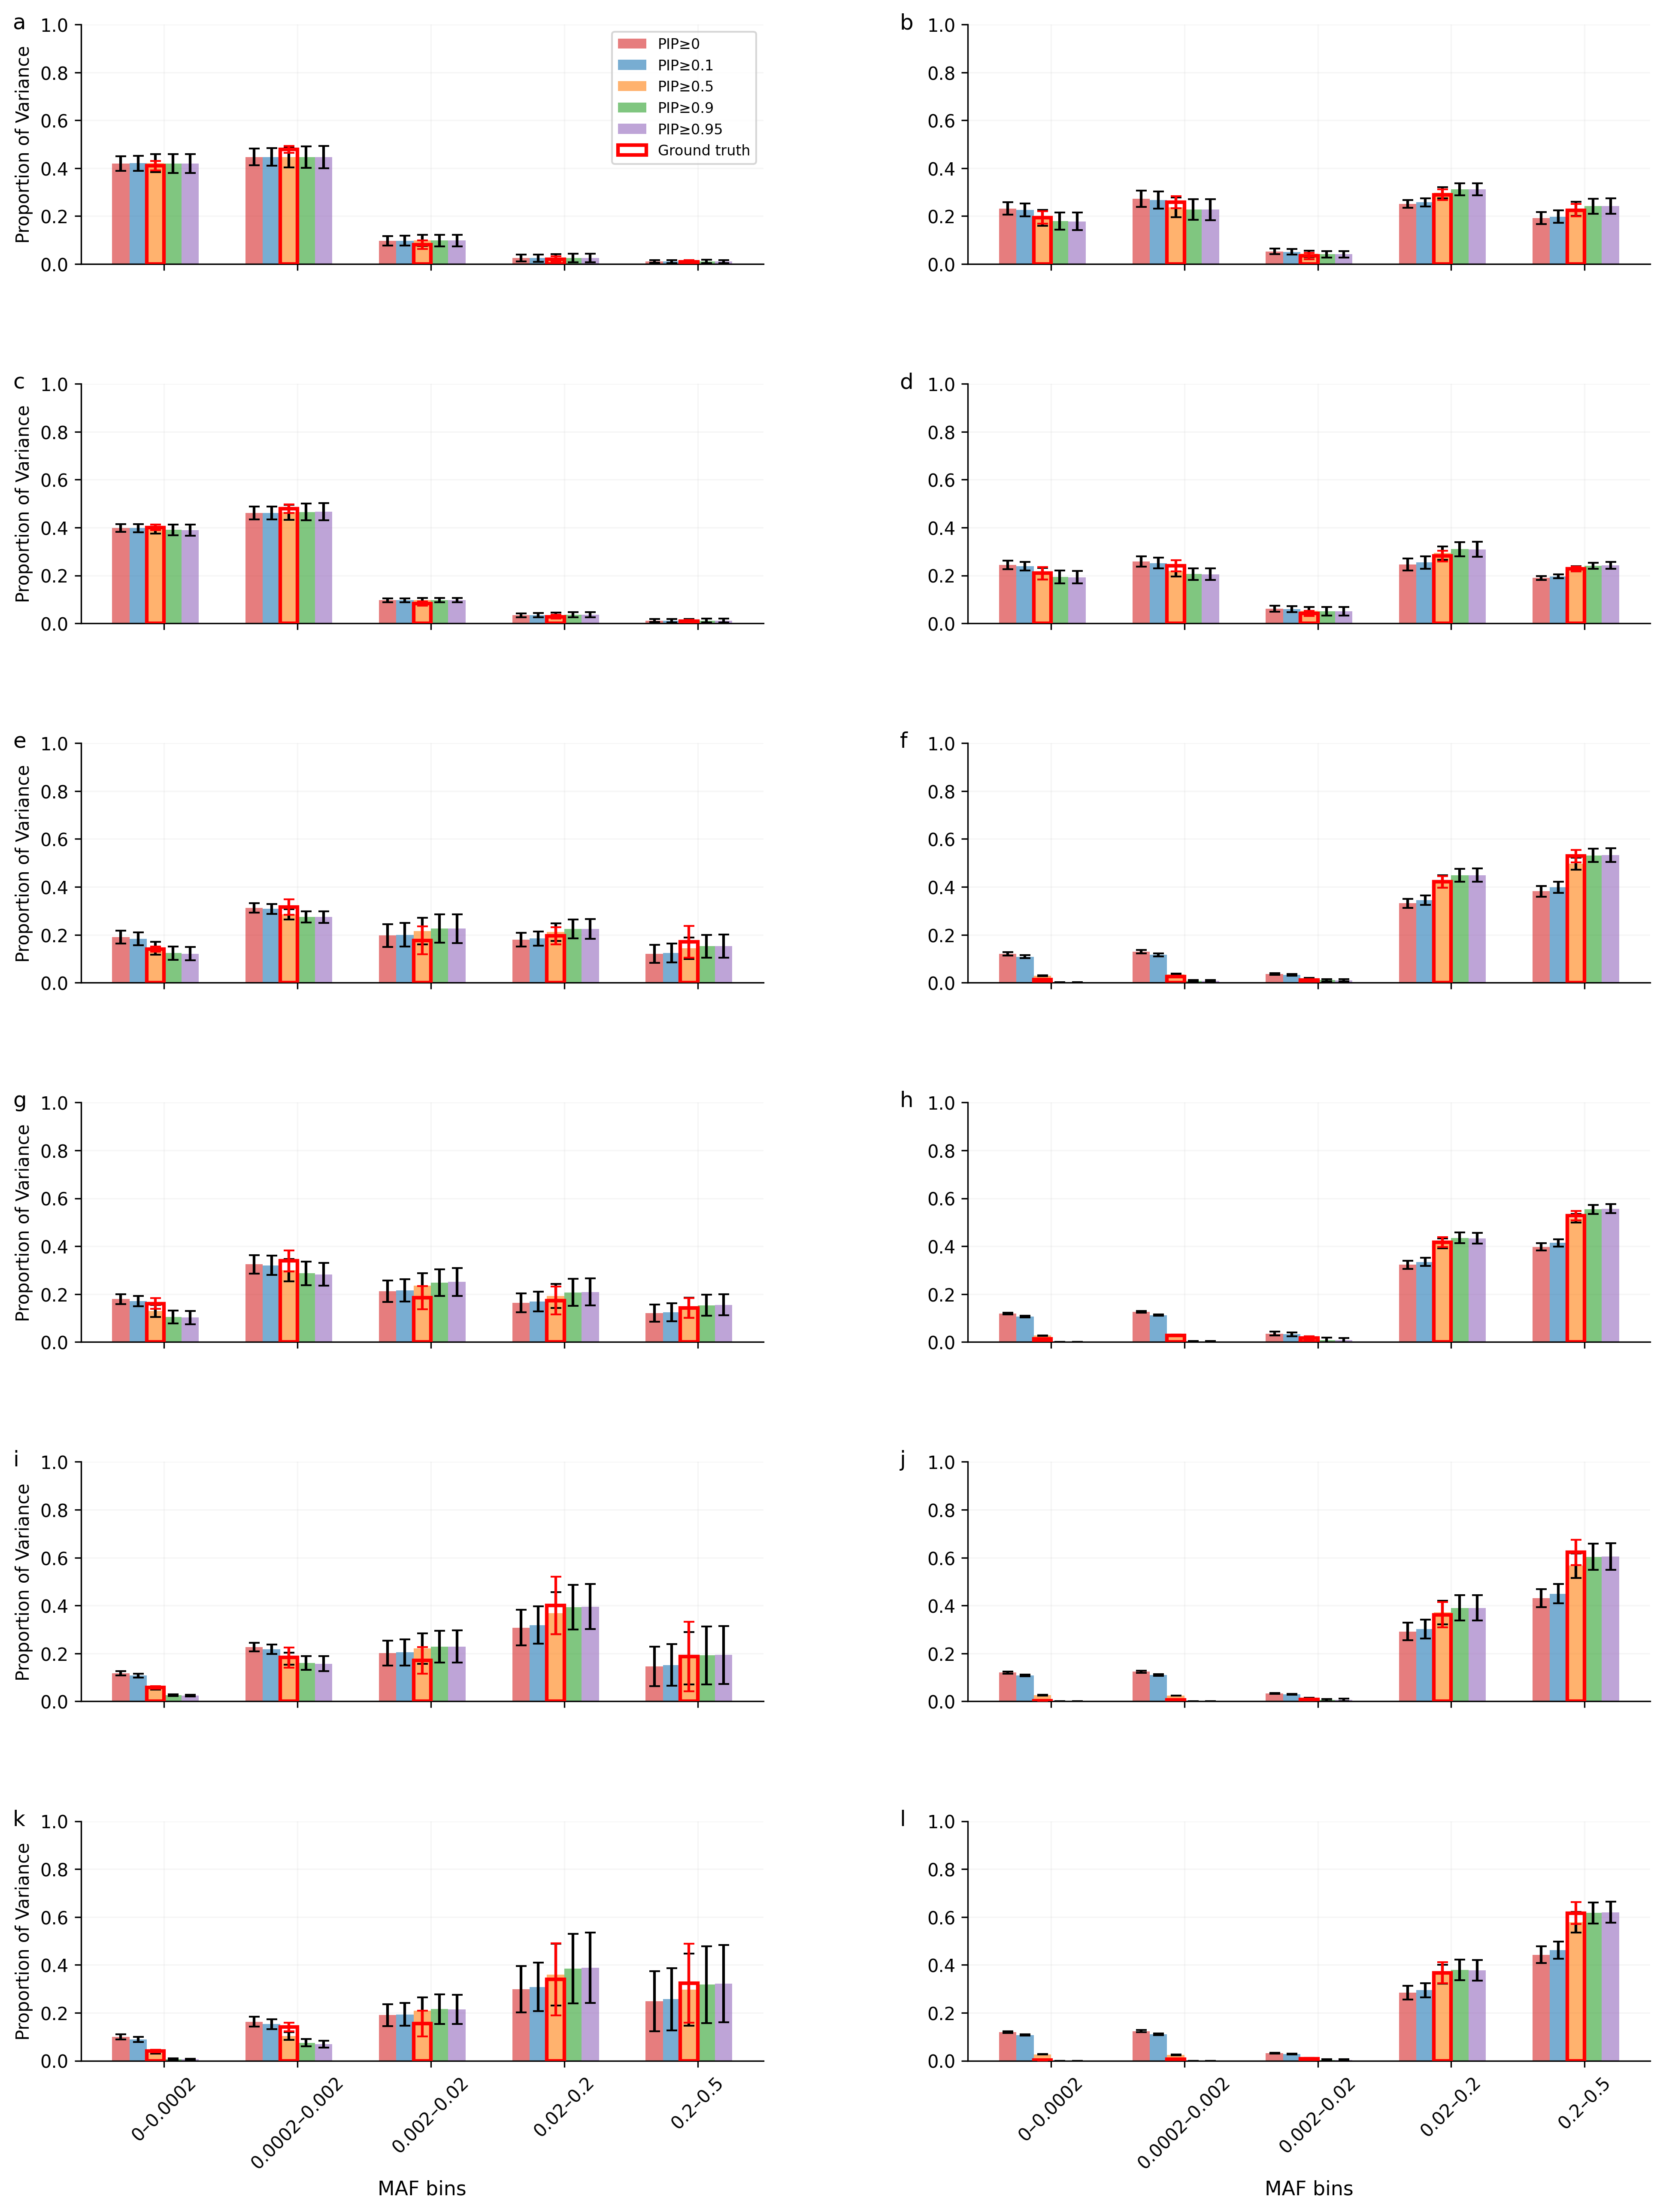
\includegraphics[width=0.9\linewidth]{graphics/gVAMP_figures/v4/FigS5.png}
    \caption[The proportion of variance attributable to DNA loci of different frequency in a whole genome sequence data simulation study using chromosomes 11 to 15 of the UK Biobank]{\textbf{The proportion of variance attributable to DNA loci of different frequency in a whole genome sequence (WGS) data simulation study using chromosomes 11 to 15 of the UK Biobank}. \small We plot the proportion of the sum of the squared regression coefficients attributable to variants of different frequency as estimated from gVAMP across different posterior inclusion probability (PIP) thresholds. The ground truth (red frame) is calculated as the sum of squared true effects across different frequency groups. The variance attributable to SNPs of different frequency matches the ground truth when selecting variants at posterior inclusion probability $\geq 0.5$. Error bars give the standard deviation across 5 simulation replicates.}
    \label{fig:finalFigS4}
\end{figure}

\newpage

\begin{figure}[!htp]
    \centering
    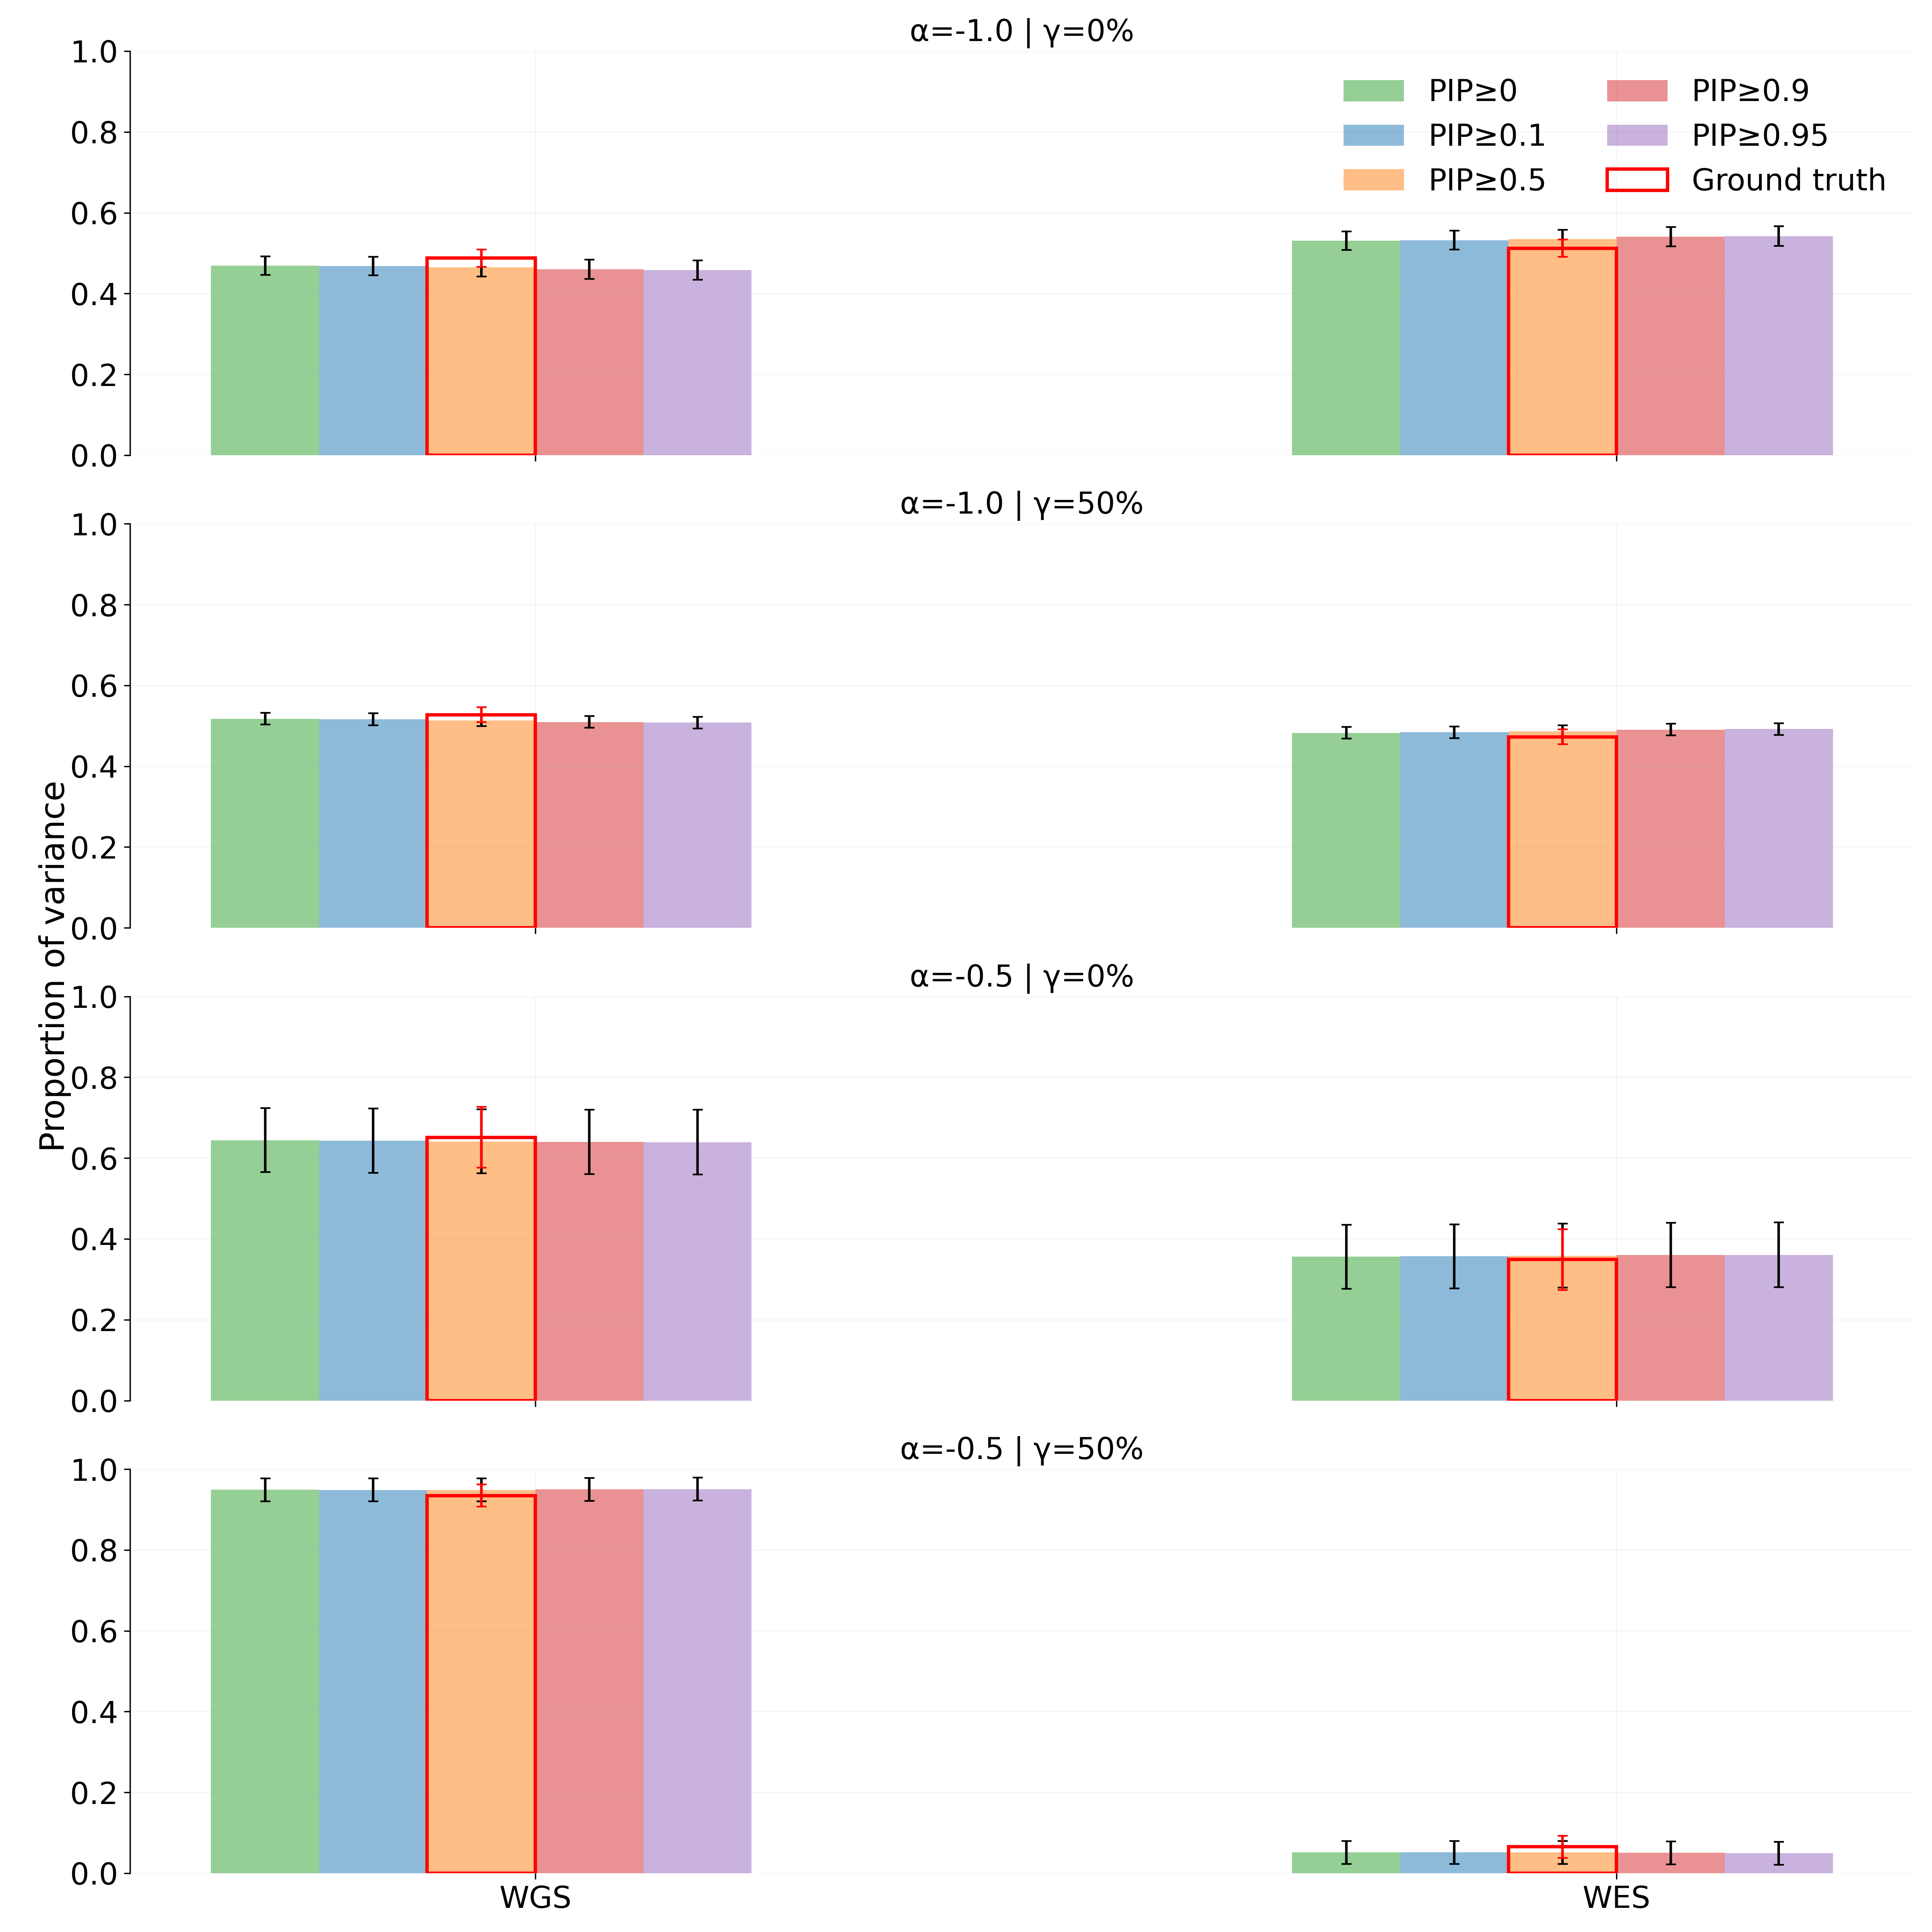
\includegraphics[width=\linewidth]{graphics/gVAMP_figures/v4/FigS6.png}
    \caption[Simulation study including whole exome sequence (WES) burden scores alongside WGS variants from chromosomes 11 to 15 of the UK Biobank]{\textbf{Simulation study including WES burden scores alongside WGS variants from chromosomes 11 to 15 of the UK Biobank}. We simulate 500 underlying causal signals with a total heritability of $h^2=7.25\%$, allocating 75\% of signals to WGS variants and 25\% to WES burden scores, with WES burden scores exhibiting effect sizes three-fold larger than those of individual WGS variants. For the detailed description of $\alpha$ and $\gamma$ parameters, see Methods. We find that the variance explained by WES and WGS, as inferred by gVAMP, aligns well with the ground truth across a range of PIP thresholds.}
    \label{fig:S6}
\end{figure}

\newpage

\begin{figure}[H]
    \centering
    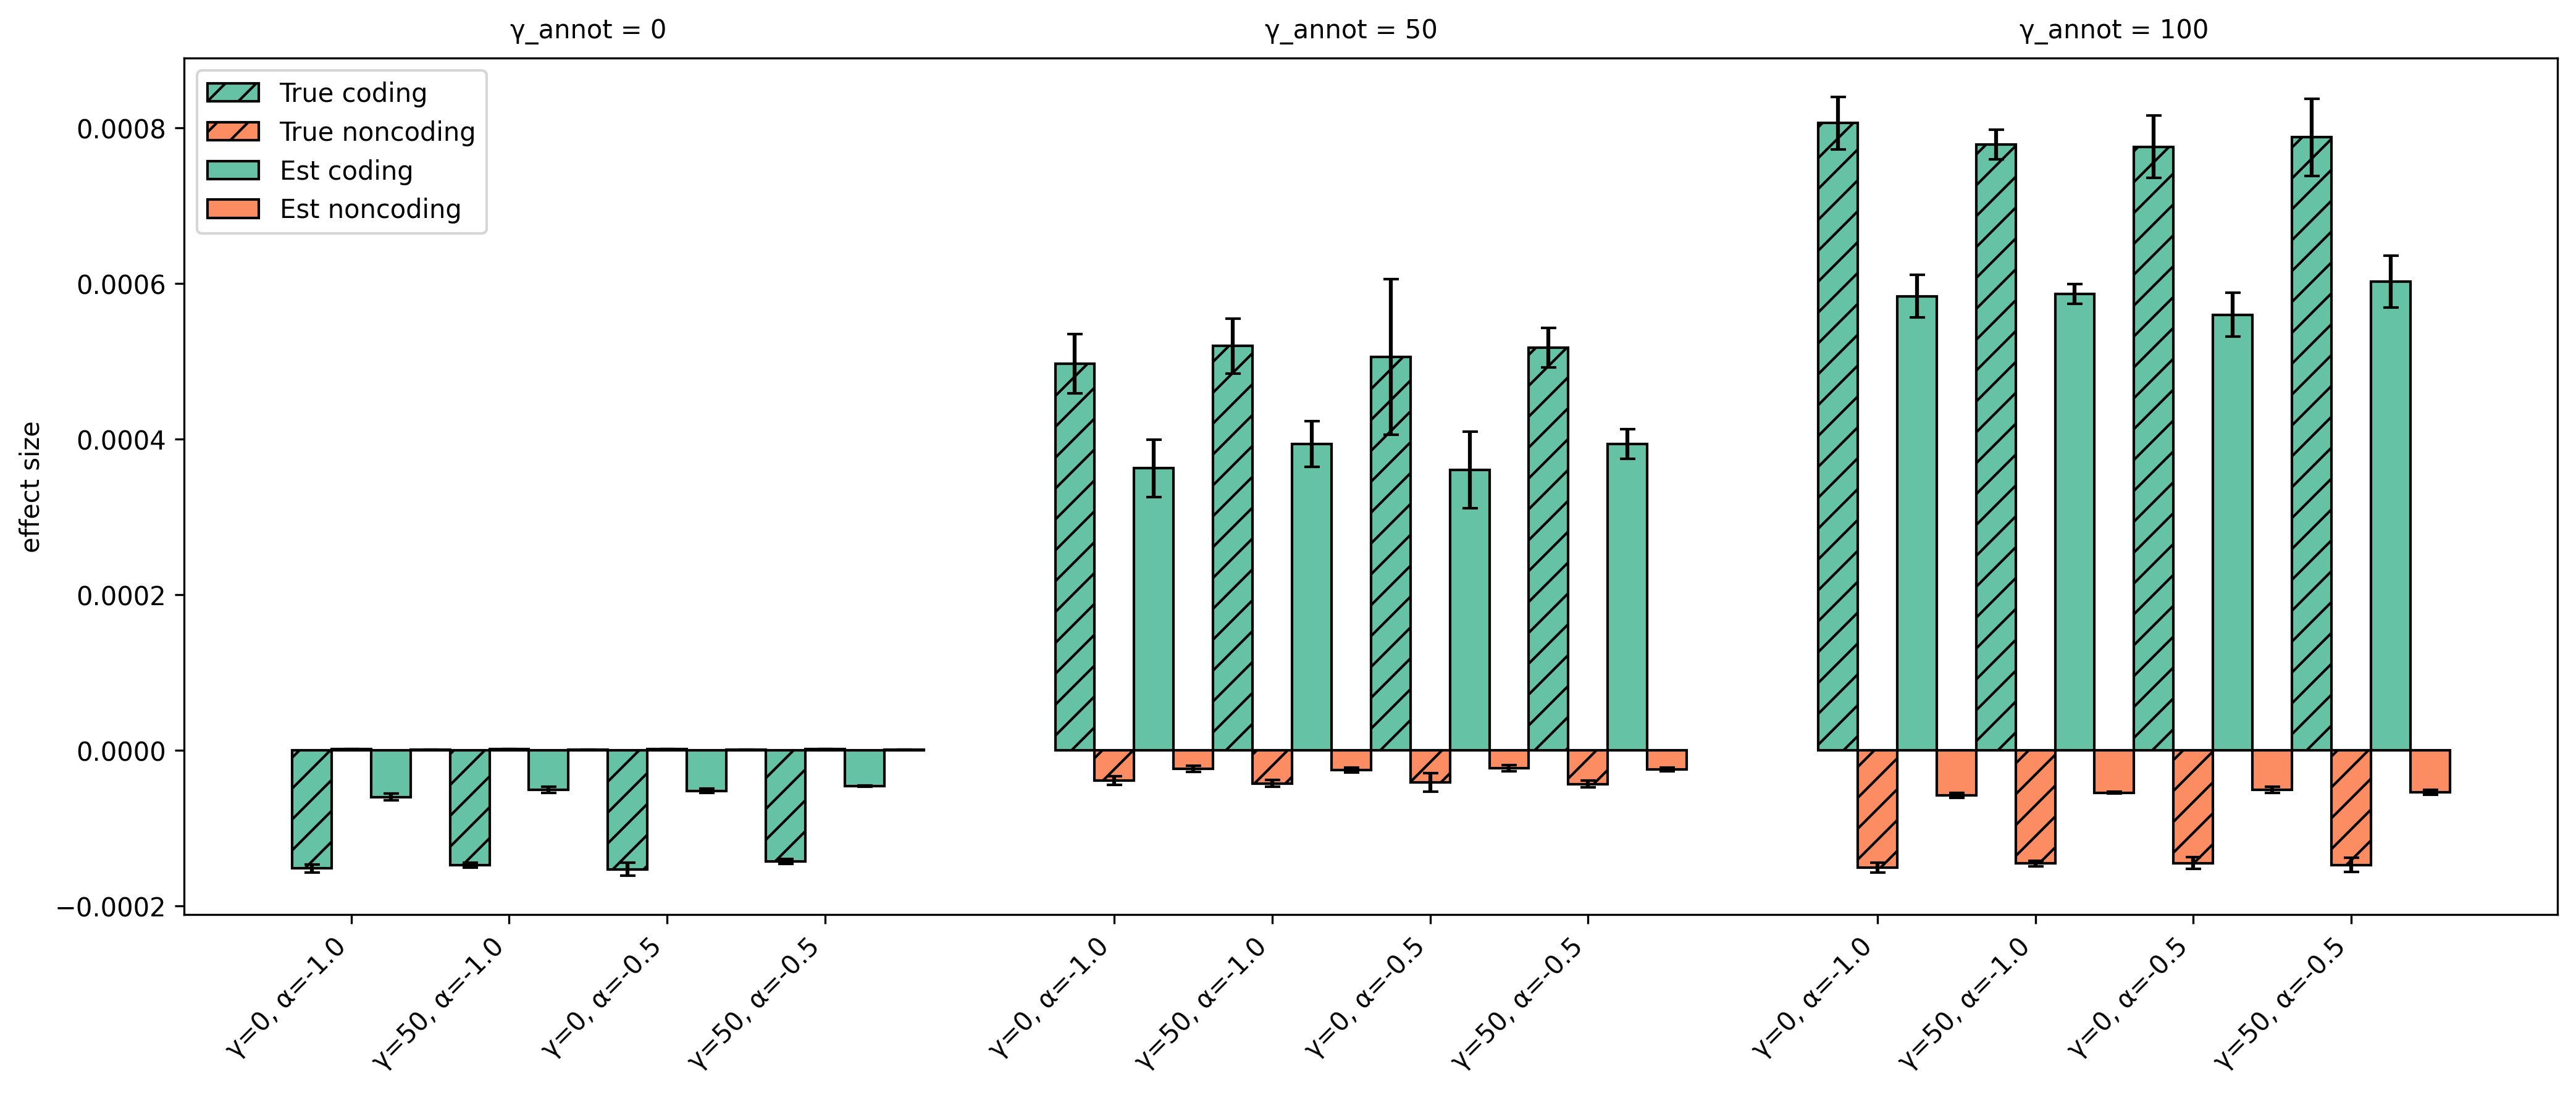
\includegraphics[width=\linewidth]{graphics/gVAMP_figures/cellgen_review/effect_size_plot_threshold_0.0.png}
    \caption[Simulation study stratifying causal effects into coding and non-coding regions]{\textbf{Simulation study stratifying causal effects into coding and non-coding regions.} We simulate 500 signals with a total heritability of $h^2=7.25\%$ across a variety of settings for power law $\alpha$ and percentage of common variants $\gamma$, also allocating $\gamma_\text{annot} \in \{0, 50, 100 \}$ \% percentage of causal variants to the coding region of the DNA. Effect sizes ($y$-axis) are calculated as the difference of the group average absolute value of the effects from the total group average absolute value of the effect (enrichment). The true simulated values are given by boxes with diagonal lines.}
    \label{fig:S7new}
\end{figure}

\newpage

\begin{figure}[!htp]
    \centering
    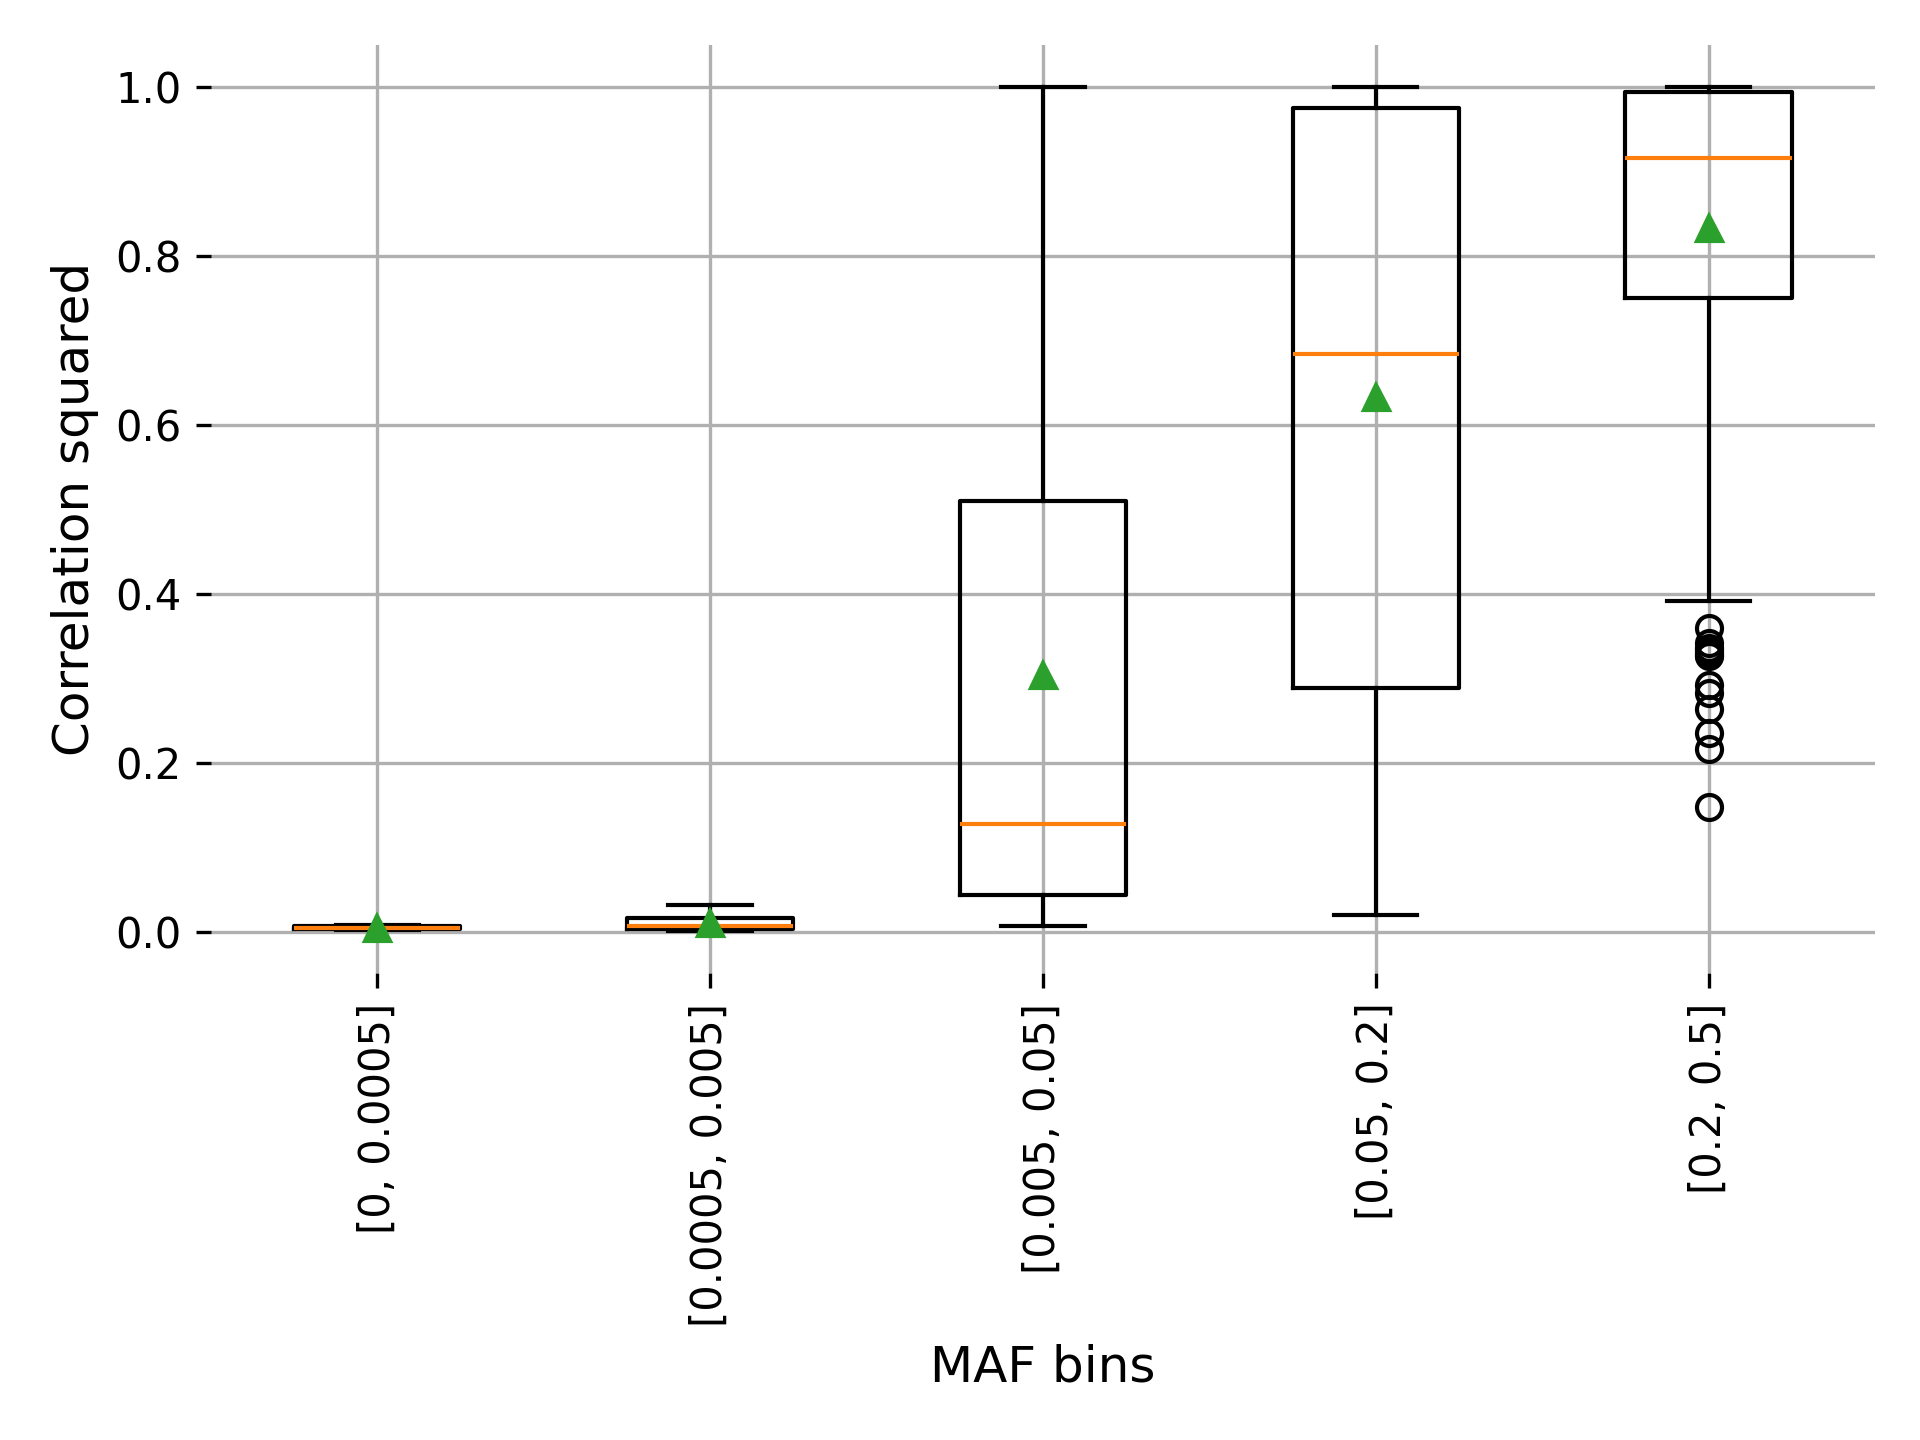
\includegraphics[width=\linewidth]{graphics/gVAMP_figures/v4/FigS8.png}
    \caption[Distribution of the maximum squared correlation between each height-associated variant found by gVAMP and variants reported by Yengo \textit{et al.} \cite{HTbig} within a 1Mb window across MAF groups]{\textbf{Distribution of the maximum squared correlation between each height-associated variant found by gVAMP and variants reported by Yengo \textit{et al.} \cite{HTbig} within a 1Mb window across MAF groups.} We estimate the maximum correlation within the UK Biobank WGS data of each gVAMP discovery at PIP$\geq95\%$ with Yengo \emph{et al.} SNPs significant at $p\le5 \cdot 10^{-8}$ within a 1 Mb window and stratify the squared correlations by the MAF of the gVAMP discovered variant. The orange line depicts the median, while the green triangle indicates the mean value. In total, we find 432 SNPs with correlation squared greater than 0.1. The results suggest that very rare variants (MAF $\le 0.005$) are independent of the colocalizing common variants from \cite{HTbig}.}
    \label{fig:correlation_MAF}
\end{figure}

\newpage

\begin{figure}[!htp]
    \centering
    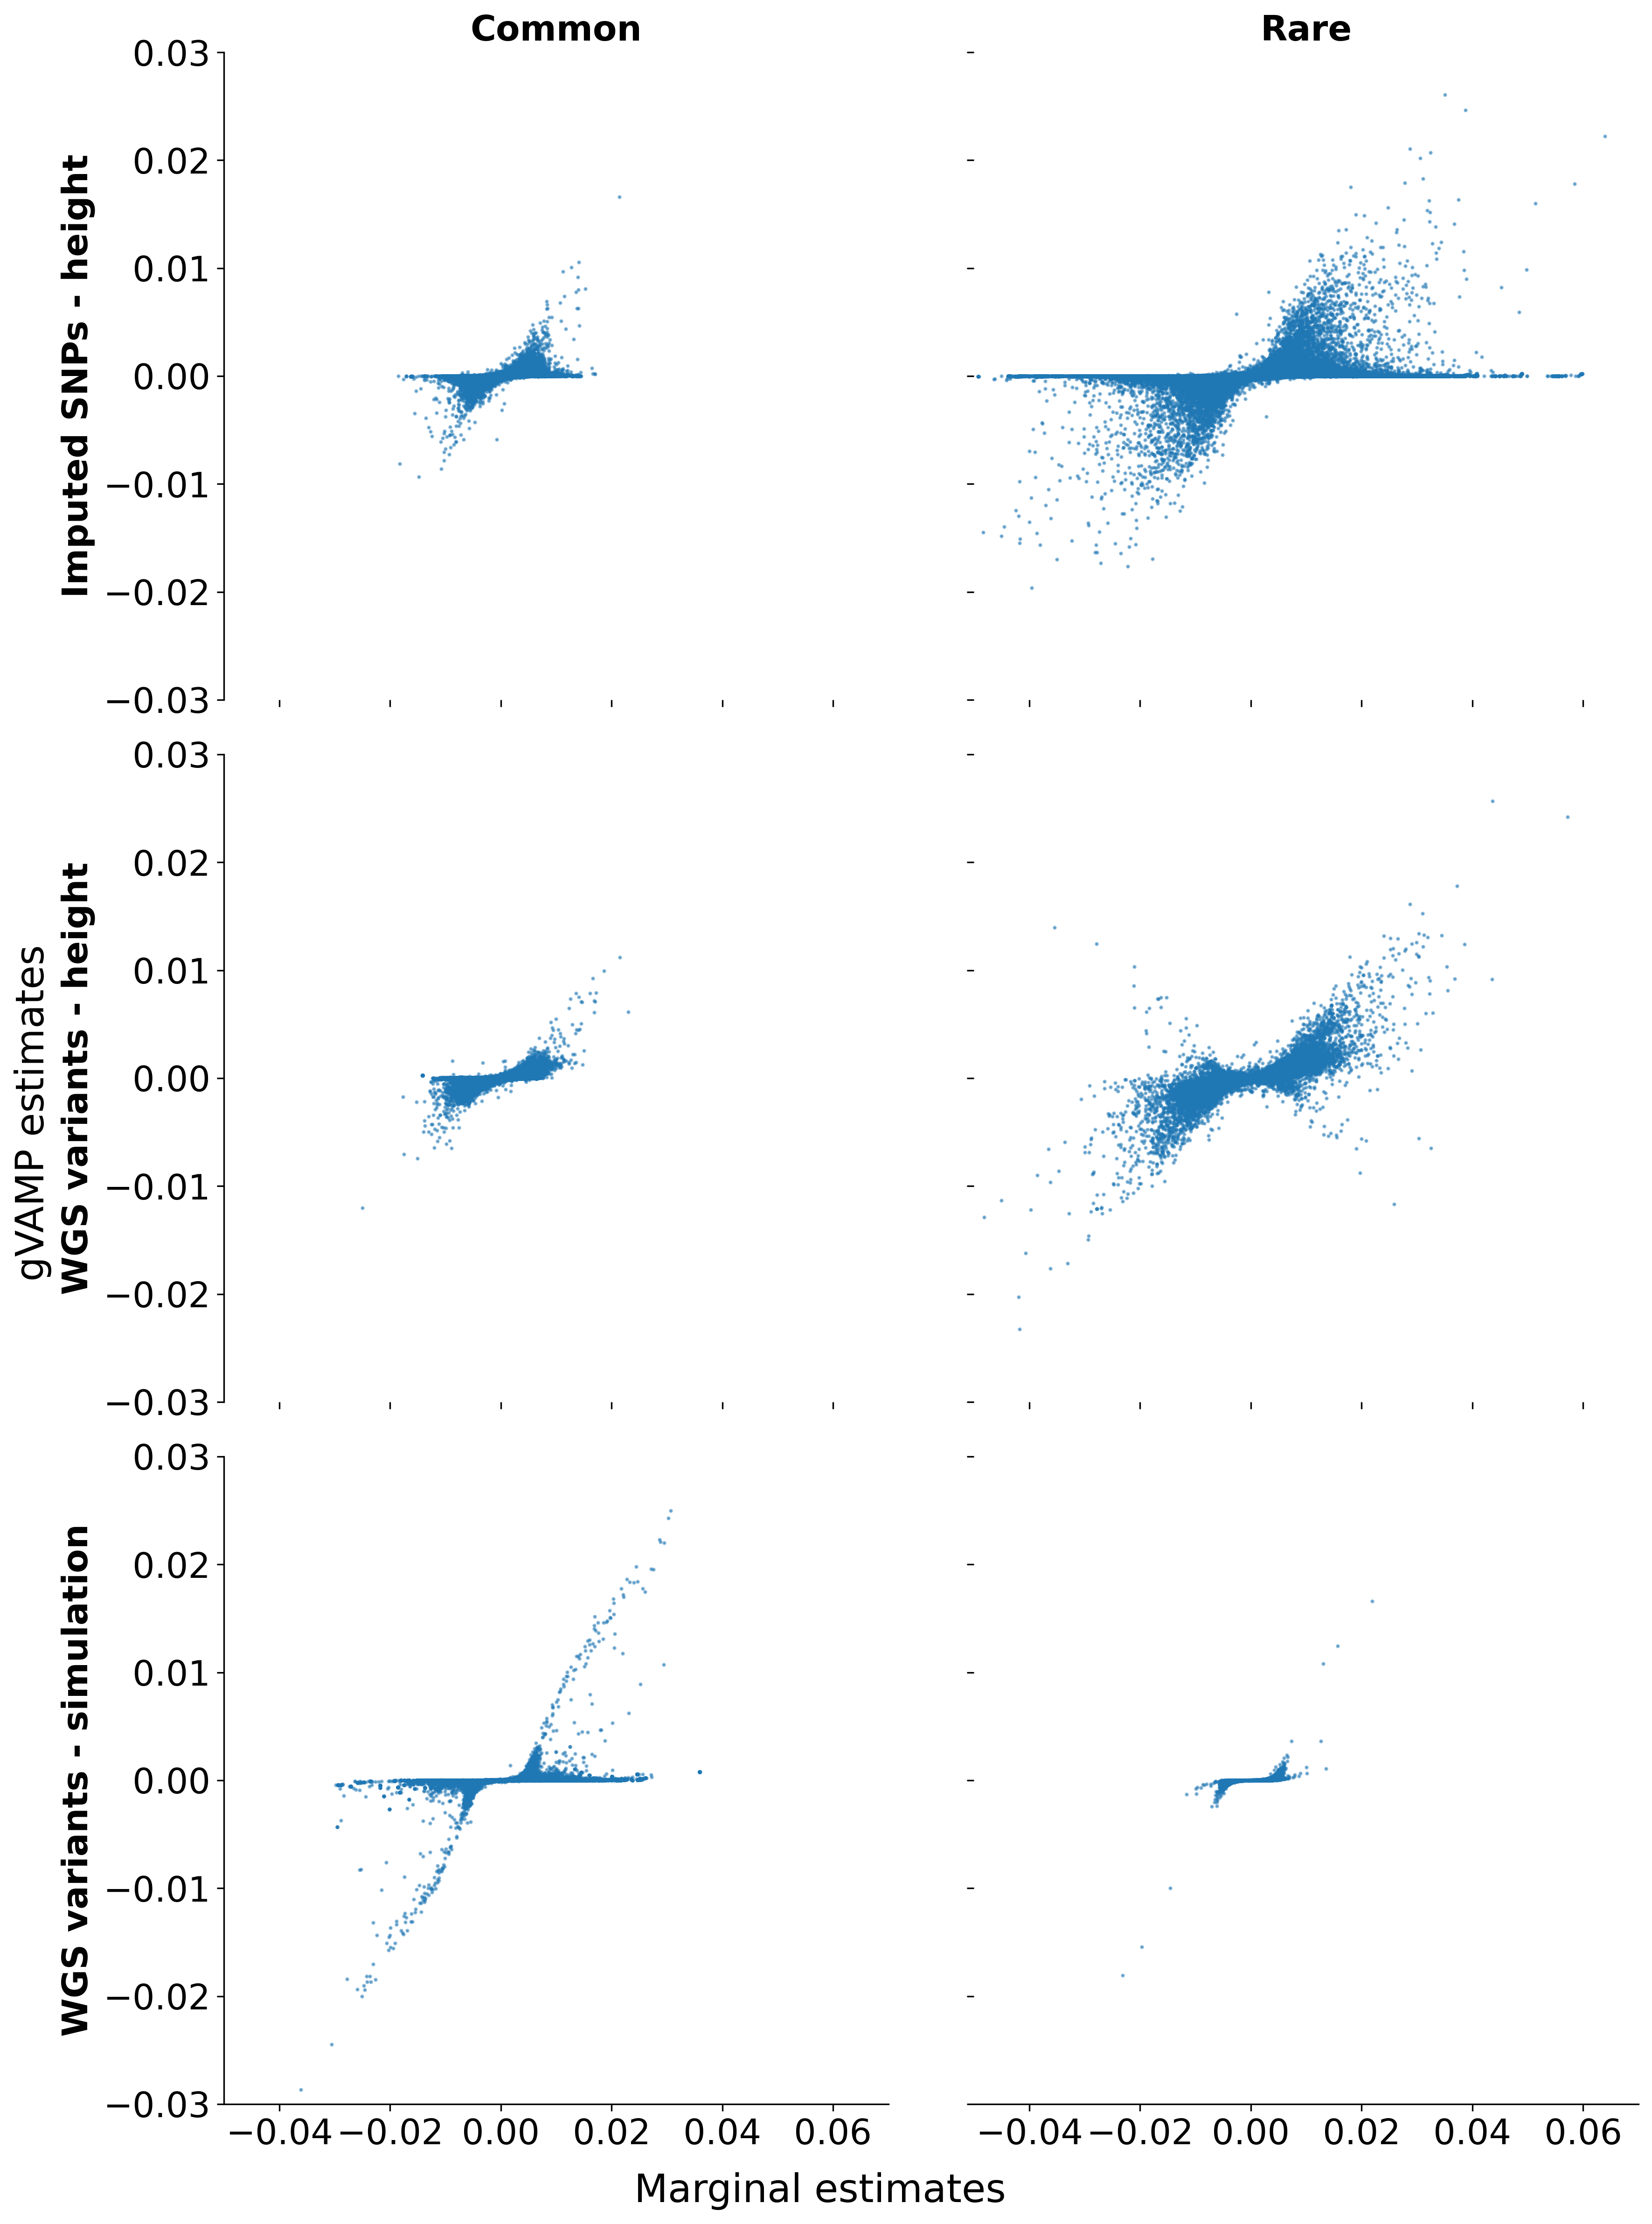
\includegraphics[width=\linewidth]{graphics/gVAMP_figures/v4/FigS9.png}
    \caption[Marginal regression coefficient estimates of the relationship of 16,854,878 whole genome sequence variants with human height, plotted against the regression coefficient values obtained from gVAMP]{\textbf{Marginal regression coefficient estimates of the relationship of 16,854,878 whole genome sequence (WGS) variants with human height, plotted against the regression coefficient values obtained from gVAMP}.}
    \label{fig:figS8}
\end{figure}

\begin{figure}[!t] % the continued legend, at the top of the page after the figure
    \ContinuedFloat
    \captionsetup{labelformat=continued}
    \caption[]{\small "WGS" refers to the gVAMP run on the WGS variants, "Imputed" refers to the gVAMP run on 8,430,446 imputed SNP markers, and "Simulation" gives the same comparison of marginal and gVAMP estimates in setting $a$. The comparison is plotted for common (minor allele frequency, MAF $\ge 1\%$) and rare variants (MAF $< 1\%$).}
\end{figure}

\newpage

\begin{figure}[!htp]
    \centering
    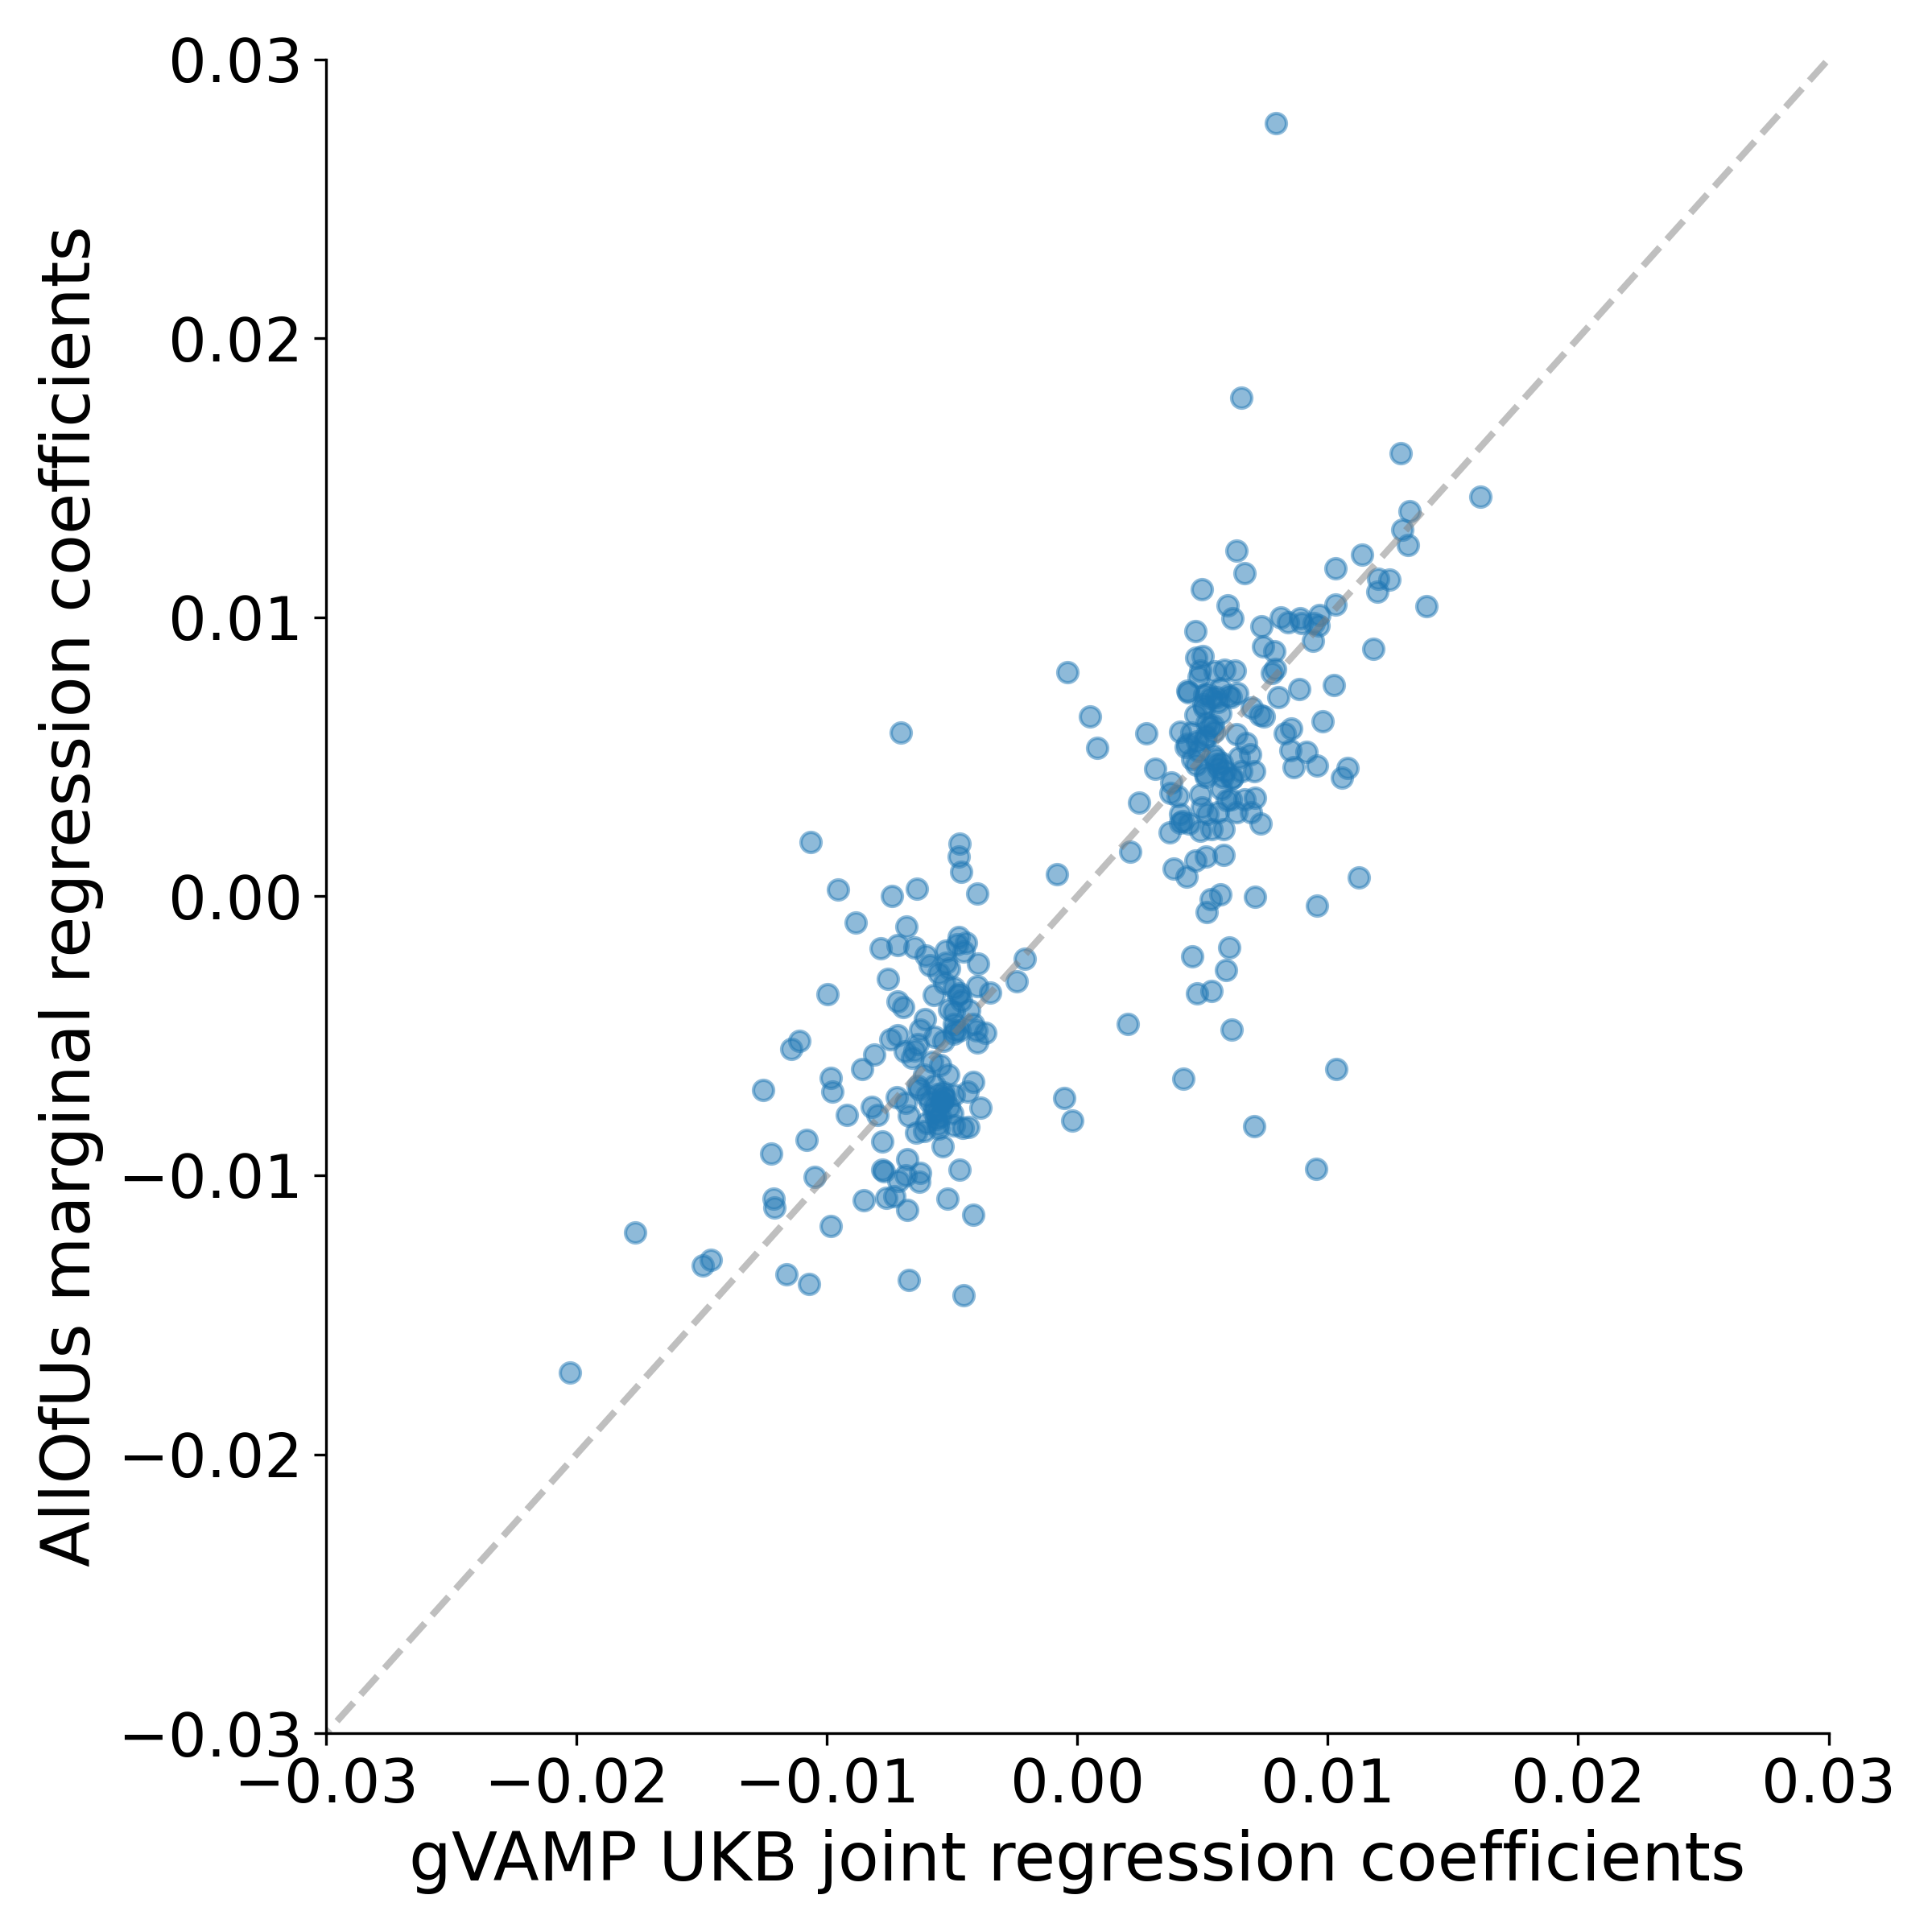
\includegraphics[width=\linewidth]{graphics/gVAMP_figures/v4/FigS10.png}
    \caption[Replication of UK Biobank gVAMP findings in the All of Us dataset]{\textbf{Replication of UK Biobank gVAMP findings in the All of Us dataset.} On the $x$-axis, we plot gVAMP regression coefficient estimates for human height in WGS data discovered at PIP $\geq 0.95$. On the $y$-axis, we plot the marginal regression coefficient estimates of the same SNPs in WGS data in the All of Us dataset, controlling for sex and 16 available PCs. When the major and minor alleles are swapped between two datasets, we change the sign of the effect to match them. The slope of the fitted regression line is $0.8471$.} 
    \label{fig:figS9}
\end{figure}

\newpage

\begin{figure}[!htp]
    \centering
    \includegraphics[width=\linewidth]{graphics/gVAMP_figures/figureS2.png}
    \caption[The variance attributable to gene burden scores calculated from WES data ($y$-axis) shows no relationship to the variance attributable to DNA variants within and around the gene ($x$-axis) estimated from a gVAMP analysis of either 8,430,446 imputed SNP markers or 16,854,878 whole genome sequence variants]{\textbf{The variance attributable to gene burden scores calculated from whole exome sequence (WES) data ($y$-axis) shows no relationship to the variance attributable to DNA variants within and around the gene ($x$-axis) estimated from a gVAMP analysis of either 8,430,446 imputed SNP markers or 16,854,878 whole genome sequence (WGS) variants.}}
    \label{fig:figS10}
\end{figure}


\newpage


\begin{figure}[!htp]
    \centering
    \includegraphics[width=0.88\linewidth]{graphics/gVAMP_figures/old_figs/Figure_S3.png}
    \caption[SNP heritability estimation of GMRM versus gVAMP with different numbers of SNP markers across 13 traits in the UK Biobank]{\textbf{SNP heritability estimation of GMRM versus gVAMP with different numbers of SNP markers across 13 traits in the UK Biobank.} \small Comparison of the proportion of phenotypic variation attributable to 2,174,071 autosomal SNP genetic markers (SNP heritability) estimated by GMRM ($x$-axis) to the SNP heritability estimated by gVAMP ($y$-axis) at either the same 2,174,071 SNPs (red) or 8,430,446 SNP markers (blue). The slope of the lines shows a 1-to-1 relationship of gVAMP to GMRM, but with an average of 3.4\% lower estimate for gVAMP at 2.17M SNPs. Analyzing 8.4M SNPs with gVAMP increases the heritability estimate over GMRM by 3.9\%, which is consistent with an increase in phenotypic variance captured by the full imputed sequence data, as opposed to a selected subset of SNP markers. The dashed grey line gives $y=x$.}
    \label{fig:figS12}
\end{figure}

\newpage


% \section*{Supplementary Note 1}
\refstepcounter{suppnotegvamp}
% \section{Supplementary Note \thesuppnotegvamp}
\section{Prediction accuracy and association testing simulations using imputed UK Biobank data}
\label{supp:note1}

\begin{figure}[!htp]
    \centering   
    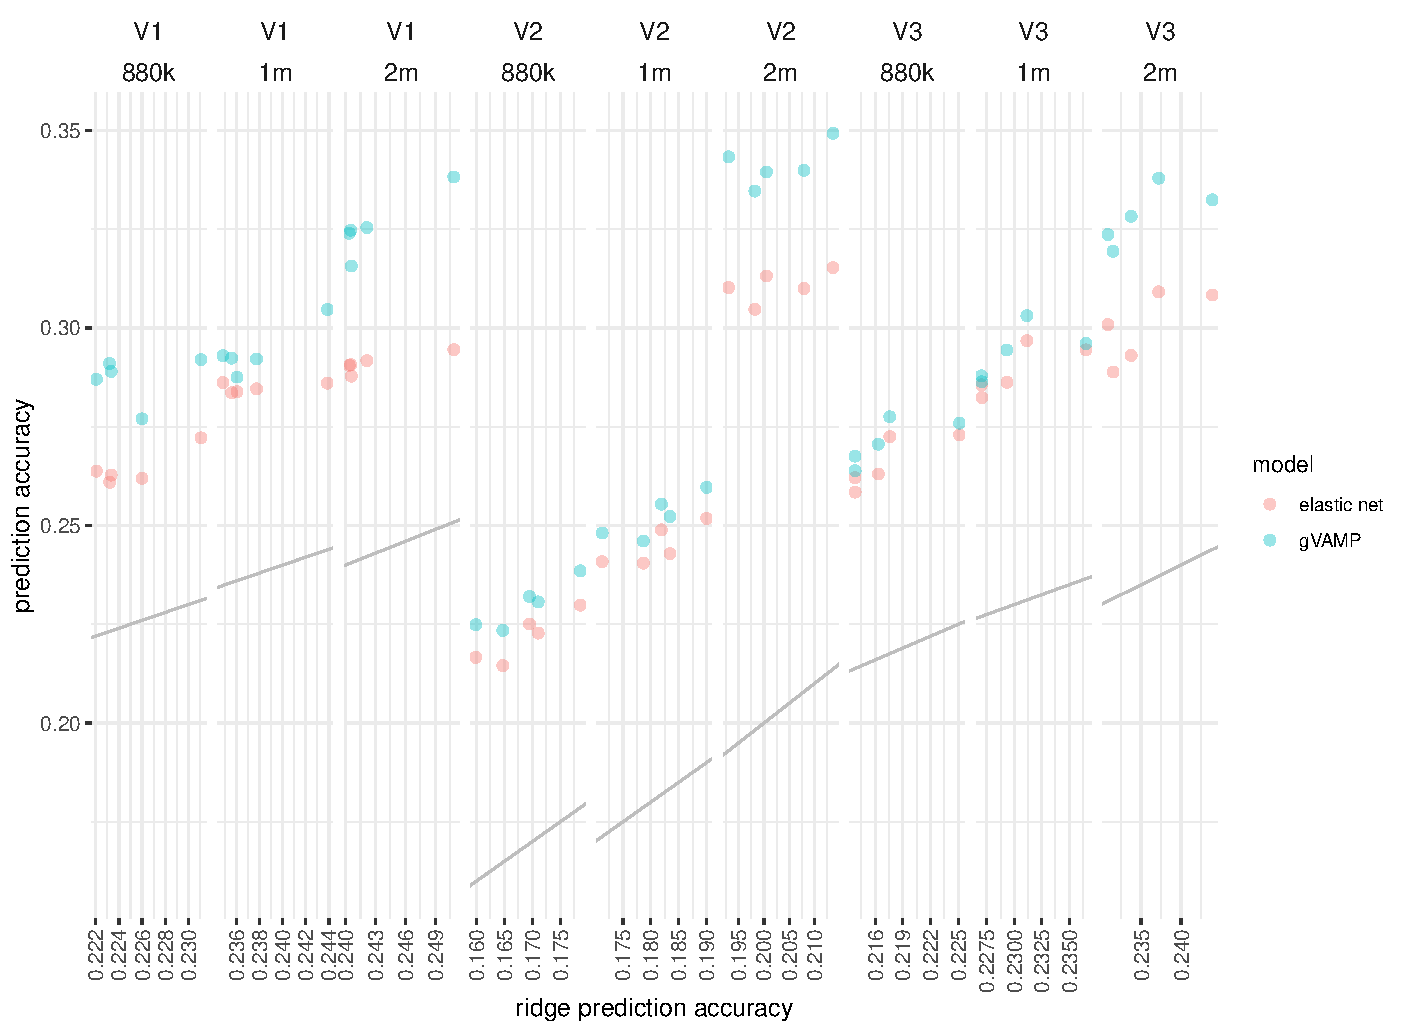
\includegraphics[width=\linewidth]{graphics/gVAMP_figures/Fig_SN1.pdf}
    \caption[Simulation study of out-of-sample prediction accuracy in UK Biobank imputed genotype data]{\textbf{Simulation study of out-of-sample prediction accuracy in UK Biobank imputed genotype data.} \small{We compare out-of-sample prediction accuracy ($y$-axis) for polygenic risk scores (PRS) created at different sets of markers ("880k" = 887,060, "1m" = 1,410,525, "2m" = 2,174,071 SNPs) from gVAMP (blue) and an elastic net model implemented in the LDAK software (red), as compared to the prediction accuracy obtained at the same sets of SNPs from a ridge regression model implemented in the LDAK software ($x$-axis). Grey lines give the 1:1 line. Comparisons are made across three settings: "V1" where 40,000 causal variants are randomly selected from 8,430,446 SNP markers and effects are drawn from a Gaussian, "V2" where 40,000 causal variants are randomly selected from 8,430,446 SNP markers, with effects that have a power relationship to the minor allele frequency of -0.5, and "V3" where 40,000 causal variants are randomly selected from 8,430,446 SNP markers, with effects drawn from an elastic net distribution.}}
    \label{fig:figSN1}
\end{figure}

\begin{figure}[!htp]
    \centering   
    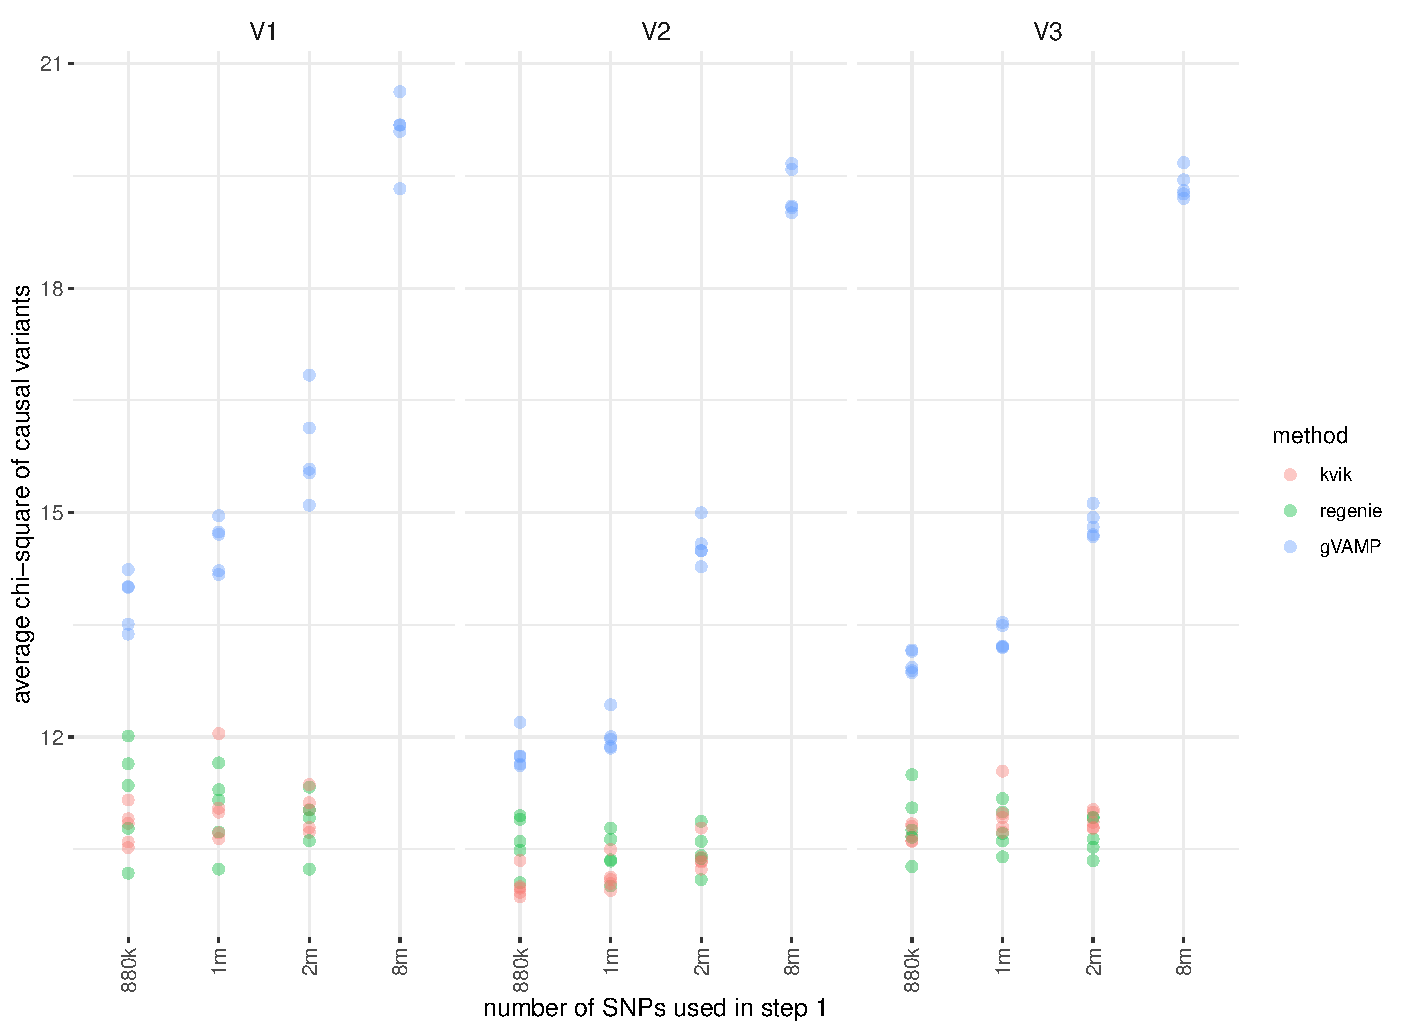
\includegraphics[width=\linewidth]{graphics/gVAMP_figures/Fig_SN2.pdf}
    \caption[Simulation study of power for mixed linear model leave-one-chromosome out association testing in UK Biobank imputed genotype data]{\textbf{Simulation study of power for mixed linear model leave-one-chromosome out association testing in UK Biobank imputed genotype data.} \small{We compare the average chi-squared value at the causal variants ($y$-axis) for leave-one-chromosome-out association testing (LOCO) when the first step LOCO predictors are created at different sets of markers ("880k" = 887,060, "1m" = 1,410,525, "2m" = 2,174,071 SNPs) from gVAMP (blue), an elastic net model implemented in the LDAK software (red), and Regenie (green). Comparisons are made across three settings: "V1" where 40,000 causal variants are randomly selected from 8,430,446 SNP markers and effects are drawn from a Gaussian, "V2" where 40,000 causal variants are randomly selected from 8,430,446 SNP markers, with effects that have a power relationship to the minor allele frequency of -0.5, and "V3" where 40,000 causal variants are randomly selected from 8,430,446 SNP markers, with effects drawn from an elastic net distribution.}}
    \label{fig:figSN2}
\end{figure}

\begin{figure}[!htp]
    \centering   
    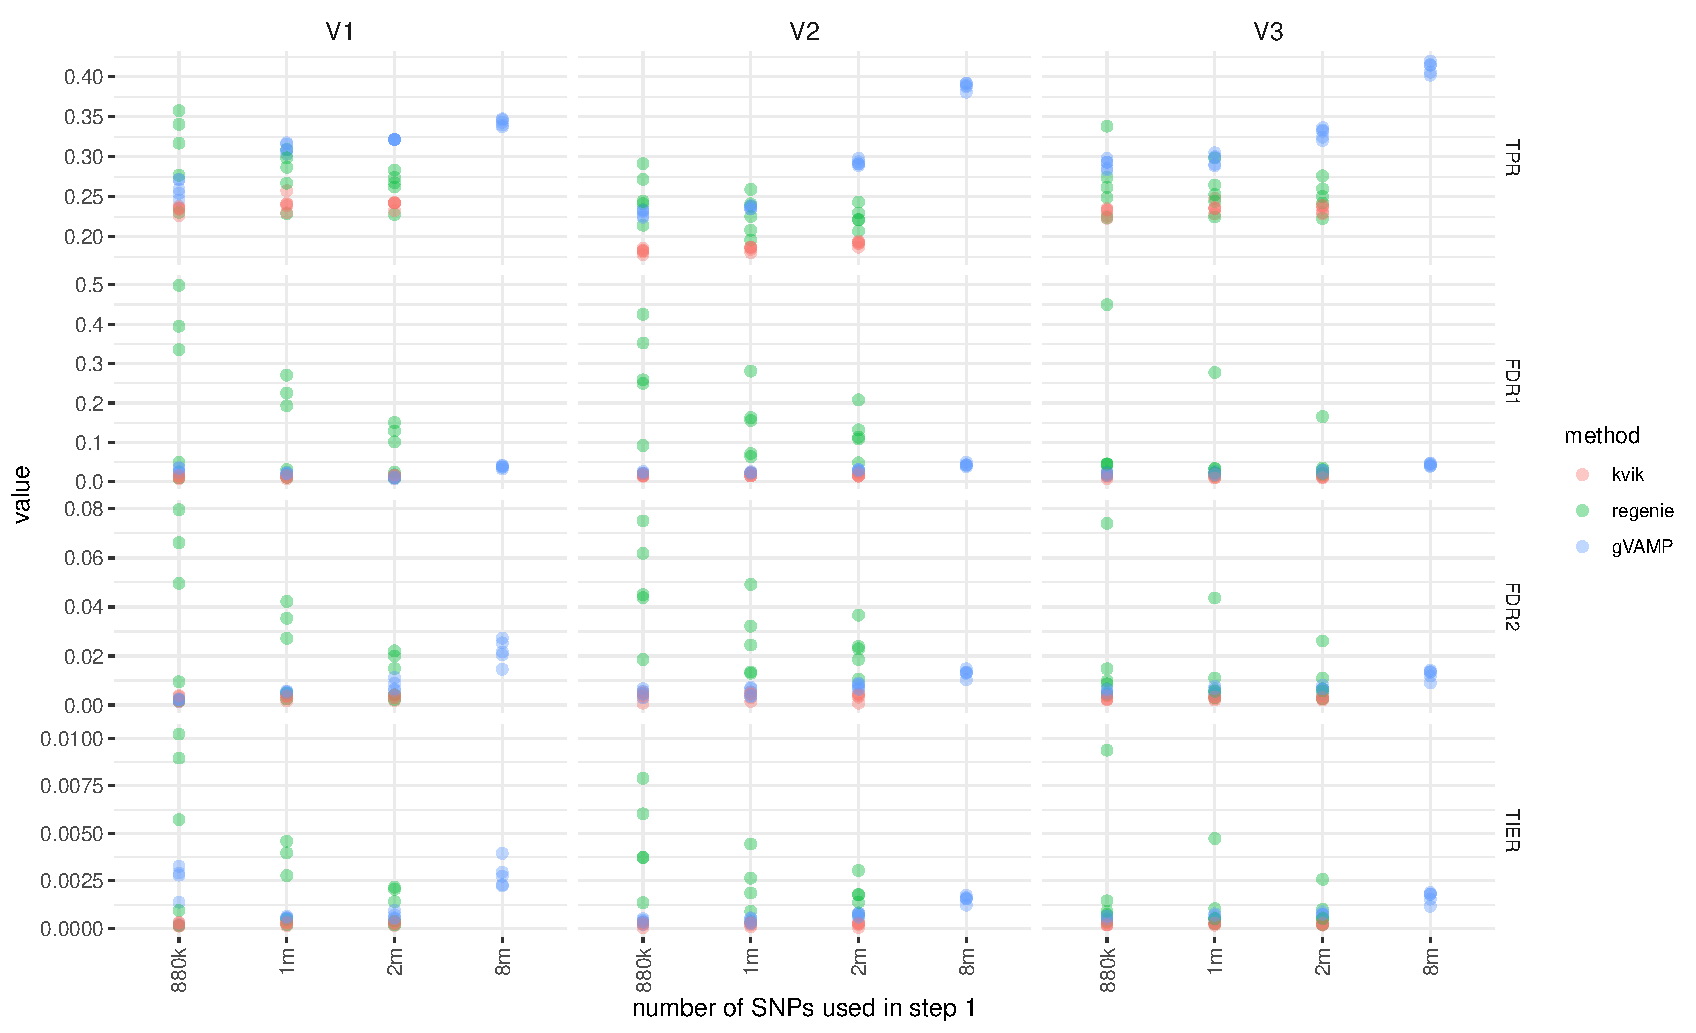
\includegraphics[width=\linewidth]{graphics/gVAMP_figures/Fig_SN3.pdf}
    \caption[Simulation study of true positive rate (TPR), false discovery rate (FDR) and type-I error for mixed linear model leave-one-chromosome out association testing in UK Biobank imputed genotype data]{\textbf{Simulation study of true positive rate (TPR), false discovery rate (FDR) and type-I error for mixed linear model leave-one-chromosome out association testing in UK Biobank imputed genotype data.} \small{We compare performance of leave-one-chromosome-out association testing (LOCO) when the first step LOCO predictors are created at different sets of markers ("880k" = 887,060, "1m" = 1,410,525, "2m" = 2,174,071 SNPs) from gVAMP (blue), an elastic net model implemented in the LDAK software (red), and Regenie (green). Comparisons are made across three settings: "V1" where 40,000 causal variants are randomly selected from 8,430,446 SNP markers and effects are drawn from a Gaussian, "V2" where 40,000 causal variants are randomly selected from 8,430,446 SNP markers, with effects that have a power relationship to the minor allele frequency of -0.5, and "V3" where 40,000 causal variants are randomly selected from 8,430,446 SNP markers, with effects drawn from an elastic net distribution. For each 1Mb window that contains an identified genome-wide significant association, we then ask if the identified variants are correlated (squared correlation $\geq 0.01$) to a causal variant: if so, we classify the window as a true positive; otherwise, we classify it as a false positive. The true positive rate is calculated as the number of true positive 1Mb windows divided by the total number of simulated causal variants, and it is also known as the recall, or sensitivity, reflecting the power of a statistical test.}}
    \label{fig:figSN3}
\end{figure}

\begin{figure}[!t] % the continued legend, at the top of the page after the figure
    \ContinuedFloat
    \captionsetup{labelformat=continued}
    \caption[]{\small{We provide two measures of the false discovery rate: FDR1 is calculated as the number of false positive 1Mb windows divided by the number of 1Mb windows that contain genome-wide significant associations, and it is a measure of the proportion of independent discoveries that are false. FDR2 is calculated as the total number of false positive SNPs (squared correlation $\leq 0.01$ with a causal variant) identified divided by the total number of identified genome-wide significant associations. We calculate the type-I error rate (TIER) as the number of SNPs with no correlation to a causal variant (squared correlation $\leq 0.01$ with a causal variant) that pass the Bonferroni genome-wide significance testing threshold divided by the total number of SNPs that have no correlation to a causal variant (squared correlation $\leq 0.01$ with a causal variant).}}
\end{figure}

\begin{figure}[!htp]
    \centering   
    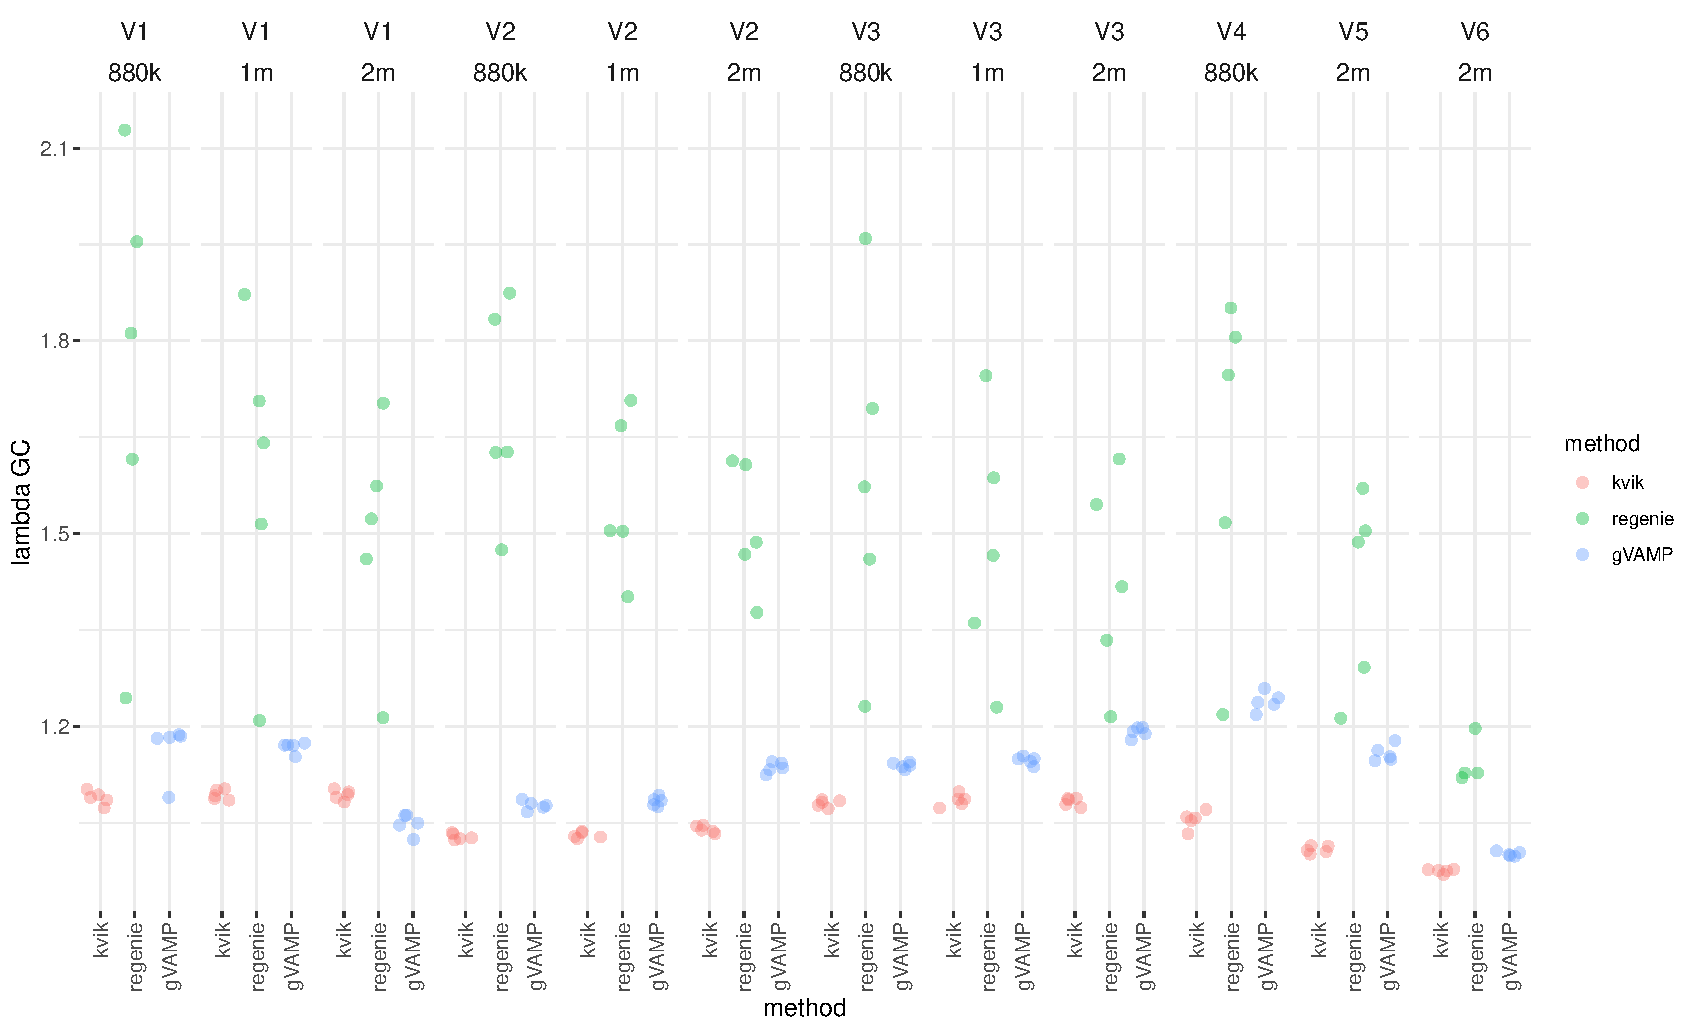
\includegraphics[width=\linewidth]{graphics/gVAMP_figures/Fig_SN7.pdf}
    \caption[Simulation study of lambda GC ($\lambda_{GC}$) values of mixed linear model leave-one-chromosome out association testing in UK Biobank imputed genotype data]{\textbf{Simulation study of lambda GC ($\lambda_{GC}$) values of mixed linear model leave-one-chromosome out association testing in UK Biobank imputed genotype data.} \small{We compare performance of leave-one-chromosome-out association testing (LOCO) when the first step LOCO predictors are created at different sets of markers, from gVAMP (blue), an elastic net model implemented in the LDAK software (red), and Regenie (green). Comparisons are made across six settings: "V1" where 40,000 causal variants are randomly selected from 8,430,446 SNP markers and effects are drawn from a Gaussian, "V2" where 40,000 causal variants are randomly selected from 8,430,446 SNP markers, with effects that have a power relationship to the minor allele frequency of -0.5, "V3" where 40,000 causal variants are randomly selected from 8,430,446 SNP markers, with effects drawn from an elastic net distribution, "V4" where 40,000 causal variants are randomly selected from 887,060 SNPs, with effects that contribute 50\% to the phenotypic variance and have a power relationship to the minor allele frequency of -0.5, "V5" where 40,000 causal variants are randomly selected from 2,174,071 SNPs, with effects that contribute 50\% to the phenotypic variance and have a power relationship to the minor allele frequency of -0.5, and "V6" where 5,000 causal variant effects are randomly selected from 2,174,071 SNPs, with effects that contribute 25\% to the phenotypic variance and have a power relationship to the minor allele frequency of -0.5. For each replicate, we calculate the ratio of the median chi-square to the expected median chi-square values ($\lambda_{GC}$).}}
    \label{fig:figSN4}
\end{figure}


\begin{figure}[!htp]
    \centering   
    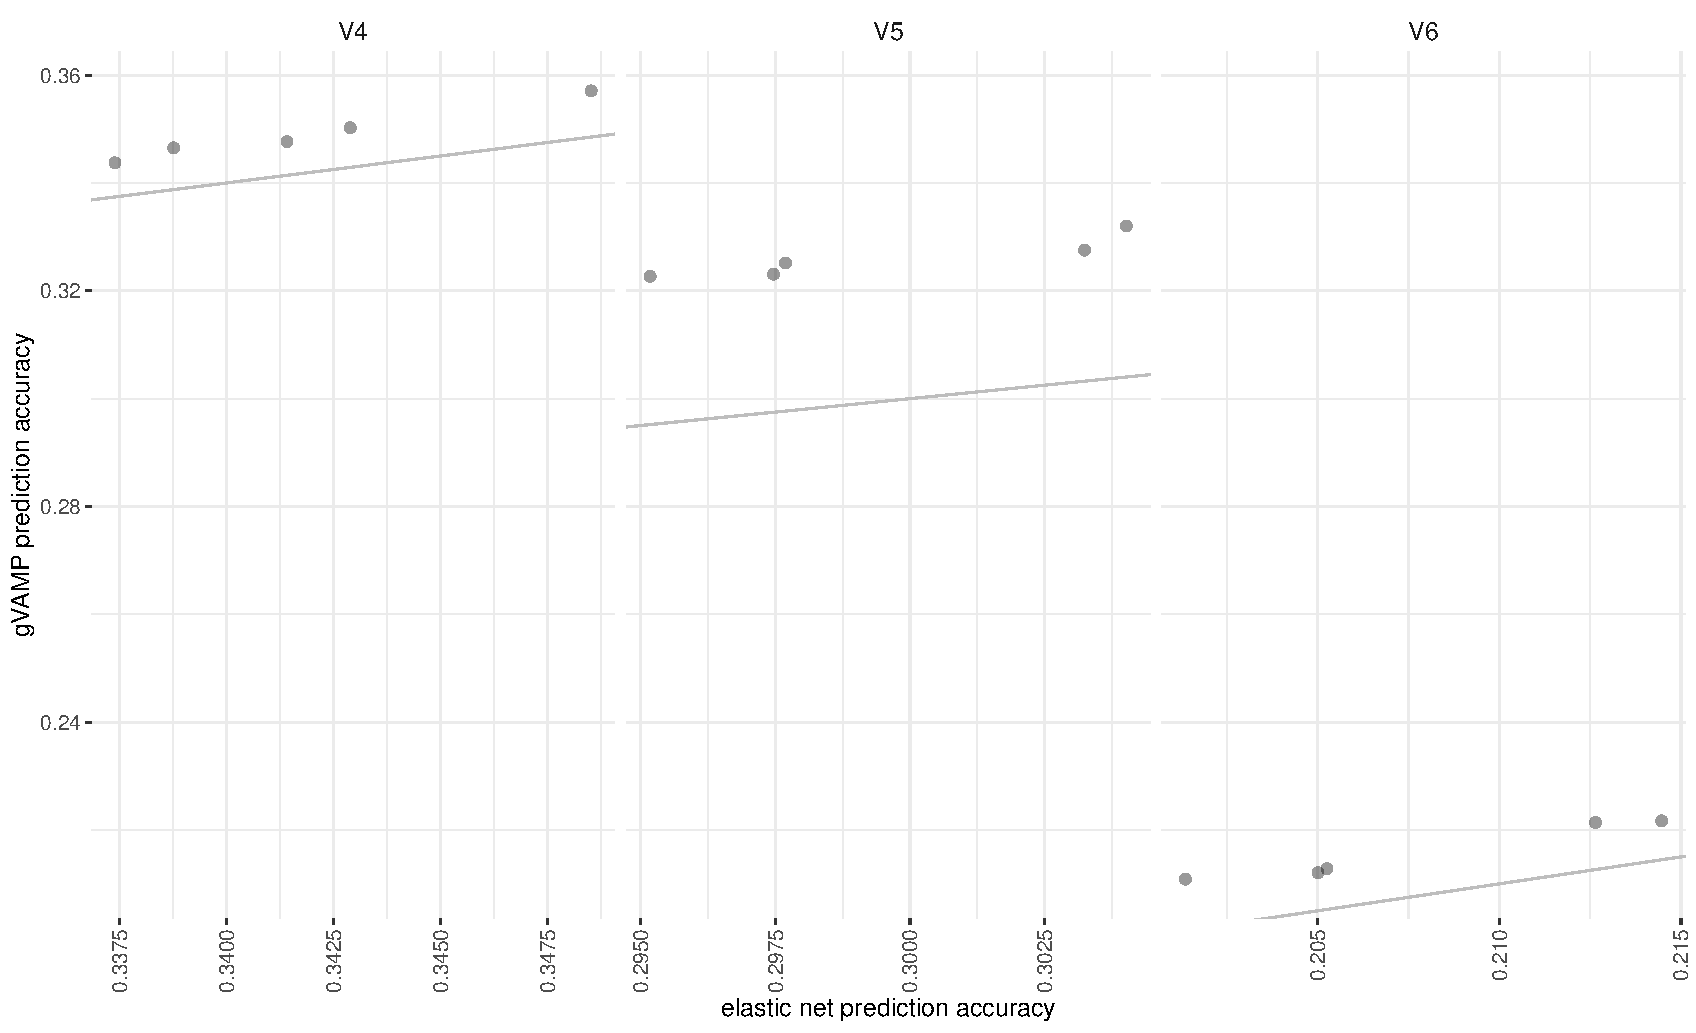
\includegraphics[width=\linewidth]{graphics/gVAMP_figures/Fig_SN4.pdf}
    \caption[Simulation study of out-of-sample prediction accuracy in UK Biobank imputed genotype data]{\textbf{Simulation study of out-of-sample prediction accuracy in UK Biobank imputed genotype data.} \small{We compare out-of-sample prediction accuracy ($y$-axis) for polygenic risk scores (PRS) created at different sets of markers from gVAMP and an elastic net model implemented in the LDAK software. Grey lines give the 1:1 line. Comparisons are made across three settings: "V4" where 40,000 causal variants are randomly selected from 887,060 SNPs, with effects that contribute 50\% to the phenotypic variance and have a power relationship to the minor allele frequency of -0.5, "V5" where 40,000 causal variants are randomly selected from 2,174,071 SNPs, with effects that contribute 50\% to the phenotypic variance and have a power relationship to the minor allele frequency of -0.5, and "V6" where 5,000 causal variant effects are randomly selected from 2,174,071 SNPs, with effects that contribute 25\% to the phenotypic variance and have a power relationship to the minor allele frequency of -0.5.}}
    \label{fig:figSN5}
\end{figure}

\begin{figure}[!htp]
    \centering   
    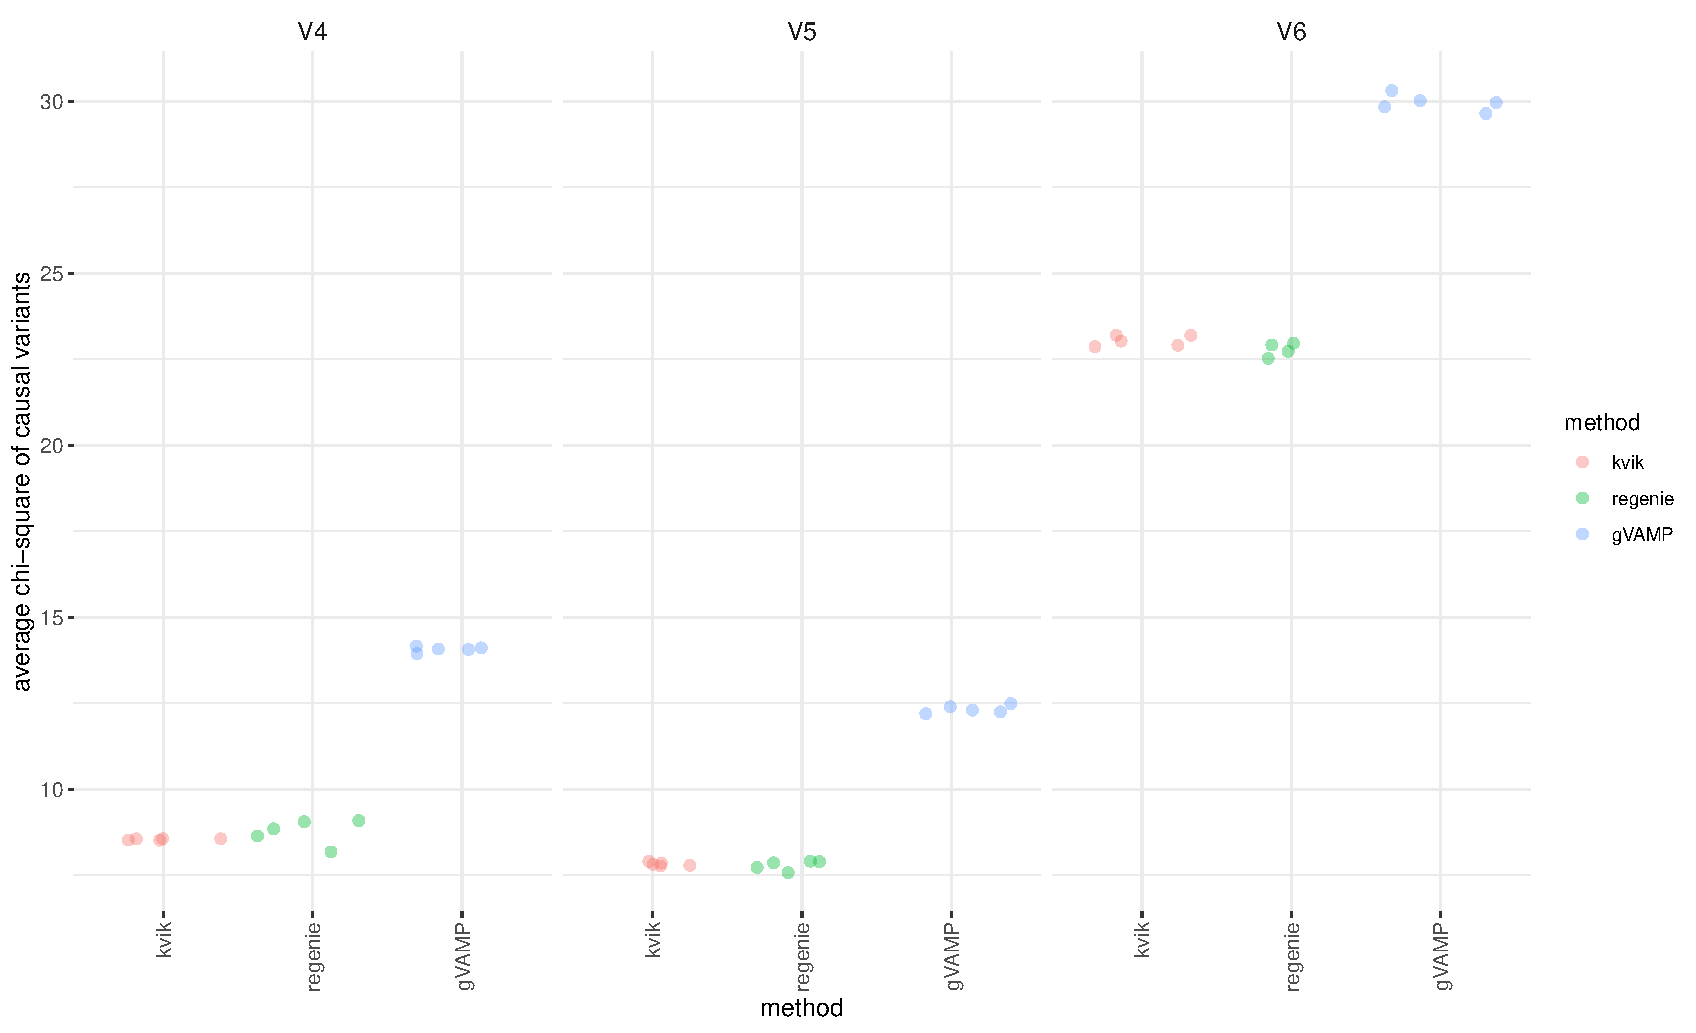
\includegraphics[width=\linewidth]{graphics/gVAMP_figures/Fig_SN5.pdf}
    \caption[Simulation study of power for mixed linear model leave-one-chromosome out association testing in UK Biobank imputed genotype data]{\textbf{Simulation study of power for mixed linear model leave-one-chromosome out association testing in UK Biobank imputed genotype data.} \small{We compare the average chi-squared value at the causal variants ($y$-axis) for leave-one-chromosome-out association testing (LOCO) when the first step LOCO predictors are created at different sets of markers, from gVAMP (blue), an elastic net model implemented in the LDAK software (red), and Regenie (green). Comparisons are made across three settings: "V4" where 40,000 causal variants are randomly selected from 887,060 SNPs, with effects that contribute 50\% to the phenotypic variance and have a power relationship to the minor allele frequency of -0.5, "V5" where 40,000 causal variants are randomly selected from 2,174,071 SNPs, with effects that contribute 50\% to the phenotypic variance and have a power relationship to the minor allele frequency of -0.5, and "V6" where 5,000 causal variant effects are randomly selected from 2,174,071 SNPs, with effects that contribute 25\% to the phenotypic variance and have a power relationship to the minor allele frequency of -0.5.}}
    \label{fig:figSN6}
\end{figure}

\begin{figure}[!htp]
    \centering   
    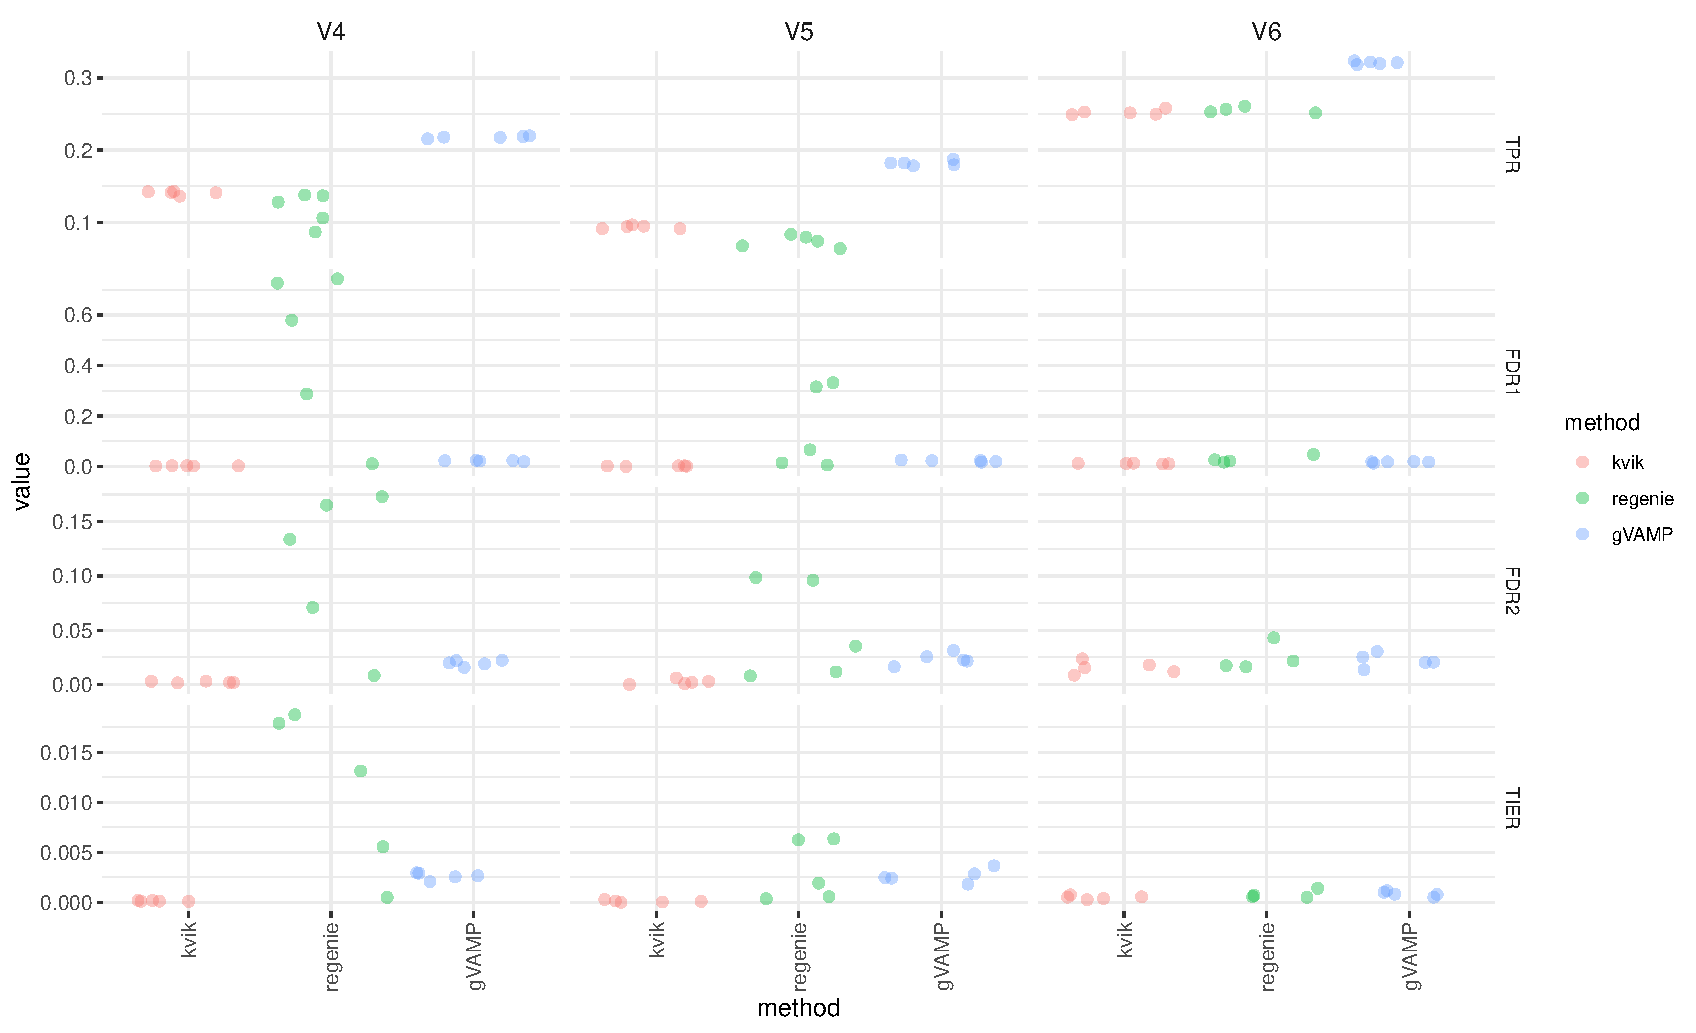
\includegraphics[width=\linewidth]{graphics/gVAMP_figures/Fig_SN6.pdf}
    \caption[Simulation study of true positive rate (TPR), false discovery rate (FDR) and type-I error for mixed linear model leave-one-chromosome out association testing in UK Biobank imputed genotype data]{\textbf{Simulation study of true positive rate (TPR), false discovery rate (FDR) and type-I error for mixed linear model leave-one-chromosome out association testing in UK Biobank imputed genotype data.} \small{We compare performance of leave-one-chromosome-out association testing (LOCO) when the first step LOCO predictors are created at different sets of markers, from gVAMP (blue), an elastic net model implemented in the LDAK software (red), and Regenie (green). Comparisons are made across three settings: "V4" where 40,000 causal variants are randomly selected from 887,060 SNPs, with effects that contribute 50\% to the phenotypic variance and have a power relationship to the minor allele frequency of -0.5, "V5" where 40,000 causal variants are randomly selected from 2,174,071 SNPs, with effects that contribute 50\% to the phenotypic variance and have a power relationship to the minor allele frequency of -0.5, and "V6" where 5,000 causal variant effects are randomly selected from 2,174,071 SNPs, with effects that contribute 25\% to the phenotypic variance and have a power relationship to the minor allele frequency of -0.5. For each 1Mb window that contains an identified genome-wide significant association, we then ask if the identified variants are correlated (squared correlation $\geq 0.01$) to a causal variant: if so, we classify the window as a true positive; otherwise, we classify it as a false positive. The true positive rate is calculated as the number of true positive 1Mb windows divided by the total number of simulated causal variants, and it is also known as the recall, or sensitivity, reflecting the power of a statistical test.}}
    \label{fig:figSN7}
\end{figure}

\begin{figure}[!t] % the continued legend, at the top of the page after the figure
    \ContinuedFloat
    \captionsetup{labelformat=continued}
    \caption[]{\small{We provide two measures of the false discovery rate: FDR1 is calculated as the number of false positive 1Mb windows divided by the number of 1Mb windows that contain genome-wide significant associations, and it is a measure of the proportion of independent discoveries that are false. FDR2 is calculated as the total number of false positive SNPs (squared correlation $\leq 0.01$ with a causal variant) identified divided by the total number of identified genome-wide significant associations. We calculate the type-I error rate (TIER) as the number of SNPs with no correlation to a causal variant (squared correlation $\leq 0.01$ with a causal variant) that pass the Bonferroni genome-wide significance testing threshold divided by the total number of SNPs that have no correlation to a causal variant (squared correlation $\leq 0.01$ with a causal variant).}}
\end{figure}


\begin{figure}[!htp]
    \centering
    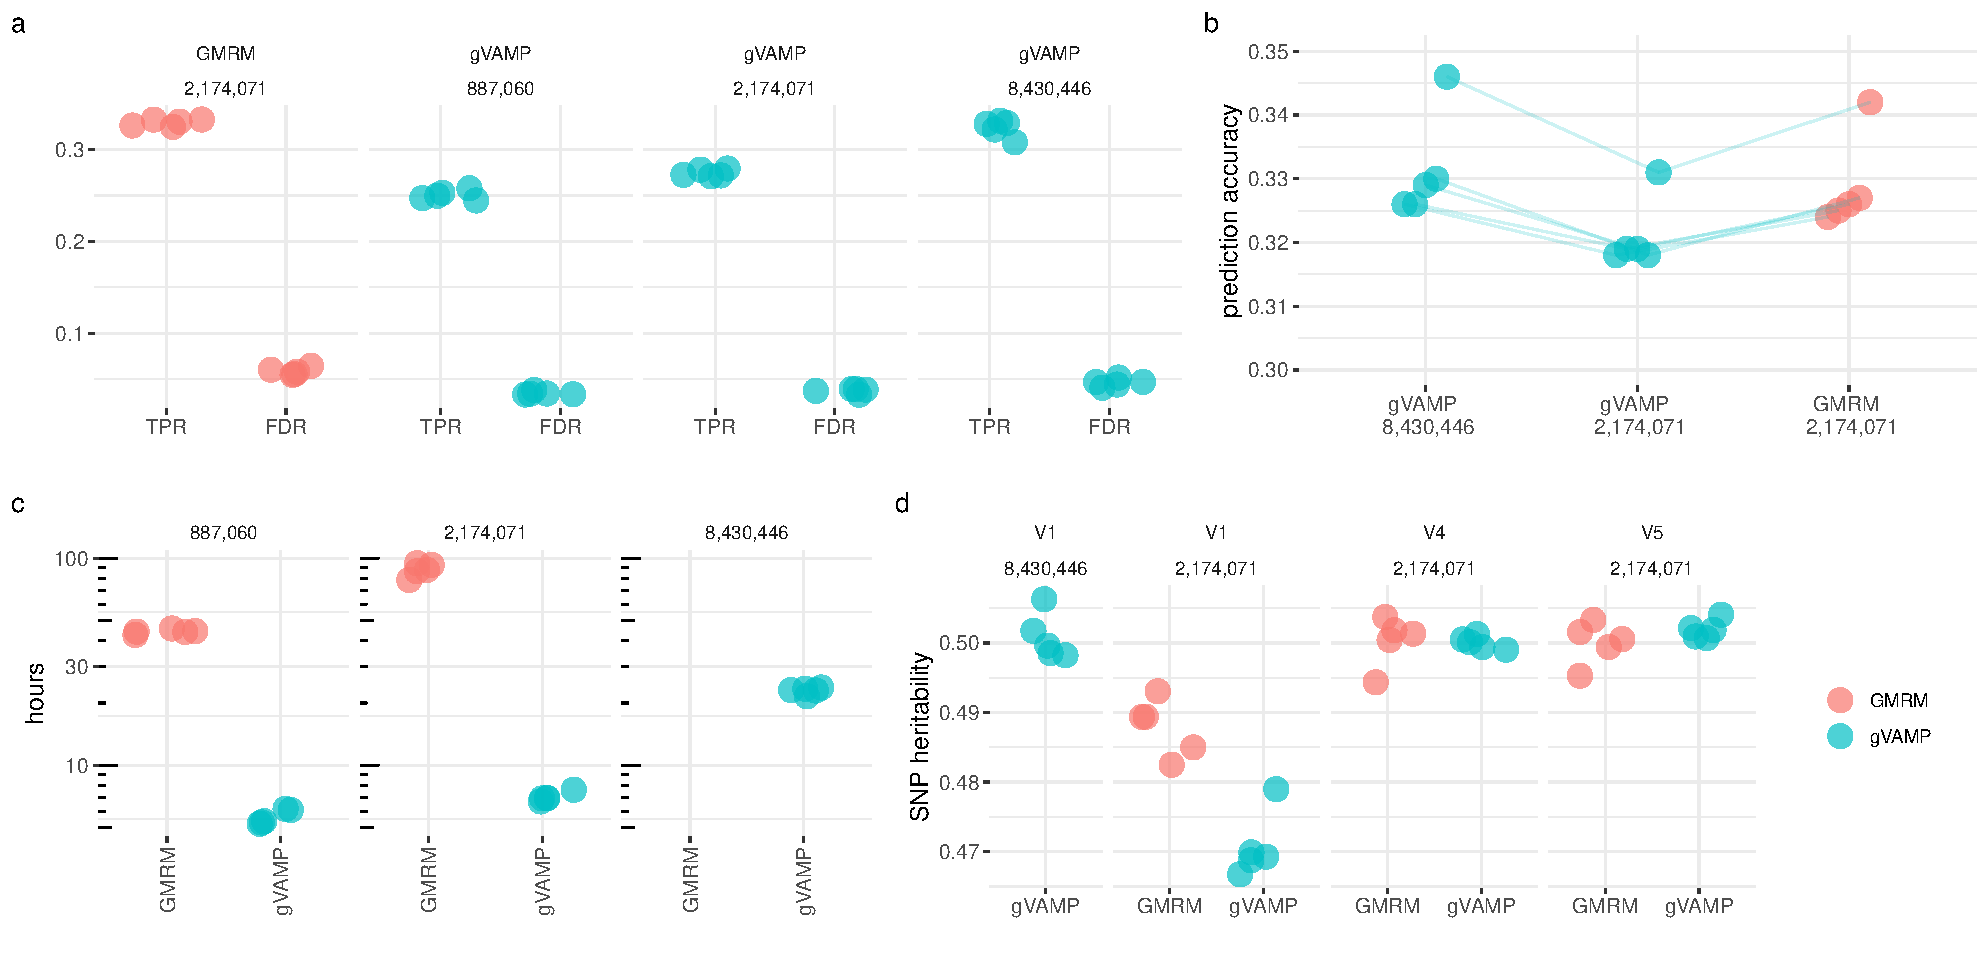
\includegraphics[width=\linewidth]{graphics/gVAMP_figures/gVAMP_GMRM.pdf}
    \caption[Comparison of MCMC Gibbs sampling algorithm GMRM to gVAMP in an imputed UK Biobank data simulation study]{\textbf{Comparison of MCMC Gibbs sampling algorithm GMRM to gVAMP in an imputed UK Biobank data simulation study.} \small For a simulation setting where 40,000 causal variants are randomly selected from 8,430,446 SNP markers and effects are drawn from a Gaussian ("V1"), in \emph{(a)}, we show results from standard leave-one-chromosome-out (LOCO) association testing where we select either all markers, 2,174,071 markers, or 887,060 markers for the first stage and then use all markers for the second stage LOCO testing. GMRM utilises 2,174,071 markers, whilst gVAMP can utilise the full range. We calculate the true positive rate (TPR) and the false discovery rate (FDR) and find that the FDR is well controlled at 5\% or less for both gVAMP and GMRM. For \emph{(b)}, we compare out-of-sample prediction accuracy for polygenic risk scores created at different sets of markers from gVAMP (8,430,446 and 2,174,071) and GMRM (2,174,071). \emph{(c)} gives the run time in hours for the first stage analysis of gVAMP and GMRM, across different marker sets using 50 CPU from a single compute node. \emph{(d)} gives a comparison of the proportion of phenotypic variation attributable to either 8,430,446 or a subset of 2,174,071 autosomal single nucleotide polymorphism (SNP) genetic markers (SNP heritability) estimated by GMRM and gVAMP. We consider three simulation scenarios: "V1" where 40,000 causal variants are randomly selected from 8,430,446 SNP markers and effects are drawn from a Gaussian, "V4" where 40,000 causal variants are randomly selected from 887,060 SNPs, with effects that contribute 50\% to the phenotypic variance and have a power relationship to the minor allele frequency of -0.5, "V5" where 40,000 causal variants are randomly selected from 2,174,071 SNPs, with effects that contribute 50\% to the phenotypic variance and have a power relationship to the minor allele frequency of -0.5. Points give the posterior means for GMRM and the convergence of gVAMP from five simulation replicates. Analysing 8,430,446 SNPs with gVAMP increases the heritability estimate over GMRM. This is consistent with an increase in phenotypic variance captured by the full imputed sequence data, as opposed to analyzing a selected subset of SNP markers, in which case gVAMP estimates are lower than those obtained from GMRM. Given the same data containing all the causal variants, the algorithms perform similarly irrespective of the underlying effect size distributions (``V4'' and ``V5'').}
    \label{fig:figSN8}
\end{figure}

\begin{figure}[!htp]
    \centering
    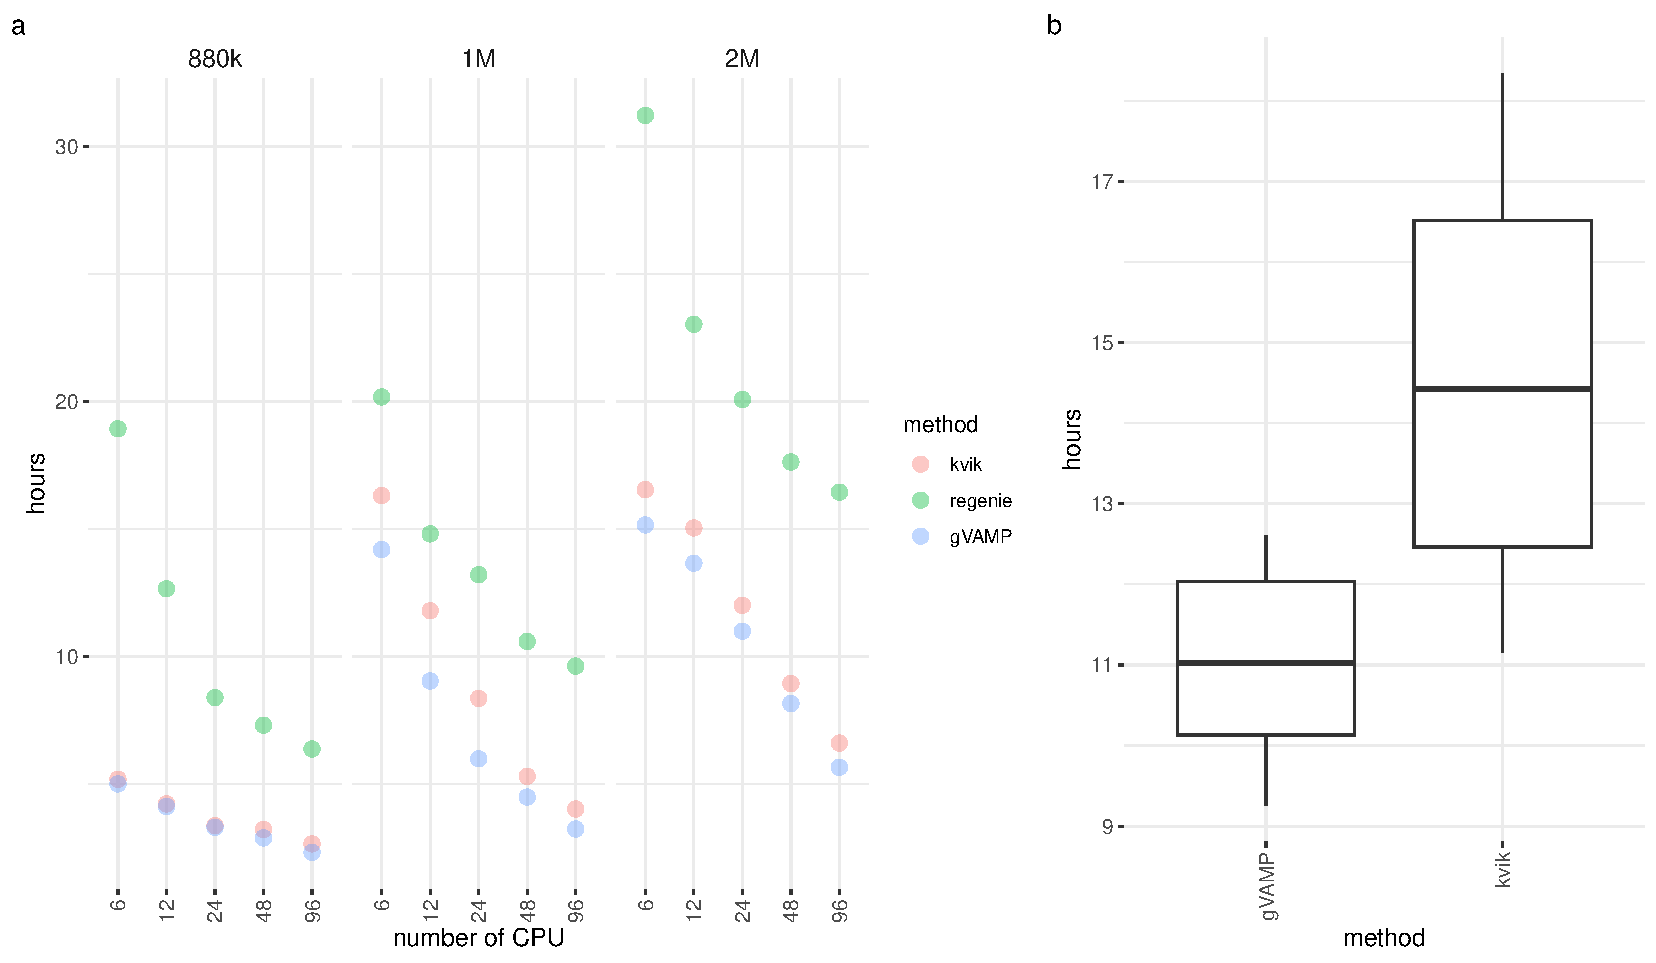
\includegraphics[width=\linewidth]{graphics/gVAMP_figures/timing_plot.pdf}
    \caption[Timing comparison of LDAK elastic net prediction model and gVAMP in an imputed UK Biobank data simulation study and across 13 UK Biobank traits]{\textbf{Timing comparison of LDAK elastic net prediction model and gVAMP in (a) an imputed UK Biobank data simulation study and (b) across 13 UK Biobank traits.} \small \emph{(a)} For simulation setting "V3" where 40,000 causal variants are randomly selected from 8,430,446 SNP markers, with effects drawn from an elastic net distribution, we show the total run time of the algorithms when run on different numbers of imputed SNP markers and given different numbers of CPU resources from a single AMD EPYC 7763 (64 cores, 2.45 GHz base-frequency) compute machine. \emph{(b)} A boxplot of the run time of the algorithms when run on $13$ different UK Biobank traits and 2,174,071 SNPs, when given 60 CPU. Training data sample size is given in Table \ref{table:tableS2} for each trait.}
    \label{fig:figSN9}
\end{figure}

\subsection*{Simulation study in imputed SNP data}
To support our empirical analyses we also conduct a simulation study in imputed SNP data using the 8,430,446 UK Biobank genetic marker data with 414,055 individuals. Our WGS simulation focused on variable selection of exact SNP positions and thus to give power to select variables and to enable clear comparisons of fine-mapping methods (where the objective was the selection of a single variable out of a segment) we simulated only 500 or 1000 causal variables on chromosomes 11-15. Here, we sought to simulate the other extreme of a very highly polygenic genetic basis and thus we randomly sample 40,000 causal variants genome-wide (effectively 4 times the density of causal variants simulated in the WGS simulation). We then simulate three scenarios. First, in \emph{V1}, we allocate effect sizes from a Gaussian with mean zero and variance $0.5/40000$, where $0.5$ is the proportion of variance attributable to the SNP markers. Multiplying the simulated SNP effects by normalized values of the 40,000 causal markers, gives a vector of genetic values of length $N=414055$ with variance 0.5. To this we add a vector of noise, drawn from a Gaussian with mean zero and variance 0.5, to produce a response variable of length $N$, with zero mean and unit variance. Second, in \emph{V2}, we simulate an $\alpha$-power relationship between the causal variant effect size and the minor allele frequency of $\alpha = -0.5$ (see Methods). Third, in \emph{V3}, we simulate under an elastic net prior, where with probability 0.8 we sample effect sizes from a standard Gaussian, with probability 0.2 we sample from a double exponential distribution, and we then scale the effects vector so that multiplying them with normalized values of the 40,000 causal markers, gives a vector of genetic values of length $N=414055$ with variance 0.5.

We analyze the simulated response variable with gVAMP, using either 8,430,446, 2,174,071, 1,410,525 or 887,060 SNP markers with identical initialization to that described in the Methods for the empirical UK Biobank study. We also analyze the data with REGENIE using 2,174,071, 1,410,525 or 887,060 SNP markers for the first stage and 8,430,446 SNP markers for the second stage LOCO testing. We then repeat the analysis again with LDAK-KVIK using 2,174,071, 1,410,525 or 887,060 SNP markers for the first stage and 8,430,446 SNP markers for the second stage LOCO testing. This creates three simulation scenarios where the heritability and number of causal variants is fixed, but the effect size distributions vary. We note that because the 2,174,071, 1,410,525 or 887,060 SNP marker sets are LD reduced subsets of the larger 8,430,446 SNP markers, the simulated causal variants are in LD with markers used in step 1, but they may not be present within the data. This is in contrast to the simulations presented in the LDAK-KVIK\cite{hof2024ldak} and REGENIE\cite{regenie} papers, where the causal variants are always within the subset of SNPs used in the first stage of the analysis.

We begin by comparing the out-of-sample prediction accuracy obtained by each approach for the different marker sets, following the same procedures outlined in the Methods for the empirical UK Biobank analysis. Note that it is not possible to obtain SNP marker effects for the model used in REGENIE step 1 and so we approximate this with a ridge-regression model implemented in the LDAK software. For the out-of-sample prediction, we use a hold-out set of 15,000 individuals that are unrelated (SNP marker relatedness $<0.05$) to the training individuals. We present these results in Figure \ref{fig:figSN1}. 

We then compare the LOCO association testing results obtained by REGENIE, LDAK-KVIK, and gVAMP. We estimate the average chi-squared value at the causal variants and present these results in Figure \ref{fig:figSN2}. We give a simple, fair comparison of the true positive rate (TPR) and false discovery rate (FDR) across methods controlling for LD, where we calculate the number of independent associations (squared correlation $\leq 0.01$) identified by each approach that pass a Bonferroni genome-wide significance testing threshold of $0.05/8430446$ within 1Mb windows of the DNA. Specifically, for each 1Mb window that contains an identified genome-wide significant association, we then ask if it is correlated (squared correlation $\geq 0.01$) to a causal variant: if so, we classify it as a true positive; otherwise, we classify it as a false positive. The true positive rate is calculated as the number of true positive 1Mb windows divided by the total number of simulated causal variants, and it is also known as the recall, or sensitivity, reflecting the power of a statistical test. We provide two measures of the false discovery rate: FDR1 is calculated as the number of false positive 1Mb windows divided by the number of 1Mb windows that contain genome-wide significant associations, and it is a measure of the proportion of independent discoveries that are false. FDR2 is calculated as the total number of false positive SNPs (squared correlation $\leq 0.01$ with a causal variant) identified divided by the total number of identified genome-wide significant associations. As genome-wide association studies aim to detect regions of the DNA associated with the phenotype, the definition of a false discovery as the detection of a variant at genome-wide significance when that variant has squared correlation $\leq 0.01$ with a causal variant within 1Mb is a very conservative one. Additionally, we calculate the type-I error rate as the number of SNPs with no correlation to a causal variant (squared correlation $\leq 0.01$ with a causal variant) that pass the Bonferroni genome-wide significance testing threshold divided by the total number of SNPs that have no correlation to a causal variant (squared correlation $\leq 0.01$ with a causal variant). We present these results in Figure \ref{fig:figSN3}. Finally, we also calculate the ratio of the median chi-square to the expected median chi-square values ($\lambda_{GC}$) and we present these results in Figure \ref{fig:figSN4}. We conduct five simulation replicates for each simulation scenarios, as we find that this is more than sufficient to contrast methods, as the results were very consistent across replicates. 

We then further conduct another three simulation scenarios: \emph{V4} where the 40,000 causal variants are drawn from the 2,174,071 SNP subset and we simulate a $\alpha$-power relationship between the causal variant effect size and the minor allele frequency of $\alpha = -0.5$; \emph{V5} where the 40,000 causal variants are drawn from the 887,060 SNP subset and we simulate a $\alpha$-power relationship between the causal variant effect size and the minor allele frequency of $\alpha = -0.5$; and \emph{V6} where the 5,000 causal variants are drawn from the 2,174,071 SNP subset with SNP-heritability = 0.25 and we simulate a $\alpha$-power relationship between the causal variant effect size and the minor allele frequency of $\alpha = -0.5$. Here, our objective in \emph{V4}, \emph{V5}, and \emph{V6} is to compare REGENIE, LDAK-KVIK and gVAMP in the scenario where the causal variants are present in the data used to create the predictors for the first step of LOCO as to date simulations for these methods have assumed this. This ensures that our findings are not just driven by only having SNPs correlated with the causal variants in step 1. We present these results, comparing prediction accuracy of LDAK to gVAMP in Figure \ref{fig:figSN5}, comparing the chi-squared values at the causal variants from REGENIE, LDAK, and gVAMP in Figure \ref{fig:figSN6}, and comparing the TPR and FDR of REGENIE, LDAK, and gVAMP in Figure \ref{fig:figSN7}. 

Additionally, we compare to GMRM using 2,174,071 SNP markers (as this completes within reasonable compute time and resource use), running for 2,500 iterations with 500 iteration burn in. Our objective is to compare GMRM and gVAMP to empirically assess the Bayes optimality of gVAMP when applied to genomic data. We compare the LOCO association testing, the out-of-sample prediction accuracy, the run time, and the SNP heritability of the two methods under the scenarios "V1", "V4" and "V5". We present these results in Figure \ref{fig:figSN8}. Finally, we compare the run time of REGENIE, LDAK and gVAMP both in a controlled simulation setting "V3" and across the 13 UK Biobank traits. We present these results in Figure \ref{fig:figSN9}.

\subsection*{Imputed data simulation study results}

For mixed linear model association testing (MLMA), association testing power (TPR) depends upon the sample size and the out-of-sample prediction accuracy of the predictors obtained from the first step~\cite{mlma}. Polygenic risk score prediction accuracy depends upon $h^{2}_{SNP}$, the number of true underlying causal variants and the sample size~\cite{daetwyler}, which are fixed in our simulation allowing a comparison of prediction accuracy obtained by different approaches across different genetic architectures. We find that prediction accuracy increases as marker number increases for all approaches (Figure \ref{fig:figSN1}). The prediction accuracy obtained by gVAMP is always slightly higher than that obtained by the LDAK model in every scenario and this difference becomes larger as more markers are used (Figure \ref{fig:figSN1}).

When these predictors are used for leave-one-chromosome-out MLMA testing, we find that the average chi-square values of the causal variants increases as marker number increases only for gVAMP (Figure \ref{fig:figSN2}). The values obtained by gVAMP are always higher than those obtained by LDAK or REGENIE and this difference becomes larger as more markers are used (Figure \ref{fig:figSN2}). We find that gVAMP has better LOCO association testing performance as compared to REGENIE or LDAK in terms of the TPR and FDR (Figure \ref{fig:figSN3}). In the simulation settings presented here, REGENIE does not control the FDR unless larger numbers of markers are used in step 1 (Figure \ref{fig:figSN3}). LDAK controls the FDR and type-I error well, comparative to gVAMP, but has lower TPR (Figure \ref{fig:figSN3}). gVAMP with larger numbers of SNPs used for step 1 gives higher TPR, whilst controlling the FDR below 5\% (Figure \ref{fig:figSN3}). Across all simulation settings, we find that the median chi-square value obtained from an MLMA-LOCO analysis with gVAMP is well controlled, showing the moderate elevation expected under polygenicity (Figure \ref{fig:figSN4}). This is in sharp contrast to REGENIE, which is elevated in all settings (Figure \ref{fig:figSN4}). The values obtained by LDAK rely on their proposal for adjusting the chi-square statistics and were generally lower than those obtained by MLMA-LOCO with gVAMP (Figure \ref{fig:figSN4}), even if we use the gVAMP LOCO predictors in place of the LDAK-KVIK ones and using LDAK-KVIK's proposed step 2 (Table \ref{table:tableS3}).

Similar patterns are also observed in the scenarios where the causal variants are present in the data used to create the predictors for the first step of LOCO, where gVAMP shows improved prediction accuracy (Figure \ref{fig:figSN5}), higher average-chi square values of the causal variants (Figure \ref{fig:figSN6}), higher TPR with controlled FDR (Figure \ref{fig:figSN7}). 

Finally, we also show that gVAMP has comparative performance to a similar MCMC implementation of a Bayesian mixture of Gaussians variable selection regression model (Figure \ref{fig:figSN8}). Analysing 8,430,446 SNPs with gVAMP increases the SNP-heritability estimate over GMRM. This is consistent with an increase in phenotypic variance captured by the full imputed sequence data, as opposed to analyzing a selected subset of SNP markers, in which case gVAMP estimates are lower than those obtained from GMRM (Figure \ref{fig:figSN8}). Given the same data containing all the causal variants, the algorithms perform similarly irrespective of the scenario (Figure \ref{fig:figSN8}).

\newpage

\refstepcounter{suppnotegvamp}
% \section{Supplementary Note \thesuppnotegvamp}
\section{Numerically stable calculation of the Onsager correction}
\label{supp:note2}
% \section*{Supplementary Note 2}
% \subsection*{Onsager correction calculation}
In order to ensure Gaussianity of residuals, gVAMP calculates the so-called Onsager correction based on \eqref{den_onsager}. For such calculation, the derivative of the denoising function $f_t$ defined in \eqref{denoiser_def} is required. Let us denote the numerator and denominator of \eqref{denoiser} with $\text{Num}(r_1)$ and $\text{Den}(r_1)$, respectively. Then, 
\begin{align}
    \begin{split}
    \frac{\partial \text{Num}(r_1)}{\partial r_1} & = \lambda_t \cdot \sum_{l=1}^L \pi_{t,l} \cdot \frac{\sigma_{t,l}^2}{(\gamma_{1,t}^{-1}+\sigma_{t,l}^2)^{3/2}} \cdot \text{EXP}(\sigma_{t,l}^2) \\
    & \quad \cdot \bigg [1 - r_1^2 \cdot \frac{(\sigma_{t,*}^2 - \sigma_{t,l}^2)}{(\gamma_{1,t}^{-1} + \sigma_{t,l}^2)(\gamma_{1,t}^{-1}+ \sigma_{t,*}^2)} \bigg ],
    \end{split}
\end{align}
\begin{equation}
    \begin{split}
    \frac{\partial \text{Den}(r_1)}{\partial r_1} & = -r_1 \cdot \bigg [ \lambda_t \cdot \sum_{l=1}^L \frac{\pi_{t,l}}{(\gamma_{1,t}^{-1} + \sigma_{t,l}^2)^{1/2}} \\
    & \qquad \cdot \frac{\sigma_{t,*}^2 - \sigma_{t,l}^2}{(\gamma_{1,t}^{-1} + \sigma_{t,l}^2)(\gamma_{1,t}^{-1}+\sigma_{t,*}^2)} \cdot \text{EXP}(\sigma_{t,l}^2) \\
    & \qquad +  (1 - \lambda_t) \cdot \frac{\gamma_{1,t}^{3/2} \cdot \sigma_{t, *}^2}{(\gamma_{1,t}^{-1}+\sigma_{t,*}^2)} \cdot \text{EXP}(0)  \bigg ].
    \end{split}
\end{equation}
Thus, the Onsager correction reads
\begin{align}
    \frac{\partial }{\partial r_1} \bigg ( \frac{\text{Num}(r_1)}{\text{Den}(r_1)} \bigg ) =  \frac{\frac{\partial}{\partial r_1} \text{Num}(r_1)}{\text{Den}(r_1)} - \frac{ \text{Num}(r_1) \cdot \frac{\partial}{\partial r_1}\text{Den}(r_1)}{(\text{Den}(r_1))^2}.
\end{align}
\vspace{5mm}

\newpage

\section{Conjugate gradient algorithm for solving linear systems}
\label{supp:note4}
\begin{breakablealgorithm}{Conjugate Gradient Method for Solving a Symmetric Linear System}{Conjugate gradient method for solving a symmetric linear system $\bm{Ax}=\bm{b}$.}{CG}
    
\begin{algorithmic}[1]
        \STATE {\bfseries Input:} Initial estimate of the solution $\bm{x}_0$, initial residual $\bm{r}_0=\bm{b}$, initial search direction $\bm{p}_0 = \bm{r}_0$, linear system matrix $\bm{A}$, right-hand side vector $\bm{b}$, stopping error threshold $\varepsilon >0$.
        \FOR{$n = 1,2,3,\dots$}
            \STATE $\alpha_n = \frac{\bm r_{n-1}^\top \bm r_{n-1}}{\bm p_{n-1}^\top\bm A \bm p_{n-1}}$ 
            \STATE $\bm x_n = \bm x_{n-1} + \alpha_n \bm p_{n-1}$ 
            \STATE $\bm r_n = \bm r_{n-1} - \alpha_n \bm A \bm p_{n-1}$ 
            \STATE $\beta_n = \frac{\bm r_n^\top \bm r_n}{\bm r_{n-1}^\top \bm r_{n-1}}$ 
            \STATE $\bm p_n = \bm r_n + \beta_n \bm p_{n-1}$ 
            \STATE \textbf{If} $n \ge 1$ and $||\bm{x}_n - \bm{x}_{n-1}||_2 / ||\bm{x}_n||_2 < \varepsilon$, then \textbf{break}
        \ENDFOR
        \STATE {\bfseries return} $\bm{x}_n$ 
\end{algorithmic}
\end{breakablealgorithm}

\newpage

\refstepcounter{suppnotegvamp}
% \section{Supplementary Note \thesuppnotegvamp}
\section{Multi-cohort denoiser and Onsager correction derivation}
\label{supp:note3}

We assume that a distribution on $\bm{\beta}$ follows spike and slab prior distribution, which is a mixture of a point mass at zero and a mixture of Gaussians:
\begin{align}
    \beta_j \sim (1-\lambda) \cdot \delta_0(\cdot) + \lambda \sum_{l=1}^L w_l \cdot \mathcal{N}(\cdot, 0, \sigma_l^2), \quad j=1, \dots, P,
\end{align}
where $1-\lambda$ is the sparsity rate, $w_l$ and $\sigma_l^2$ are the mixture weights and variances of the Gaussian components, respectively. We denote with $\Theta$ the set of parameters of the prior distribution, i.e. $\Theta = \{\lambda, w_1, \dots, w_L, \sigma_1^2, \dots, \sigma_L^2\}$.

In the continuation of this section we derive formula for 
\begin{equation}
\label{new_denoiser}
\begin{split}
f(\textbf{r}_{1,t}^{(1)}, \dots, \textbf{r}_{1,t}^{(K)}) & = \mathbb{E}[\bm{\beta} | \bm{r}_{1,t}^{(1)} = \bm{\beta} + \mathcal{N}(0, (\gamma_{1,t}^{(1)})^{-1}\bm{I}), \dots, \\
& \qquad \bm{r}_{1,t}^{(K)} = \bm{\beta} + \mathcal{N}(0, (\gamma_{1,t}^{(K)})^{-1}\bm{I}), \Theta_{t}],
\end{split}
\end{equation}
where $\bm{r}_{1,t}^{(i)}$ and $\gamma_{1,t}^{(i)}$ denote values of objects $\bm{r}_{1,t}$ and $\gamma_{1,t}$ when the basic algorithm is run on the i-th subpopulation. Also, we assume that the prior distribution parameters $\Theta$ are known.

First, we recall a well-known fact about Gaussian distributions from \cite{bromiley_products_2013}: denote with $(N(\mu_i, \eta_i))_{i=1}^M$ a family of Gaussian PDFs with specified means and standard deviations. Here and below, a subscript $1{:}M$ marks a quantity that combines all indices $i=1,\dots,M$ (e.g., $\eta_{1:M}$). Then
\begin{align}
    \label{prod_gaussians_PDFs}
    \prod_{i=1}^M N(x;\mu_i, \eta_i) = \frac{S_{1:M}}{\sqrt{2 \pi \eta^2_{1:M}}} \cdot \exp \bigg [ - \frac{(x-\mu_{1:M})^2}{2 \eta_{1:M}^2}\bigg ],
\end{align}
where 
\begin{gather}
    \frac{1}{\eta^2_{1:M}} = \sum_{i=1}^M \frac{1}{\eta^2_i}, \qquad \mu_{1:M} = \eta^2_{1:M} \sum_{i=1}^M \frac{\mu_i}{\eta_i^2}, \qquad \text{and} \nonumber \\
    S_{1:M} = \frac{1}{(2\pi)^{(M-1)/2}} \sqrt{\frac{\eta^2_{1:M}}{\prod_{i=1}^M \eta_i^2}} \, \exp \bigg [ -\frac{1}{2} \bigg ( \sum_{i=1}^M \frac{\mu_i^2}{\eta_i^2} - \frac{\mu^2_{1:M}}{\eta^2_{1:M}} \bigg ) \bigg ].
\end{gather}

\subsection*{Constructing denoisers}
Note that acting of $(\ref{new_denoiser})$ is component-wise on the entries of $\bm{r}_{1,t}^{(1)}, \dots,\allowbreak \bm{r}_{1,t}^{(K)}$. %, which we for simplicity denote as $r_1, \dots, r_K$, can be rewritten as
\begin{equation}
    \label{step1}
    \begin{split}
    f(\textbf{r}_1^{(1)}, \dots, \textbf{r}_1^{(K)}) & = \frac{1}{Z} \cdot \int \beta \bigg [(1-\lambda) \cdot \delta_0(\beta) + \lambda \sum_{l=1}^L w_l \cdot N(\beta; 0, \sigma_l^2) \bigg ] \\
    & \qquad \cdot \prod_{i=1}^K N(\beta; \textbf{r}_1^{(i)}, 1/\gamma_{1}^{(i)} ) d \beta,
    \end{split}
\end{equation}
where 
\begin{align}
    \begin{split}
    Z & = \int \bigg [(1-\lambda) \cdot \delta_0(\beta) + \lambda \sum_{l=1}^L w_l \cdot N(\beta; 0, \sigma_l^2) \bigg ] \\
    & \qquad \cdot \prod_{i=1}^K N(\beta; \textbf{r}_1^{(i)}, 1/\gamma_{1}^{(i)} ) d \beta,
    \end{split}
\end{align}
is a normalization constant. We separate expression \eqref{step1} into several integrals each representing one of the mixture groups. To proceed from this for a group $l \in \{1, \dots, L\}$, we use the formula \eqref{prod_gaussians_PDFs} with $M=K+1, \mu_i = \textbf{r}_1^{(i)}, \forall i=1,\dots, K, \mu_{K+1} = 0$ and $\eta_i = \sqrt{1/\gamma_1^{(i)}}, \forall i=1, \dots, K$ and $\eta_{K+1} = \sigma_l$. Therefore, for $l \in \{1,\dots, L\}$, the integral 
\begin{equation}
    \frac{1}{Z} \cdot \int \beta \cdot \lambda \cdot  w_l \cdot N(\beta; 0, \sigma_l^2) \cdot \prod_{i=1}^K N(\beta; \textbf{r}_1^{(i)}, 1/\gamma_{1}^{(i)} ) d \beta
\end{equation}
can be re-written as 
\begin{align}
    \label{rewritting_expe_l}
    \begin{split}
    & \frac{1}{Z} \int \beta \cdot \frac{\lambda w_l S_{1:K+1}^{(l)}}{\sqrt{2 \pi (\eta_{1:K+1}^{(l)})^2}} \exp \bigg [ -\frac{(\beta - \mu_{1:K+1}^{(l)})^2}{2 (\eta_{1:K+1}^{(l)})^2} \bigg ] d \beta \\
    & \quad = \frac{\lambda w_l S_{1:K+1}^{(l)}}{Z} \int \beta \cdot \frac{1}{\sqrt{2 \pi (\eta_{1:K+1}^{(l)})^2}} \exp \bigg [ -\frac{(\beta - \mu_{1:K+1}^{(l)})^2}{2 (\eta_{1:K+1}^{(l)})^2} \bigg ] d \beta \\
    & \quad = \frac{\lambda w_l S_{1:K+1}^{(l)}}{Z} \int \beta \cdot \mathcal{N} \big( \beta; \mu_{1:K+1}^{(l)}, (\eta_{1:K+1}^{(l)})^2 \big) \, d \beta \\
    & \quad = \frac{1}{Z} \, \lambda w_l S_{1:K+1}^{(l)} \mu_{1:K+1}^{(l)},
    \end{split}
\end{align}
where 
\begin{multline}
    S_{1:K+1}^{(l)} := \frac{1}{(2\pi)^{K/2}} \sqrt{\frac{(\eta^{(l)}_{1:K+1})^2}{\sigma_l^2 \prod_{i=1}^K 1/\gamma_1^{(i)}}} \\
    \cdot \exp \bigg [ -\frac{1}{2} \bigg ( \sum_{i=1}^{K} \gamma_1^{(i)} (r_1^{(i)})^2 - \frac{(\mu^{(l)}_{1:K+1})^2}{(\eta^{(l)}_{1:K+1})^2} \bigg ) \bigg ].
\end{multline}
Furthermore, using the following property of delta functions: $\int f(x) \delta_0(x) dx = f(0)$ we get that:
\begin{align}
    \label{spike_part}
    \int \beta \cdot (1-\lambda) \cdot \delta_0(\beta) \cdot \prod_{i=1}^K N(\beta; \textbf{r}_1^{(i)}, 1/\gamma_{1}^{(i)} ) d \beta = 0.
\end{align}
Now, using \eqref{spike_part} and equality \eqref{rewritting_expe_l} for $l=1,\dots, L$, we can rewrite \eqref{new_denoiser} as
\begin{align}
    \label{step_final}
     f(\textbf{r}_1^{(1)}, \dots, \textbf{r}_1^{(K)}) = \frac{1}{Z} \cdot \lambda \cdot \sum_{l=1}^L w_l \cdot S_{1:K+1}^{(l)}\cdot \mu_{1:K+1}^{(l)}.
    % \frac{1}{Z} \cdot \bar{S} \cdot \bar{\mu} \cdot \lambda,
\end{align}
What remains is to find a closed-form expression for $Z$. Again using the following property of delta functions: $\int f(x) \delta_0(x) dx = f(0)$ and equality (\ref{prod_gaussians_PDFs}) we get
\begin{align}
    \label{constZ}
    \begin{split}
    Z & = \int \bigg[ (1-\lambda) \, \delta_0(\beta) + \lambda \sum_{l=1}^L w_l N(\beta; 0, \sigma_l^2) \bigg] \prod_{i=1}^K N(\beta; \textbf{r}_1^{(i)}, 1/\gamma_{1}^{(i)}) \, d \beta \\
    & = (1-\lambda) \prod_{i=1}^K N(0; \textbf{r}_1^{(i)}, 1/\gamma_{1}^{(i)}) \\
    & \qquad + \sum_{l=1}^L \int \frac{\lambda w_l S_{1:K+1}^{(l)}}{\sqrt{2 \pi (\eta_{1:K+1}^{(l)})^2}} \exp \bigg[ -\frac{(\beta - \mu_{1:K+1}^{(l)})^2}{2 (\eta_{1:K+1}^{(l)})^2} \bigg] d \beta \\
    & = (1-\lambda) \prod_{i=1}^K N(0; \textbf{r}_1^{(i)}, 1/\gamma_{1}^{(i)}) + \lambda \sum_{l=1}^L w_l S_{1:K+1}^{(l)}.
    \end{split}
\end{align}

Finally, gathering \eqref{step_final} and the closed-form expression for $Z$, we get:
\begin{align}
    \label{final_den}
    \begin{split}
     & f(\textbf{r}_1^{(1)}, \dots, \textbf{r}_1^{(K)}) \\
     & = \frac{ \lambda \cdot \sum_{l=1}^L w_l \cdot S_{1:K+1}^{(l)}\cdot \mu_{1:K+1}^{(l)} }{ (1-\lambda) \cdot \prod_{i=1}^K N(0; \textbf{r}_1^{(i)}, 1/\gamma_{1}^{(i)} ) + \lambda \cdot \sum_{l=1}^L w_l \cdot S_{1:K+1}^{(l)} } \\
     & = \frac{ \lambda \cdot \sum_{l=1}^L w_l \cdot  \exp \bigg (\frac{1}{2} \cdot \frac{(\mu^{(l)}_{1:K+1})^2}{(\eta^{(l)}_{1:K+1})^2}  \bigg ) \cdot \mu_{1:K+1}^{(l)} \cdot \sqrt{(\eta^{(l)}_{1:K+1})^2 / \sigma_l^2} }{ (1-\lambda) + \lambda \cdot \sum_{l=1}^L w_l \cdot \exp \bigg (\frac{1}{2} \cdot \frac{(\mu^{(l)}_{1:K+1})^2}{(\eta^{(l)}_{1:K+1})^2}  \bigg ) \cdot \sqrt{(\eta^{(l)}_{1:K+1})^2 / \sigma_l^2} },
     \end{split}
\end{align}
where
\begin{align}
    (\eta^{(l)}_{1:K+1})^2 = \frac{1}{\sum_{i=1}^K \gamma_1^{(i)}+1/\sigma_l^2}, \quad \mu^{(l)}_{1:K+1} = \frac{\sum_{i=1}^K r_1^{(i)} \cdot \gamma_1^{(i)}}{\sum_{i=1}^K \gamma_1^{(i)}+1/\sigma_l^2}.
\end{align}
For reasons of numerical stability of the formula \eqref{final_den} we introduce

% \begin{align*}
%     * = \argmax_{l=1,\dots, L} \bigg \{ \frac{(\mu^{(l)}_{1:K})^2}{(\eta^{(l)}_{1:K})^2} \bigg \}
% \end{align*}
% and we evaluate the formula \eqref{final_den} as

% \resizebox{.7\linewidth}{!}{
%   \begin{minipage}{\linewidth}
% \begin{align}
%     \label{final_den_stable}
%     \begin{split}
%      f(\textbf{r}_1^{(1)}, \dots, \textbf{r}_1^{(K)}) & = \frac{ \lambda \cdot \sum_{l=1}^L w_l \cdot  \exp \bigg (\frac{1}{2} \cdot \frac{(\mu^{(l)}_{1:K+1})^2 \cdot (\eta^{(*)}_{1:K})^2 - (\mu^{(*)}_{1:K})^2 \cdot (\eta^{(l)}_{1:K})^2}{(\eta^{(l)}_{1:K+1})^2 \cdot (\eta^{(*)}_{1:K})^2}  \bigg ) \cdot \mu_{1:K+1}^{(l)} \cdot \sqrt{(\eta^{(l)}_{1:K+1})^2 / \sigma_l^2}}{ (1-\lambda) \cdot \exp \bigg (-\frac{1}{2} \cdot \frac{(\mu^{(*)}_{1:K+1})^2}{(\eta^{(*)}_{1:K+1})^2}  \bigg ) + \lambda \cdot \sum_{l=1}^L w_l \cdot \exp \bigg ( \frac{1}{2} \cdot \frac{(\mu^{(l)}_{1:K+1})^2 \cdot (\eta^{(*)}_{1:K})^2 - (\mu^{(*)}_{1:K})^2 \cdot (\eta^{(l)}_{1:K})^2}{(\eta^{(l)}_{1:K+1})^2 \cdot (\eta^{(*)}_{1:K})^2}  \bigg ) \cdot \sqrt{(\eta^{(l)}_{1:K+1})^2 / \sigma_l^2} }.
%      \end{split}
% \end{align}
%   \end{minipage}
% }

%%%%%%%%%%%%%%%
\begin{align}
    * &= \argmax_{l=1,\dots, L} \bigg \{ \frac{(\mu^{(l)}_{1:K})^2}{(\eta^{(l)}_{1:K})^2} \bigg \}
\end{align}
and we evaluate the formula \eqref{final_den} as

\begin{align}
    \label{final_den_stable}
    \begin{split}
    f(\textbf{r}_1^{(1)}, \dots, \textbf{r}_1^{(K)}) & = \Bigg\{ \lambda \sum_{l=1}^L w_l \, \mu_{1:K+1}^{(l)} \sqrt{(\eta^{(l)}_{1:K+1})^2 / \sigma_l^2} \\
    & \quad \times \exp \bigg( \frac{1}{2} \, \frac{(\mu^{(l)}_{1:K+1})^2 (\eta^{(*)}_{1:K})^2 - (\mu^{(*)}_{1:K})^2 (\eta^{(l)}_{1:K})^2}{(\eta^{(l)}_{1:K+1})^2 (\eta^{(*)}_{1:K})^2} \bigg) \Bigg\} \\
    & \quad \times \Bigg\{ (1-\lambda) \exp \bigg( -\frac{1}{2} \, \frac{(\mu^{(*)}_{1:K+1})^2}{(\eta^{(*)}_{1:K+1})^2} \bigg) \\
    & \qquad + \lambda \sum_{l=1}^L w_l \sqrt{(\eta^{(l)}_{1:K+1})^2 / \sigma_l^2} \\
    & \quad \times \exp \bigg( \frac{1}{2} \, \frac{(\mu^{(l)}_{1:K+1})^2 (\eta^{(*)}_{1:K})^2 - (\mu^{(*)}_{1:K})^2 (\eta^{(l)}_{1:K})^2}{(\eta^{(l)}_{1:K+1})^2 (\eta^{(*)}_{1:K})^2} \bigg) \Bigg\}^{-1}.
    \end{split}
\end{align}
%%%%%%%%%%%%%%%

\subsection*{Derivation of the Onsager correction}
If we denote the numerator and denominator from the expression \eqref{final_den_stable} with $\text{Num(f)}$ and $\text{Den}(f)$, then using the quotient rule for derivative we obtain that
\begin{align}
    \label{quotient_rule}
    \frac{\partial f}{\partial r_1^{(i)}} =\frac{\frac{\partial}{\partial r_1^{(i)}}\text{Num}(f) \cdot \text{Den}(f) - \frac{\partial}{\partial r_1^{(i)}}\text{Den}(f) \cdot \text{Num}(f)}{(\text{Den}(f))^2}. 
\end{align}

When evaluating formula \eqref{quotient_rule}, one can use the same numerical trick as in equation \eqref{final_den_stable} to make the computation more numerically stable.

% {
% \resizebox{0.95\linewidth}{!}{
%   \begin{minipage}{\linewidth}
% \begin{align*}
%     \frac{\partial}{\partial r_1^{(i)}} \text{Num}(f) & = \lambda \cdot \sum_{l=1}^L w_l \cdot (\mu^{(l)}_{1:K})^2 \cdot \exp \bigg ( \frac{1}{2} \cdot \frac{(\mu^{(l)}_{1:K+1})^2}{(\eta^{(l)}_{1:K+1})^2} \bigg ) \cdot \frac{1}{{(\eta^{(l)}_{1:K+1})^2}} \cdot \frac{\gamma_1^{(i)}}{\big ( \sum_{i=1}^K \gamma_1^{(i)}+1/\sigma_l^2 \big )} \cdot \sqrt{(\eta^{(l)}_{1:K+1})^2 / \sigma_l^2} \\ & \quad \quad \quad + \lambda \cdot \sum_{l=1}^L w_l \cdot \exp \bigg ( \frac{1}{2} \cdot \frac{(\mu^{(l)}_{1:K+1})^2}{(\eta^{(l)}_{1:K+1})^2} \bigg ) \cdot \frac{\gamma_1^{(i)}}{\sum_{i=1}^K \gamma_1^{(i)}+1/\sigma_l^2} \cdot \sqrt{(\eta^{(l)}_{1:K+1})^2 / \sigma_l^2} \\
%     & = \lambda \cdot \sum_{l=1}^L w_l \cdot \exp \bigg ( \frac{1}{2} \cdot \frac{(\mu^{(l)}_{1:K+1})^2}{(\eta^{(l)}_{1:K+1})^2} \bigg ) \cdot \bigg [  (\mu^{(l)}_{1:K})^2 + \frac{1}{\sum_{i=1}^K \gamma_1^{(i)}+1/\sigma_l^2} \bigg ] \cdot \gamma_1^{(i)} \cdot \sqrt{(\eta^{(l)}_{1:K+1})^2 / \sigma_l^2}
% \end{align*}
% \end{minipage}
% }
% }

% When evaluating formula (\ref{quotient_rule}), one can use the same numerical trick as in equation (\ref{final_den_stable}) to make the computation more numerically stable.

\begin{equation}
\begin{split}
    \frac{\partial}{\partial r_1^{(i)}} \text{Num}(f)
    & = \lambda \sum_{l=1}^L w_l \, (\mu^{(l)}_{1:K})^2 \exp \bigg( \frac{1}{2} \, \frac{(\mu^{(l)}_{1:K+1})^2}{(\eta^{(l)}_{1:K+1})^2} \bigg) \\
    & \qquad \times \frac{1}{(\eta^{(l)}_{1:K+1})^2} \, \frac{\gamma_1^{(i)}}{\sum_{i=1}^K \gamma_1^{(i)} + 1/\sigma_l^2} \, \sqrt{(\eta^{(l)}_{1:K+1})^2 / \sigma_l^2} \\
    & \quad + \lambda \sum_{l=1}^L w_l \exp \bigg( \frac{1}{2} \, \frac{(\mu^{(l)}_{1:K+1})^2}{(\eta^{(l)}_{1:K+1})^2} \bigg) \\
    & \qquad \times \frac{\gamma_1^{(i)}}{\sum_{i=1}^K \gamma_1^{(i)} + 1/\sigma_l^2} \, \sqrt{(\eta^{(l)}_{1:K+1})^2 / \sigma_l^2} \\
    & = \lambda \sum_{l=1}^L w_l \exp \bigg( \frac{1}{2} \, \frac{(\mu^{(l)}_{1:K+1})^2}{(\eta^{(l)}_{1:K+1})^2} \bigg) \\
    & \qquad \times \bigg[ (\mu^{(l)}_{1:K})^2 + \frac{1}{\sum_{i=1}^K \gamma_1^{(i)} + 1/\sigma_l^2} \bigg] \gamma_1^{(i)} \sqrt{(\eta^{(l)}_{1:K+1})^2 / \sigma_l^2}.
\end{split}
\end{equation}

\begin{equation}
    \frac{\partial}{\partial r_1^{(i)}} \text{Den}(f) = \lambda \sum_{l=1}^L w_l \, \mu^{(l)}_{1:K} \exp \bigg( \frac{1}{2} \, \frac{(\mu^{(l)}_{1:K+1})^2}{(\eta^{(l)}_{1:K+1})^2} \bigg) \, \gamma_1^{(i)} \sqrt{(\eta^{(l)}_{1:K+1})^2 / \sigma_l^2}.
\end{equation}

% \subsection{Case $K=1 \text{ } \& \text{ } L=1$}
% \begin{align*}
%     f(\textbf{r}_1) = \frac{\lambda \cdot \frac{\textbf{r}_1 \gamma_1 \sigma^2 }{(\gamma_1 \sigma^2 + 1)^{3/2}} \cdot \exp \bigg ( \frac{\textbf{r}_1^2 \cdot \gamma_1^2 \cdot \sigma^2}{2(\gamma_1 \sigma^2 + 1)} \bigg ) }{\lambda \cdot \frac{1}{(\gamma_1 \sigma^2 + 1)^{1/2}} \cdot \exp \bigg ( \frac{\textbf{r}_1^2 \cdot \gamma_1^2 \cdot \sigma^2}{2(\gamma_1 \sigma^2 + 1)} \bigg ) + (1-\lambda)}.
% \end{align*}

% \newpage 

% \subsection{Deriving formula for a weighted product of Gaussian densities}
% Motivated by the analytical formula for the product of $n$ univariate Gaussian densities presented in \cite{bromiley_products_2013}, in this subsection we derive an analytical formula for weighted product of $n$ univariate Gaussian densities:
% \begin{enumerate}
%     \item We start with case $n=2$ and two Gaussian densities $\mathcal{N}(\mu_1, \sigma_1^2)$ and $\mathcal{N}(\mu_2, \sigma_2^2)$. Note that
%     \begin{align*}
%         [\mathcal{N}(x; \mu_1, \sigma_1^2)]^{\alpha_1} \cdot [\mathcal{N}(x; \mu_2, \sigma_2^2)]^{\alpha_2} & = \frac{1}{(2\pi)^{(\alpha_1 + \alpha_2)/2}  \cdot \sigma_1^{\alpha_1} \cdot \sigma_2^{\alpha_2}} \cdot \exp \bigg ( - \frac{(x-\mu_1)^2}{2 \sigma_1^2}\cdot \alpha_1  - \frac{(x-\mu_2)^2}{2 \sigma_2^2} \cdot \alpha_2 \bigg ).
%     \end{align*}
% We examine the term in the exponent:
% \begin{align*}
%     \beta = \frac{(x-\mu_1)^2}{2 \sigma_1^2}\cdot \alpha_1  + \frac{(x-\mu_2)^2}{2 \sigma_2^2} \cdot \alpha_2.
% \end{align*}
% After expanding the quadratics and collecting terms in powers of $x$, one obtains
% \begin{align*}
% \beta = \frac{x^2 [\alpha_1 \sigma_2^2 + \alpha_2 \sigma_1^2] - 2 \cdot x \cdot [\alpha_1 \mu_1 \sigma_2^2 + \alpha_2 \mu_2 \sigma_1^2] + [\alpha_1 \mu_1^2 \sigma_2^2 + \alpha_2 \mu_2^2 \sigma_1^2]}{2 \sigma_1^2 \sigma_2^2}.
% \end{align*}

% Dividing with the coefficient next to $x^2$, we obtain
% \begin{align*}
% \beta = \frac{x^2 - 2 \cdot x \cdot \frac{\alpha_1 \mu_1 \sigma_2^2 + \alpha_2 \mu_2 \sigma_1^2}{\alpha_1 \sigma_2^2 + \alpha_2 \sigma_1^2} + \frac{\alpha_1 \mu_1^2 \sigma_2^2 + \alpha_2 \mu_2^2 \sigma_1^2}{\alpha_1 \sigma_2^2 + \alpha_2 \sigma_1^2} }{2 \frac{\sigma_1^2 \sigma_2^2}{\alpha_1 \sigma_2^2 + \alpha_2 \sigma_1^2}}.
% \end{align*}
% Note that
% \begin{align*}
%     \beta = \frac{ \bigg ( x - \frac{\alpha_1 \mu_1 \sigma_2^2 + \alpha_2 \mu_2 \sigma_1^2}{\alpha_1 \sigma_2^2 + \alpha_2 \sigma_1^2} \bigg )^2 }{2 \frac{\sigma_1^2 \sigma_2^2}{\alpha_1 \sigma_2^2 + \alpha_2 \sigma_1^2}} + \frac{\frac{\alpha_1 \mu_1^2 \sigma_2^2 + \alpha_2 \mu_2^2 \sigma_1^2}{\alpha_1 \sigma_2^2 + \alpha_2 \sigma_1^2} - \bigg ( \frac{\alpha_1 \mu_1 \sigma_2^2 + \alpha_2 \mu_2 \sigma_1^2}{\alpha_1 \sigma_2^2 + \alpha_2 \sigma_1^2} \bigg )^2 }{2 \frac{\sigma_1^2 \sigma_2^2}{\alpha_1 \sigma_2^2 + \alpha_2 \sigma_1^2}}.
% \end{align*}
% Should one introduce the following notation:
% \begin{align*}
%     \frac{1}{\sigma_{12}^2} := \frac{\alpha_1}{\sigma_1^2} + \frac{\alpha_2}{\sigma_2^2} \quad \& \quad  \mu_{12} := \frac{\alpha_1 \mu_1 \sigma_2^2 + \alpha_2 \mu_2 \sigma_1^2}{\alpha_1 \sigma_2^2 + \alpha_2 \sigma_1^2},
% \end{align*}
% the expression then becomes
% \begin{align*}
%     \beta = \frac{(x-\mu_{12})^2}{2\sigma_{12}^2} + \bigg ( \frac{\alpha_1 \mu_1^2}{2\sigma_1^2} + \frac{\alpha_2 \mu_2^2}{2\sigma_2^2} - \frac{\mu_{12}^2}{2\sigma_{12}^2} \bigg ).
% \end{align*} Finally, we have that
% \begin{align*}
%     [\mathcal{N}(x; \mu_1, \sigma_1^2)]^{\alpha_1} \cdot [\mathcal{N}(x; \mu_2, \sigma_2^2)]^{\alpha_2} = \mathcal{N}(x; \mu_{12}; \sigma_{12}^2) \cdot S_{12},
% \end{align*}
% where
% \begin{align*}
%     S_{12} = \frac{1}{(2 \pi)^{(\alpha_1 + \alpha_2 - 1)/2}} \cdot \sqrt{\frac{\sigma_{12}^2}{{\sigma_1}^{2\alpha_1} \cdot {\sigma_2}^{2 \alpha_2}}} \cdot \exp \bigg [ -\frac{1}{2} \bigg ( \frac{\alpha_1 \mu_1^2}{\sigma_1^2} + \frac{\alpha_2 \mu_2^2}{\sigma_2^2} - \frac{\mu_{12}^2}{\sigma_{12}^2} \bigg ) \bigg ]. 
% \end{align*}
% \item Using a simple induction argument one can show that 
% \begin{align*}
%     \prod_{i=1}^n [\mathcal{N}(x; \mu_i, \sigma_i^2)]^{\alpha_i} = \mathcal{N}(x; \mu_{1 \dots n}, \sigma_{1\dots n}^2) \cdot S_{1\dots n},
% \end{align*}
% where 
% \begin{align*}
%     & \frac{1}{\sigma_{1\dots n}^2} := \sum_{i=1}^n \frac{\alpha_i}{\sigma_i^2}, \quad \mu_{1\dots n} := \bigg [ \sum_{i=1}^n \frac{\alpha_i \mu_i}{\sigma_i^2} \bigg ] \cdot {\sigma^2_{1\dots n}} \quad \text{and} \\ 
%     & S_{1\dots n}:= \frac{1}{(2 \pi)^{(\sum_{i=1}^n \alpha_i - 1)/2}} \cdot \sqrt{\frac{\sigma_{1\dots n}^2}{ \prod_{i=1}^n {\sigma_i}^{2\alpha_i}}} \cdot \exp \bigg [ -\frac{1}{2} \bigg ( \sum_{i=1}^n \frac{\alpha_i \mu_i^2}{\sigma_i^2} - \frac{\mu_{1 \dots n}^2}{\sigma_{1\dots n}^2} \bigg ) \bigg ].
% \end{align*}
% \end{enumerate}
% Similarly as in the derivation of \ref{final_den} one can conclude that
% \begin{align}
%     \label{alpha_final_den}
%     \begin{split}
%      f(\textbf{r}_1^{(1)}, \dots, \textbf{r}_1^{(K)}; \mathbf{\alpha}) & = \frac{ \lambda \cdot \sum_{l=1}^L w_l \cdot S_{1:K+1}^{(l; \mathbf{\alpha})} \cdot \mu_{1:K+1}^{(l; \mathbf{\alpha})} }{ (1-\lambda) \cdot \prod_{i=1}^K N(0; \textbf{r}_1^{(i)}, 1/\gamma_{1}^{(i)} ) + \lambda \cdot \sum_{l=1}^L w_l \cdot S_{1:K+1}^{(l; \mathbf{\alpha})} } \\
%      & = \frac{ \lambda \cdot \sum_{l=1}^L w_l \cdot  \exp \bigg (\frac{1}{2} \cdot \frac{(\mu^{(l; \mathbf{\alpha})}_{1:K+1})^2}{(\eta^{(l; \mathbf{\alpha})}_{1:K+1})^2}  \bigg ) \cdot \mu_{1:K+1}^{(l; \mathbf{\alpha})} \cdot \sqrt{(\eta^{(l; \mathbf{\alpha})}_{1:K+1})^2 / \sigma_l^2} }{ (1-\lambda) + \lambda \cdot \sum_{l=1}^L w_l \cdot \exp \bigg (\frac{1}{2} \cdot \frac{(\mu^{(l; \mathbf{\alpha})}_{1:K+1})^2}{(\eta^{(l; \mathbf{\alpha})}_{1:K+1})^2}  \bigg ) \cdot \sqrt{(\eta^{(l; \mathbf{\alpha})}_{1:K+1})^2 / \sigma_l^2} },
%      \end{split}
% \end{align}
% where 
% \begin{align*}
%      & (\eta_{i=1\dots K+1}^{(l, \mathbf{\alpha})})^2 := \frac{1}{\sum_{i=1}^n \alpha_i \gamma_1^{(i)} + 1/\sigma_l^2}, \quad \mu_{i=1\dots n}^{(l, \mathbf{\alpha})} := \bigg [ \sum_{i=1}^K \alpha_i \gamma_1^{(l)} \cdot \textbf{r}_1^{(i)} \bigg ] \cdot (\eta_{i=1\dots K+1}^{(l, \mathbf{\alpha})})^2 \quad \text{and} \\ 
%     & S_{1:K+1}^{(l; \mathbf{\alpha})}:= \frac{1}{(2 \pi)^{(\sum_{i=1}^n \alpha_i - 1)/2}} \cdot \sqrt{\frac{(\eta_{i=1\dots K+1}^{(l, \mathbf{\alpha})})^2}{ \sigma_l^2 \cdot \prod_{i=1}^K {1/ \big (\gamma_1^{(i)}}^{\alpha_i} \big )}} \cdot \exp \bigg [ -\frac{1}{2} \bigg ( \sum_{i=1}^n \alpha_i \cdot (\textbf{r}_1^{(i)})^2 \cdot \gamma_1^{(i)} - \frac{(\mu_{i=1\dots n}^{(l, \mathbf{\alpha})})^2}{(\eta_{i=1\dots K+1}^{(l, \mathbf{\alpha})})^2} \bigg ) \bigg ].
% \end{align*}


% If we denote the numerator and denominator from the expression (\ref{alpha_final_den}) with $\text{Num}_\mathbf{\alpha}(f)$ and $\text{Den}_\mathbf{\alpha}(f)$, then using the quotient rule for derivative we obtain that
% \begin{align}
%     \label{quotient_rule}
%     \frac{\partial f_\mathbf{\alpha}(f)}{\partial r_1^{(i)}} =\frac{\frac{\partial}{\partial r_1^{(i)}}\text{Num}_\mathbf{\alpha}(f) \cdot \text{Den}_\mathbf{\alpha}(f) - \frac{\partial}{\partial r_1^{(i)}}\text{Den}_\mathbf{\alpha}(f) \cdot \text{Num}_\mathbf{\alpha}(f)}{(\text{Den}_\mathbf{\alpha}(f))^2}. 
% \end{align}


% \resizebox{0.95\linewidth}{!}{
%   \begin{minipage}{\linewidth}
% \begin{align*}
%     \frac{\partial}{\partial r_1^{(i)}} \text{Num}_\mathbf{\alpha}(f) & = \lambda \cdot \sum_{l=1}^L w_l \cdot (\mu^{(l;\mathbf{\alpha})}_{1:K})^2 \cdot \exp \bigg ( \frac{1}{2} \cdot \frac{(\mu^{(l;\mathbf{\alpha})}_{1:K+1})^2}{(\eta^{(l;\mathbf{\alpha})}_{1:K+1})^2} \bigg ) \cdot \frac{1}{{(\eta^{(l;\mathbf{\alpha})}_{1:K+1})^2}} \cdot \frac{\alpha_i \gamma_1^{(i)}}{\big ( \sum_{i=1}^K \gamma_1^{(i)}+1/\sigma_l^2 \big )} \cdot \sqrt{(\eta^{(l;\mathbf{\alpha})}_{1:K+1})^2 / \sigma_l^2} \\ & \quad \quad \quad + \lambda \cdot \sum_{l=1}^L w_l \cdot \exp \bigg ( \frac{1}{2} \cdot \frac{(\mu^{(l;\mathbf{\alpha})}_{1:K+1})^2}{(\eta^{(l;\mathbf{\alpha})}_{1:K+1})^2} \bigg ) \cdot \frac{\alpha_i \gamma_1^{(i)}}{\sum_{i=1}^K \gamma_1^{(i)}+1/\sigma_l^2} \cdot \sqrt{(\eta^{(l;\mathbf{\alpha})}_{1:K+1})^2 / \sigma_l^2} \\
%     & = \lambda \cdot \sum_{l=1}^L w_l \cdot \exp \bigg ( \frac{1}{2} \cdot \frac{(\mu^{(l;\mathbf{\alpha})}_{1:K+1})^2}{(\eta^{(l)}_{1:K+1})^2} \bigg ) \cdot \bigg [  (\mu^{(l;\mathbf{\alpha})}_{1:K})^2 + \frac{1}{\sum_{i=1}^K \gamma_1^{(i)}+1/\sigma_l^2} \bigg ] \cdot \alpha_i \cdot \gamma_1^{(i)} \cdot \sqrt{(\eta^{(l;\mathbf{\alpha})}_{1:K+1})^2 / \sigma_l^2}
% \end{align*}
% \end{minipage}
% }

% \begin{align*}
%     \frac{\partial}{\partial r_1^{(i)}} \text{Den}_\mathbf{\alpha}(f) = \lambda \cdot \sum_{l=1}^L w_l \cdot \mu^{(l;\mathbf{\alpha})}_{1:K} \cdot \exp \bigg ( \frac{1}{2} \cdot \frac{(\mu^{(l;\mathbf{\alpha})}_{1:K+1})^2}{(\eta^{(l;\mathbf{\alpha})}_{1:K+1})^2} \bigg ) \cdot \alpha_i \cdot \gamma_1^{(i)} \cdot \sqrt{(\eta^{(l;\mathbf{\alpha})}_{1:K+1})^2 / \sigma_l^2}.
% \end{align*}

% The most sensible choice of coefficients vector $\mathbf{\alpha}$ is 
% \begin{align*}
%     \mathbf{\alpha}_i := \frac{N_i}{\sum_{j=1}^K N_j},  \quad \forall i=1,\dots, K,
% \end{align*}
% where $N_j$ stands for the sample size of the j-th cohort.
